%% 
%% ACS project dissertation template. 
%% 
%% Currently designed for printing two-sided, but if you prefer to 
%% print single-sided just remove ",twoside,openright" from the 
%% \documentclass[] line below. 
%%
%%
%%   SMH, May 2010. 


\documentclass[a4paper,12pt,twoside,openright]{report}


%%
%% EDIT THE BELOW TO CUSTOMIZE
%%

\def\authorname{Ziheng Zhang\xspace}
\def\authorcollege{Darwin College\xspace}
\def\authoremail{zz362@cam.ac.uk}
\def\dissertationtitle{Automatic Recognition of Bipolar Disorder from Multimodal Data}
\def\wordcount{11004}


\usepackage{epsfig,graphicx,parskip,setspace,tabularx,xspace} 
\usepackage{makecell,enumerate,hyperref, ifthen, rotating, amsmath}
\usepackage[toc,page]{appendix}
\usepackage[utf8]{inputenc}

\DeclareMathOperator{\sign}{sign}

\usepackage{caption} 
\captionsetup[table]{skip=5pt}

%% START OF DOCUMENT
\begin{document}


%% FRONTMATTER (TITLE PAGE, DECLARATION, ABSTRACT, ETC) 
\pagestyle{empty}
\singlespacing
% title page information
\begin{titlepage} 

\begin{center}
\noindent
\huge
\dissertationtitle \\
\vspace*{\stretch{1}}
\end{center}

\begin{center}
\noindent
\huge
\authorname \\
\Large
\authorcollege      \\[24pt]

\includegraphics{images/CUni3.eps}
\end{center}

\vspace{24pt} 

\begin{center}
\noindent
\large
{\it A dissertation submitted to the University of Cambridge \\ 
in partial fulfilment of the requirements for the degree of \\ 
Master of Philosophy in Advanced Computer Science} 
\vspace*{\stretch{1}}
\end{center}

\begin{center}
\noindent
University of Cambridge \\
Computer Laboratory     \\
William Gates Building  \\
15 JJ Thomson Avenue    \\
Cambridge CB3 0FD       \\
{\sc United Kingdom}    \\
\end{center}

\begin{center}
\noindent
Email: \authoremail \\
\end{center}

\begin{center}
\noindent
\today
\end{center}

\end{titlepage} 

\newpage
\vspace*{\fill}

\onehalfspacing
\newpage
{\Huge \bf Declaration}

\vspace{24pt} 

I \authorname of \authorcollege, being a candidate for the M.Phil in
Advanced Computer Science, hereby declare that this report and the
work described in it are my own work, unaided except as may be
specified below, and that the report does not contain material that
has already been used to any substantial extent for a comparable
purpose.

\vspace{24pt}
Total word count: \wordcount

\vspace{60pt}
\textbf{Signed}: 

\vspace{12pt}
\textbf{Date}:


\vfill

This dissertation is copyright \copyright 2010 \authorname. 
\\
All trademarks used in this dissertation are hereby acknowledged.



\newpage
\vspace*{\fill}

\singlespacing
\newpage
{\Huge \bf Abstract}
\vspace{24pt} 


Bipolar Disorder (BD) is a serious mental health problem. BD patients tend to suffer from mood oscillations on a daily basis and they have a higher probability to attempt or even complete suicide. To reduce the treatment resistance and help the early detection of BD symptoms, an automatic recognition system on multimodal data is proposed in this work. Based on the audio-visual recordings in the BD corpus, different architectures are designed and implemented to encode different modalities, and the final decision is obtained via an early fusion strategy to fuse the learnt features from different modalities. 

Specifically, for audio-visual modality, Deep Denoising Autoencoders (DDAEs) are presented to learn the shared representations across a total of five modalities (four of which are visual features but considered as different modalities), including acoustic features, facial landmarks, eye gaze, head pose and facial action units. Along with the computed dynamics (1st and 2nd order time derivatives), the representations are later encoded into Fisher Vectors (FVs), which capture the distributed representations and the temporary information within each recording session. This work also utilises the textual modality transcribed from the recordings, and Document Embedding models are proposed to infer the embeddings. After fusing the FVs and document embeddings, a Multi-Task Neural Network is implemented for the classification task while addressing the overfitting issues caused by the limited size of BD corpus. 

Under the restriction of AVEC2018 BD challenge, the experimental results, demonstrate the effectiveness of the learnt representations and the proposed framework achieves the state-of-the-art performance of 0.709 in unweighted average recall and 0.717 in accuracy.

\newpage
\vspace*{\fill}


\pagenumbering{roman}
\setcounter{page}{0}
\pagestyle{plain}
\tableofcontents
\listoffigures
\addcontentsline{toc}{chapter}{List of Figures}
\listoftables
\addcontentsline{toc}{chapter}{List of tables}

\onehalfspacing

%% START OF MAIN TEXT 

\chapter{Introduction}
\label{ch:introduction}
\pagenumbering{arabic} 
\setcounter{page}{1} 


Bipolar Disorder (BD) is a serious mental disorder that causes alternating periods of depression and abnormal mood \cite{american2013}. According to the World Health Organisation \cite{world2017}, 3.9 percent of the general population of the United States are affected by BD in their lives. The fourth edition of the \textit{Diagnostic and Statistical Manual of Mental Disorders Text Revision} (DSM-IV-TR) \cite{american2000} includes different subtypes of BD and the episodes are classified into mania, hypo-mania, depression (or remission in some literature), and mixed episodes. Patients often suffer from mood oscillations day to day, which is defined as the rapid cycling of episodes by many clinicians \cite{hilty2006}. BD is also associated with significant mortality risk, with nearly 25 percent of patients attempting suicide and 11 percent of patients completing \cite{prien1990}.

In practice, clinicians identify different manic symptoms in BD during in-person clinical interviews by assessing both verbal and non-verbal indicators of symptoms \cite{hall1995, sobin1997}, such as pitch, volume, gestures and gaze. The Young Mania Rating Scale (YMRS) is one of the most frequently utilized rating scales, and it is based on clinician's evaluation in eleven aspects \cite{young1978}. Assessing manic symptoms is thus time-intensive and subjective with respect to clinicians or other trained raters.

Although some psycho-therapeutic options are available and promising in relapse prevention, only a small proportion of individuals in need actually receive treatment \cite{kazdin2011}. As the treatments are generally sub-optimal or unsatisfactory, treatment refractoriness remains one of the biggest challenges in the treatment of BD \cite{bauer2017}. In addition, Hilty \textit{et al.} \cite{hilty2006} found that the diagnosis of BD usually occurred years after the onset of the disorder, and therefore patients' well-being can be unfavourably impacted because of insufficient recognition or delay in the diagnosis.

Therefore, the automatic recognition of BD could help early detection of relapses and reduce the treatment resistance \cite{bauer2017, cciftcci2018}. Moreover, it could help as a toolkit to assist psychologists during the face-to-face interviews. It could be further deployed to mobile devices to facilitate public access to mental health care \cite{haque2018}. Similar to the evaluation of experts, the automatic solution should rely on ``data" during in-person interviews: visual information, audio signal, and patients' speech. Traditionally, information about the same phenomenon can be obtained from different types of detectors, and the term ``modality" refers to one detector \cite{lahat2015}. Information with three modalities (audio-visual-textual) is captured during the interviews. While one single modality rarely provides complete information of the manic symptoms, each modality brings some added value that cannot be obtained from any of other modalities. The added value is known as \textit{diversity} and the complete information gathered from all available modalities is defined as \textit{complementarity} \cite{lahat2015, mcgurk1976}. Because of \textit{diversity} and \textit{complementarity} of multi-modalities, it is significantly important to take advantage of different modalities to reach the final diagnosis, called \textit{feature-based fusion} \cite{calhoun2008}. 

This work proposes a multi-modal learning framework to classify the mental states of BD patients into three categories - remission, hypo-mania and mania - with the audio-visual-textual data in a recently introduced BD corpus \cite{cciftcci2018}. Different architectures are implemented and evaluated for different modalities. In audio-visual modalities, I present a Multimodal Deep Denoising Autoencoders to learn the joint, frame-level representations and a Fisher Vector encoding to produce the Fisher Vectors for interview sessions. The Paragraph Vector models are utilised to encode transcripts into document embeddings for the textual modality. The early fusion strategy is applied to fuse features from audio-visual and textual modalities before feeding to a Multi-Task Neural Network on the final classification task. The joint representations learnt across modalities are validated by experimental results and the proposed framework achieves the state-of-the-art performance with the unweighted average recall at 0.709 and the accuracy at 0.717.

The contributions of this dissertation can be summarized as follows:
\begin{itemize}
    \item An automatic detection system is developed on the BD corpus, which helps the researchers to provide insights into biological markers within BD and assists psychologists in the BD diagnosis.
    \item In the proposed multimodal framework, different learning architectures are utilized on each of the audio-visual-textual modalities, which manages the discrepancy across modalities, and the learnt multimodal features are fused as the early fusion strategy to reach the final decision, which makes use of the maximal amount of information related to mental disorders.
    \item The framework could be employed to address other similar problems, such as the recognition of other mental disorders or the detection of mental states, both of which require the multimodal fusion.
\end{itemize}


The rest of the report is organized as follows. Section \ref{ch:background} introduces the background knowledge for the following sections. In Section \ref{ch:literature}, the literature in the field of automatic detection mental states is reviewed and the proposed framework is justified. Section \ref{ch:design} presents the design and implementation of the proposed architectures on different modalities respectively. The evaluation and discussion of the framework are covered in Section \ref{ch:evaluation} with conclusions and future work given in Section \ref{ch:summary}.



\chapter{Background} 
\label{ch:background}



In this section, I present some background knowledge that builds a foundation for the rest of the dissertation. I start by describing the theme of this dissertation: Affective Computing, a fast-growing branch in Computer Science. As one of the hottest topics in Affective Computing, mental disorder detection is discussed. I detail the audio-visual feature extraction commonly used in the area of Affective Computing and the basics in multi-modality are present along with the potential in automatic detection of Bipolar Disorder.










\section{Affective Computing}

Traditional Human-Computer Interaction (HCI) designs usually involves interface devices such as keyboards or touch-screens, which emphasize the transmission of explicit messages, while completely ignoring implicit information of users, like users' affective states \cite{zeng2008}. This limitation makes the interaction cold, incompetent, and socially inept, and a shift from computer-centered interfaces to human-centered interfaces is called for \cite{pantic2007}. As a fundamental component of human-human communication, users' affective states has gradually become a new focus for HCI \cite{cohn2007} and specifically, affect-sensitive HCI systems must be capable of detecting and understanding subtleties of users' affective behaviour before responding to users' commands. For Affective Computing, the recognition and modelling problems have been simplified by the assumption of a small set of discrete emotions, or a small number of dimensions \cite{picard2000}, such as Arousal-Valence dimension space \cite{barrett1998}, as shown in Figure \ref{fig:arousal_valence}.

\begin{figure}
    \centering
    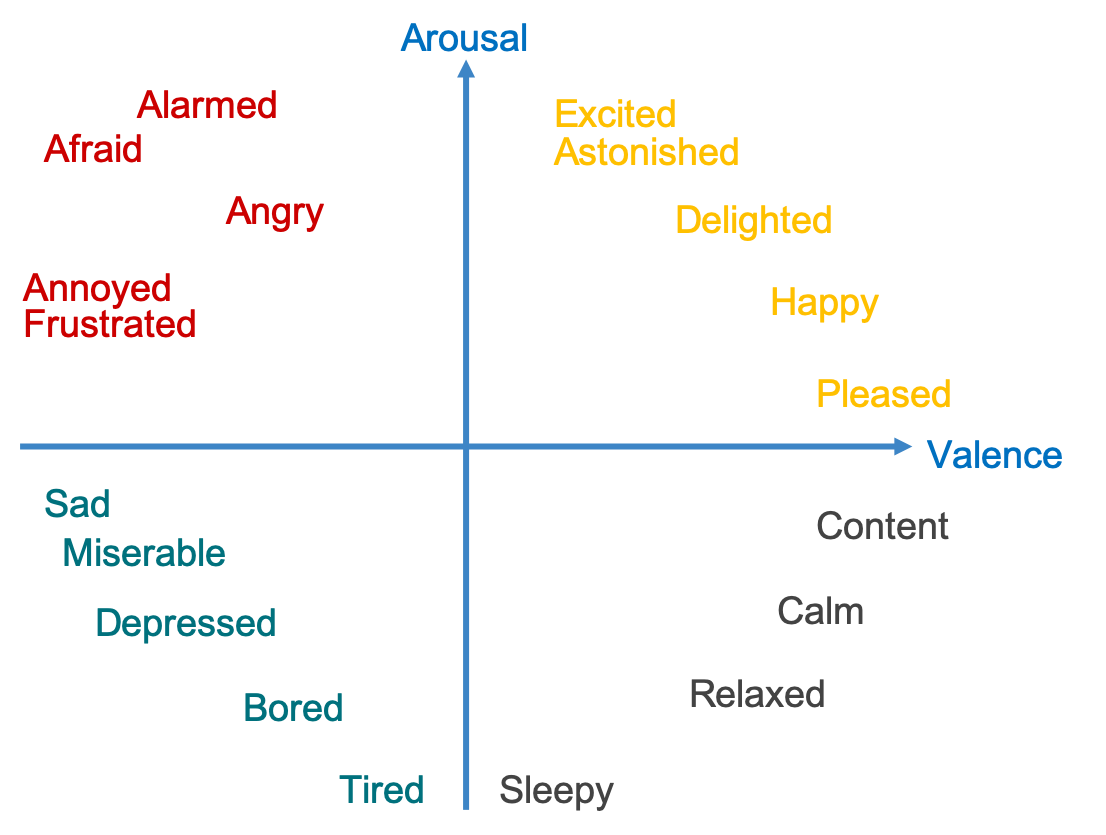
\includegraphics[width=10cm]{images/background/arousal_valence.png}
    \caption{Arousal-Valence dimension space with exemplar emotions}
    \label{fig:arousal_valence}
\end{figure}


Affective Computing is an interdisciplinary field that focuses on the study and development of systems that can recognize, interpret, process and express human affects. It spans Computer Science, Psychology, and Cognitive Science. Affect-sensitive interfaces are being developed in a number of domains to automatically recognizing and responding to users' affective states, including gaming, mental health, and learning technologies \cite{calvo2010}. For instance, an affect-sensitive tutoring system, called AutoTutor, could simulate human tutors and improve students' learning gains by detecting their emotional responses, like frustration \cite{sidney2005}.









\section{Mental Disorder Detection}

With the advancement in the field of Affective Computing, a large set of affective issues have been tackled, ranging from short-term states (e.g. laughter, emotions), to mid-term disorders (e.g. depression, bipolar disorder, or autism) and to long-term traits (e.g. personality traits) \cite{picard2000, schuller2011}. 

While the discrete emotions could be detected in shorter frames, the recognition of mid-term disorders needs to detect distinct emotions to indicate disorders as healthcare professionals do, and also take into account of temporal information \cite{picard2000, yacoob1994, zacharatos2014}. Temporal descriptors for both acoustic and visual modalities have been shown to provide more information for mental disorder detection \cite{ambadar2005, joshi2013}. Within the past several years, various models have been investigated for depression level estimation from behavioural observations \cite{cohn2007, cummins2011}, such as Gaussian Mixture Models (GMM), Support Vector Machines, Relevance Vector Regression (PVR), and even Deep Neural Networks (DNN). These proposed models proved promising results in some challenges, and for example, GMMs achieved an F1 mean score 0.81 in a binary depression detection compared with 0.73 in the baseline system \cite{williamson2016}. The automated approach for depression evaluation can be transferred to the detection of other mental disorders, such as bipolar disorder (BD).




\section{Audio-Visual Feature Extraction}

Arguably, the most important step in the automatic recognition of BD or other emotion-related tasks is the extraction of audio-visual features that must be relevant and provide a compact representation of each sample \cite{schuller2011}. The following subsections will discuss three commonly used audio-visual features in Affective Computing.



\subsection{MFCC}

In speech processing, Mel-Frequency Cepstrum Coefficients (MFCCs) have been the dominant features because of their ability to represent the speech amplitude spectrum in a compact form \cite{young1993htk}. Figure \ref{fig:mfcc_procedure} shows the procedure of the generation of MFCC features. The first step is to divide the audio signal into frames with equal length, usually by applying a window function, typically a Hamming window. The window function removes edge effects or noise in the background. A cepstral feature vector is then generated for each frame and Discrete Fourier Transform is applied on the vector. In the next step, only the logarithm of the amplitude spectrum is retained as amplitude is proven more important than phase information. Before taking a discrete cosine transform, the vector is Mel-scaled and smoothed first to emphasize perceptually meaningful frequencies. The Mel-scale relates perceived frequency, or pitch, of a pure tone to its measured frequency. The formula for converting from frequency to Mel scale is as follows.

\begin{equation}
    M(f) = 1125 \ln(1+f/700)
\end{equation}


\begin{figure}[htb]
    \centering
    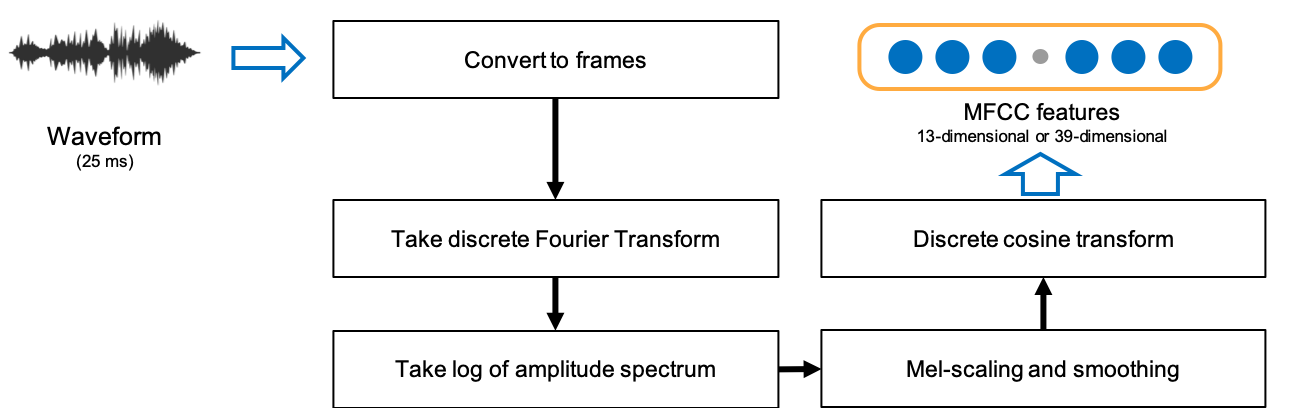
\includegraphics[width=12cm]{images/background/mfcc_procedure.png}
    \caption{MFCC features generation procedure}
    \label{fig:mfcc_procedure}
\end{figure}

The components in resulting Mel-spectral vectors for each frame are highly correlated and then Discrete Cosine Transform is used to decorrelate these components, generating 13 cepstral features on frame level. Generally, MFCCs from 25ms audio frames (sampled at a rate of 10ms) have dimensionality 13 from 26 Mel-Frequency bands. Additional 13 delta ($1^{st}$-order derivative) and 13 acceleration ($2^{nd}$-order derivative) coefficients could be appended to the MFCCs with a cepstral filter with a weight parameter of 22. MFCCs are commonly used as low-level descriptors (LLDs) in many audio signal processing tasks.




\subsection{GeMAPS and eGeMAPS}

Much of recent research considers the extraction of acoustic features as a method to understand the patterning of the vocal expression of different emotions \cite{juslin2001, yildirim2004, eyben2015}. The underlying theoretical assumption is that the affective processes influence autonomic arousal and the tension of the striated musculature at different scales and thus affect voice and speech production \cite{scherer1986}. These emotion-differentiating changes, if measured and extracted as a compact parameter set, could probably improve the performance recognition systems in BD.

Following this principle, Eyben \textit{et al.} proposed GeMAPS (and eGeMAPS) as a standard acoustic parameter set for voice analysis. GeMAPS stands for the Geneva Minimalistic Acoustic Parameter Set and it is a basic standard acoustic parameter set for various areas of automatic voice analysis. These parameters are selected based on the potential to index affective physiological changes in voice production, the proven value in former studies as well as the automatic extractability, and the theoretical significance. eGeMAPS, on the other hand, is the extended version of GeMAPS with additional cepstral parameters, and the full list refers to Table \ref{tab:list_egemaps}.

\begin{table}[ht]
    \small
    \centering
    \caption{Complete list of GeMAPS and eGeMAPS (parameters \textbf{in bold} are additional parameters only in eGeMAPS)}
    \begin{tabular}{p{3.5cm}|p{9cm}}
        \Xhline{2\arrayrulewidth}
        Parameter Name & Description \\
        \hline
        \multicolumn{2}{l}{Frequency Related Parameters} \\
        \hline
        Pitch & Logarithmic fundamental frequency $F_0$ on a semitone frequency scale \\
        Jitter & Deviations in individual consecutive $F_0$ period lengths \\
        Formant 1, 2, and 3 frequency & Centre frequency of 1st, 2nd, and 3rd formant \\
        Formant 1 & Bandwidth of 1st formant \\
        \textbf{Formant 2-3} & Bandwidth added for completeness \\
        \hline
        \multicolumn{2}{l}{Amplitude Related Parameters} \\
        \hline
        Shimmer & Difference of the peak amplitudes of consecutive $F_0$ periods \\
        Loudness & Estimate of perceived signal intensity from an auditory spectrum \\
        Harmonics-to-Noise Ratio & Relation of energy in harmonic components to energy in noise-like components \\
        \hline
        \multicolumn{2}{l}{Spectral Related Parameters} \\
        \hline
        Alpha Ratio & Ratio of the summed energy from 50-1000 Hz and 1-5 kHz \\
        Hammarberg Index & Ratio of the strongest energy peak in region 0-2kHz to the strongest peak in region 2-5 kHz \\
        Spectral Slop & Linear regression slope of the logarithmic power spectrum within 0-500 Hz and 500-1500 Hz \\
        Formant 1, 2, and 3 relative energy & Ratio of the energy of the spectral harmonic peak at 1st, 2nd, 3rd formant's centre frequency to the energy of the spectral peak at $F_0$ \\
        Harmonic difference H1-H2 & Ratio of energy of the first $F_0$ harmonic (H1) to the energy of the second $F_0$ harmonic (H2) \\
        Harmonic difference H1-A3 & Ratio of energy of the first $F_0$ (H1) to the energy of the highest harmonic in the third formant range (A3) \\
        \textbf{MFCC 1-4} & Mel-Frequency Cepstral Coefficients 1-4 \\
        \textbf{Spectral flux} & Difference of the spectra of two consecutive frames \\
        \Xhline{2\arrayrulewidth}
    \end{tabular}
    \label{tab:list_egemaps}
\end{table}





\subsection{Facial Action Units}

Facial behaviour can be defined as \textit{facial landmarks}, \textit{head pose}, \textit{eye gaze}, and \textit{facial expressions}, each of which plays an important role individually and collectively \cite{baltrusaitis2018}. Facial landmarks allow us to understand facial expression motion and the dynamics along with the benefits for face alignments in various tasks such as gender detection and age estimation \cite{fu2010age}. Head pose has been demonstrated its usefulness in emotion recognition and social signal perception \cite{adams2015}, and eye gaze has also been proved effective when evaluating attentiveness, social skills, mental health \cite{vail2017}, and intensity of emotions \cite{kleinke1986}. Facial expression, usually represented by Facial Action Units (FAUs), is both powerful and natural mean of inter-personal communication and emotions can be interpreted as a complex combination of several facial expressions \cite{ekman2013}. To detect and measure a large number of facial expressions, Ekman and Friesen \cite{ekman1976} developed the Facial Action Coding System (FACS), which is widely used for facial behaviour analysis to date. Their approach was, however, expensive and time-consuming as the selection of AUs was based on a small set of muscular actions observed and manually scored by the trained experts \cite{ekman1976}. Therefore, for automatic facial behaviour analysis and understanding, a system capable of recognizing \textit{facial landmarks}, \textit{head pose}, \textit{eye gaze}, and \textit{FAUs} without human intervention has been an active research topic.


\begin{figure}[ht]
    \centering
    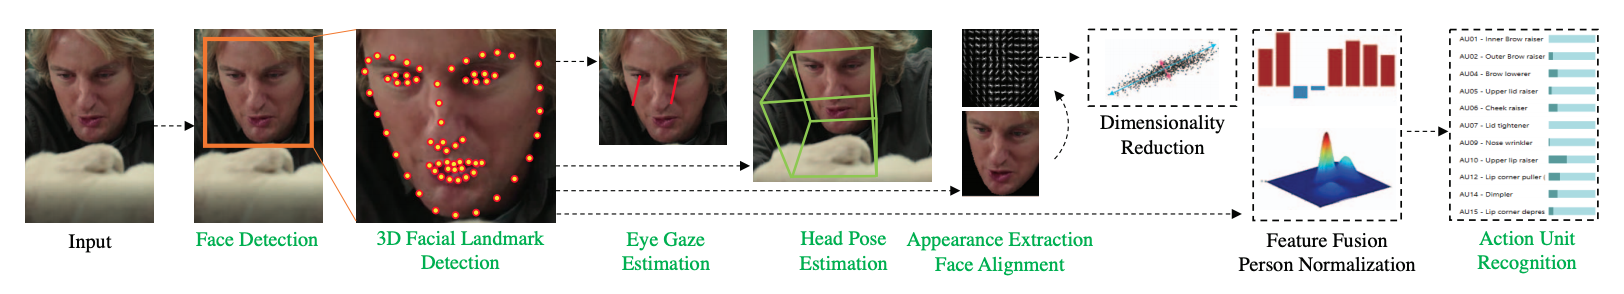
\includegraphics[width=1.1\textwidth]{images/background/openface.png}
    \caption[OpenFace 2.0 facial behaviour extraction pipeline]{OpenFace 2.0 facial behaviour extraction pipeline (taken from \cite{baltrusaitis2018})}
    \label{fig:openface}
\end{figure}


OpenFace 2.0, proposed by Baltrusaitis \textit{et al.} \cite{baltrusaitis2018} was an automatic toolkit on real-time data for facial landmark detection, head pose estimation, eye gaze determination, and facial action units recognition. The general pipeline of OpenFace 2.0 refers to Figure \ref{fig:openface}. OpenFace 2.0 was demonstrated state-of-the-art results in their experiment \cite{baltrusaitis2018}, and was used as the baseline extractor for visual features in many studies in Affective Computing communities. 



\section{Multimodal Learning}

Intuitively speaking, we interact with the surrounding world in different ways - we see objects, we hear sounds and we smell odours - and in other words, the world involves multiple modalities. A modality refers to a particular mode in which something happens or is experienced. When a research problem or dataset includes multiple modalities, it can be therefore characterized as multimodal. 


Multimodal learning is intended to build models that can process and relate information from multiple modalities \cite{baltruvsaitis2017}. Multimodal learning has been introduced with the motivation of the McGurk effect \cite{mcgurk1976} in Audio-Visual Speech Recognition (AVSR) that the visual input has been demonstrated influential in speech perception. In the following research, the experimental results showed that supplementary modalities, such as visual information in AVSR, improve the robustness of the multimodal models \cite{gurban2008} and the performance of the model in noisy scenarios \cite{ngiam2011}. 

In addition to AVSR, multimodal learning has also been applied to the automatic understanding of human multimodal behaviors in social interactions \cite{baltruvsaitis2017}. With the technical advances in face detection, facial landmark localization, and facial expression recognition \cite{kanade2005}, Audio-Visual Emotion Challenge (AVEC) has been introduced in 2011 to further the multimodal information processing and its application in healthcare and emotion recognition \cite{schuller2011}.

In my work, I only concentrate on three modalities, visual signals which are represented with images or video, acoustic signals which encode sounds and para-verbal information, and natural language which is spoken by the interview subjects. 

\chapter{Related Work}
\label{ch:literature}


In this chapter, a comprehensive overview of the Bipolar Disorder Corpus is firstly provided. The literature is then given on the automatic recognition systems of bipolar disorder and AVEC2018 challenge that builds the platform for these competing systems. Some depression detection systems using multimodal data are reviewed as they share many similarities as the BD recognition system.



\section{Bipolar Disorder Corpus}
\label{sec:bp-corpus}

Bipolar disorder (BD) is a major public health problem, with estimates of lifetime prevalence in the general population of the United States at 3.9 percent, with a range from 1.5 to 6.0 percent \cite{world2017, hilty2006}. BD patients tend to have higher probability of suicide, in which approximately 25 percent attempting it and 11 percent completing it \cite{prien1990}. For medical care in BD, two challenges remain, namely access to treatment and treatment resistance \cite{bauer2017}. In spite of the recent advance in the automatic recognition of human behaviours or depression severity, a dedicated BD corpus is required to find biological markers or predictors of treatment response and to reduce treatment resistance. 

The Turkish Audio-Visual Bipolar Disorder (BD) Corpus is a new dataset for the affective computing and psychiatric communities \cite{cciftcci2018}. The corpus is also expected to provide an insight for the personalized treatment of BD patients \cite{cciftcci2018}. The corpus is annotated for BD states as well as the Young Mania Rating Scale (YMRS) by psychiatrists following DSM-5's inclusion criteria \cite{american2013}. More specifically, the YMRS scores are obtained at session level such that each score corresponds to one patient on one of the test days: $0^{th}$ day, $3^{rd}$ day, $7^{th}$ day, $14^{th}$ day, $28^{th}$ day, $90^{th}$ day. The data format in the corpus is a set of audio-visual recordings of structured interviews performed by 46 Turkish speaking objects (49 healthy controls). During the interviews, participants were asked to complete seven tasks as shown in Table \ref{tab:question}, and the two emotion-eliciting pictures used are displayed as Figure \ref{fig:drawing}.

\begin{table}[ht]
    \centering
    \caption{List of questions in the structured interviews of BD corpus}
    \begin{tabular}{l|l|l}
        \Xhline{2\arrayrulewidth}
        index & required task & topic \\
        \hline
        1 & Describe why you come here & negative task \\
        2 & Depict Van Gogh's \textit{Depression} & negative task \\
        3 & Describe the worst memory & negative task \\
        \hline
        4 & Count 1 - 30 & neutral task \\
        5 & Count 1 - 30 again (usually faster) & neutral task \\
        \hline
        6 & Depict Dengel's \textit{Home Sweet Home} & positive task \\
        7 & Describe the best memory & positive task \\
        \Xhline{2\arrayrulewidth}
    \end{tabular}
    \label{tab:question}
\end{table}

\begin{figure}[ht]
    \centering
    \begin{minipage}[c]{0.30\textwidth}
    \centering
    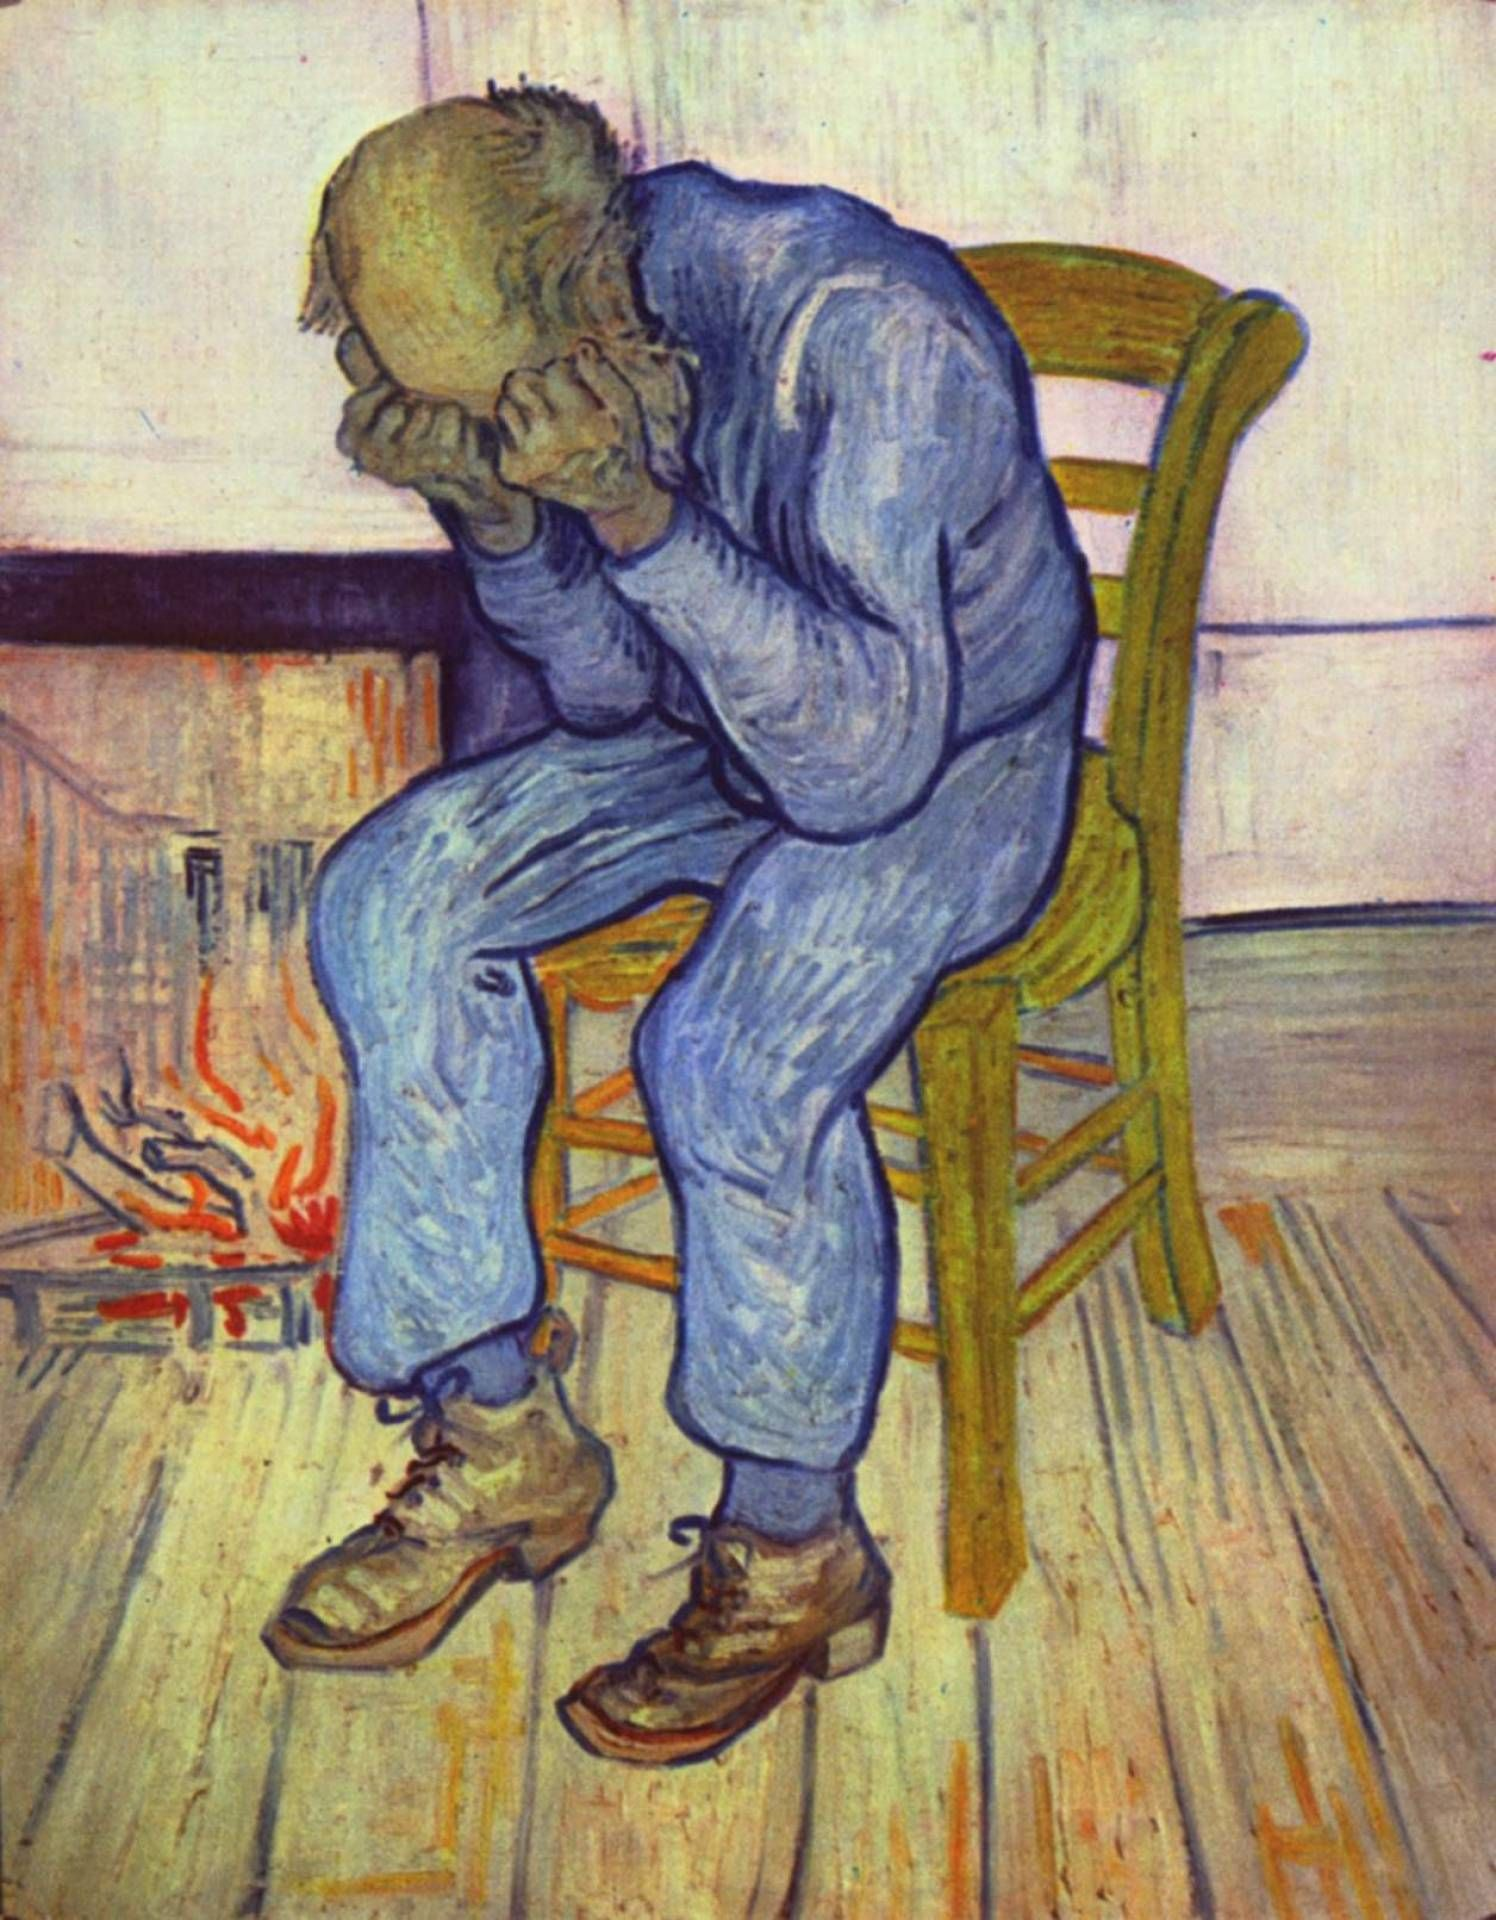
\includegraphics[height=5cm]{./images/dataset/dataset_depression.jpg} \\
    van Gogh's \textit{Depression}
    \end{minipage}
    \begin{minipage}[c]{0.55\textwidth}
    \centering
    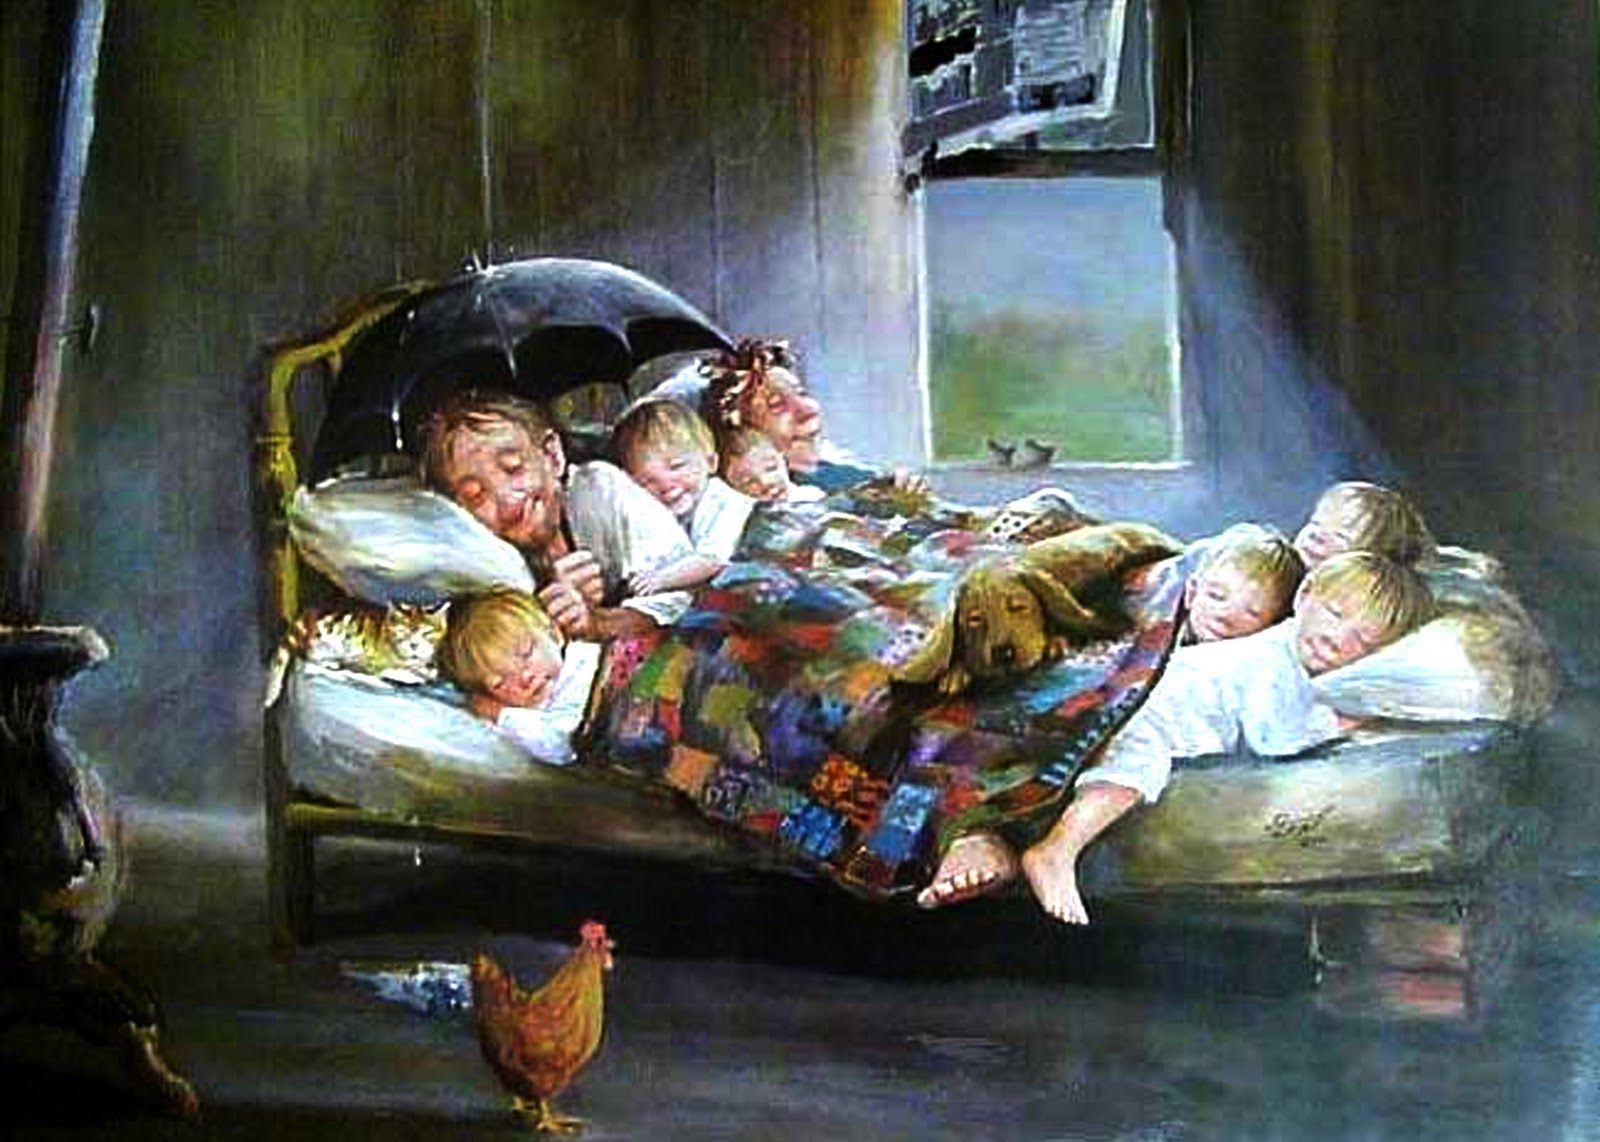
\includegraphics[height=5cm]{./images/dataset/dataset_sweet_home.jpg} \\
    Dengel's \textit{Home Sweet Home}
    \end{minipage}
    \caption{Two emotion eliciting pictures used in the structured interviews.}
    \label{fig:drawing}
\end{figure}

In the corpus, a total of 50 bipolar manic patients (34 male and 16 female) aged between 18 to 54 years are recorded along with 39 healthy controls (23 male and 16 female) aged between 18 to 57 years. Sociodemographics and clinical statistics for two groups are listed in Table \ref{tab:demographic}. 

\begin{table}[ht]
    \small
    \centering
    \caption{Demographic and clinical statistics of BD group and healthy control group}
    \small
    \begin{tabular}{p{1.8cm}|c|c|c|c|c|c}
         \Xhline{2\arrayrulewidth}
         & \multicolumn{3}{c|}{Patients with BD} & & & \\
         & Female & Male & All & Healthy & $t/x^2$ & $p$  \\
         \hline
         Age & $40.2\pm8.8$ & $35.02\pm10.6$ & $36.7\pm10.3$ & $37.3\pm10.9$ & 0.36 & 0.72 \\
         \hline
         Education & $12.6\pm2.9$ & $9.5\pm3.3$ & $10.5\pm3.5$ & $11.2\pm3.7$ & 0.89 & 0.11 \\
         \hline
         Total Episode & $7.13\pm7.7$ & $7.67\pm5.7$ & $6.26\pm6.4$ & - & 0.71 & 0.48 \\
         \hline
         Illness Duration & $15.9\pm9.9$ & $12.02\pm9.7$ & $13.07\pm9.8$ & - & 1.41 & 0.16 \\
         \Xhline{2\arrayrulewidth}
    \end{tabular}
    \label{tab:demographic}
\end{table}


For the classification experiments, the corpus contains 104 recordings as the training partition, 60 recordings as the development partition, and 54 recordings as the test partition, simultaneously balancing the gender distribution. The statistics of recordings refer to Table \ref{tab:recording_length}. The provided ground-truth labels are clinician-annotated YMRS scores of corresponding sessions, and the recordings are also grouped into three disjoint subgroups as follows, thus leading to a ternary classification task.

\begin{itemize}
    \item Remission / Depression: YMRS $\leq$ 7
    \item Hypo-mania: 7 $<$ YMRS $<$ 20
    \item Mania: YMRS $\geq$ 20
\end{itemize}


\section{AVEC2018 Challenge}

Since the automatic recognition of Bipolar Disorder (BD) is recently introduced along with a Turkish-speaking BD corpus, the literature is limited except for the work in the Audio/Visual Emotion Challenge and Workshop (AVEC 2018). AVEC 2018 presented three sub-challenges, and one was BD recognition with Turkish Audio-Visual BD corpus \cite{cciftcci2018}. The organizers \cite{ringeval2018} presented the baseline system for BD recognition, in which only low-level descriptors (LLDs), extracted with open-source toolkits, were used in linear SVM classifiers and the final decision was based on a late fusion of best-performing audio and video representations. In the audio modality, they investigated MFCCs, eGeMAPS, and DeepSpectrum features. DeepSpectrum features were firstly introduced for snore sound classification \cite{amiriparian2017}. Heavily inspired by image processing, DeepSpectrum features were extracted from Mel-spectrogram using the activations from the $2nd$ fully-connected layer of \textit{ALEXNET}. On the other hand, Facial Action Units (FAUs) were used as visual features in the baseline system. The unweighted average recall (UAR) of three symptoms of BD was set as scoring metric, and the best performance on the development partition in the baseline system was 0.635 UAR with the fusion of DeepSpectrum and FAUs.


\begin{table}[htb]
    \centering
    \caption{Comparison of four proposed BD recognition systems in AVEC 2018. The best results are in \textbf{bold} for each metric, and ``dev" and ``test" indicate the performance respectively measured in the development and test set.}
    \begin{tabular}{l|l|l}
        \Xhline{2\arrayrulewidth}
        system & UAR (dev / test) & Accuracy (dev / test) \\
        \hline
        Yang \textit{et al.} 2018 & 0.714 / \textbf{0.574} & \textbf{0.717} / NA \\
        \hline 
        Du \textit{et al.} 2018 & 0.651 / NA & 0.650 / NA \\
        \hline 
        Xing \textit{et al.} 2018 & \textbf{0.868} / \textbf{0.574} & NA / NA \\
        \hline
        Syed \textit{et al.} 2018 & 0.635 / \textbf{0.574} & NA / NA \\
        \Xhline{2\arrayrulewidth}
    \end{tabular}
    \label{tab:four_results}
\end{table}

Against the baseline system, four participating teams presented their BD recognition systems. Yang \textit{et al.} \cite{yang2018} proposed several effective features for the classification: histogram based arousal features, features about speaking rate, and histogram based hands distance features. Along with other histograms of LLDs, these features were reduced in dimensionality and then concatenated before feeding into tree-based classifiers. The histogram-based features enabled the following classification on session-level and the final decision was obtained through a majority vote on an ensemble learning strategy to overcome overfitting issues. The features in visual modality, however, might not capture rapid changes as only histograms emphasized the distribution instead of temporal dependency between features per frame. Moreover, without considering the correlation between modalities, the features lacked robustness as seen in the gap between the performance of development set and test set (shown in Table \ref{tab:four_results}). 

Du \textit{et al.} \cite{du2018} presented a new model called IncepLSTM to encode audio temporal representation on multiple scales with convolutional kernel sizes 1, 3, and 5 in Inception module \cite{szegedy2015}. With an improved triplet loss function to emphasize model sensitivity to the YMRS score, they claimed success to capture dynamic information and to obtain a high-level descriptor for the whole audio clip. Nevertheless, the performance on the development partition is relatively low as seen in Table \ref{tab:four_results} because they only took into account the acoustic modality, resulting in an incomplete utilisation of the available multi-modalities.

Xing \textit{et al.} \cite{xing2018} made full use of all modalities in their framework, including audio, video, and text, which was transcribed with Google Cloud Platform (GCP)\footnote{\url{https://cloud.google.com/translate/}}. They also introduced a hierarchical recall model for the classification, where patients with different mania level were recalled at multiple levels. Each layer within the model contained a Gradient Boosted Decision Tree (GDBTs) using different subsets of all features, and following a boosting strategy, the only un-recalled samples would be transmitted to the next layer. Although the proposed framework yields the highest UAR in the development partition of the four systems, it does not outperform others in the test partition, which indicates their framework might suffer from overfitting due to the noisy data or the limited corpus.

Syed \textit{et al.} \cite{syed2018} proposed ``turbulence features" to capture sudden, erratic changes in feature trajectories, which was measured as the crest factor, the ratio between the absolute maximum value of the signal and its root mean square value, within each window. They applied Fisher Vector (FV) encoding of one modality in feature aggregation and Greedy Ensembles of Weighted Extreme Learning Machines (GEWELMs) in classification. While ``turbulence features" might capture the irregularities in acoustic or visual features, the lack of multi-modal fusion at an early stage leads to the lowest UAR of the four systems as seen in Table \ref{tab:four_results}.




\section{Multimodal Depression Detection Systems}

In addition to the proposed frameworks in AVEC2018, previous research on speech recognition and emotion recognition has demonstrated the effectiveness of some deep architectures on multi-modal data. For audio-visual speech recognition, Ngiam \textit{et al.} \cite{ngiam2011} presented bimodal deep autoencoders to capture the correlations across different modalities and validated the deep architecture on CUAVE and AVLetters datasets. Since it would be difficult to correlate raw data of different modalities, both audio and visual modalities were fused in the shared hidden layer with the learnt first layer representations, which were called ``mid-level" representations \cite{ngiam2011}. Their approach inspired the following work on discovering multimodal features. For emotion recognition, Kim \textit{et al} \cite{kim2013} and Ranganathan \textit{et al.} \cite{ranganathan2016} proposed multi-modal Deep Belief Network (DBN) models, in which ``mid-level" representations on different modalities were connected to one shared hidden layer. With the bimodal representations, they showed an increase in classification performance when compared the baseline system on unimodal features.

Automatic recognition of BD or depression severity, on the other hand, differs from emotion recognition in the processing of temporal information \cite{picard2000, yacoob1994, zacharatos2014}. Dibeklio{\u{g}}lu \textit{et al.} \cite{dibekliouglu2017} presented Stacked Denoising Autoencoders (SDAE) to learn the non-linear mapping of facial landmarks and head pose on frame-level, which was determined by the feature extraction within a specific length of window. An improved Fisher Vector \cite{perronnin2010} was then applied to encode the per-frame representations of visual features into the per-video representations for measurement of depression severity. In their evaluation, dynamics facial landmarks outperformed other modalities and the majority voting \cite{kuncheva2002} of all three modalities showed higher accuracy than unimodal model. 


\chapter{Design and Implementation} 
\label{ch:design}




This chapter details the proposed framework and implementation. I start by giving an overview of the proposed framework, and then five crucial components in the framework are carefully explained: Deep Denoising Autoencoders on audio-visual modalities, Fisher Vector Encoding, Document Embedding on textual modality, Tree-based Feature Selection and Multi-Task Learning. 





\section{Overview}

Figure \ref{fig:pipeline} illustrates the framework of my proposed method for automatic Bipolar Disorder BD recognition. For acoustic modality, I extract 39-dimensional Mel-Frequency Cepstrum Coefficients (MFCCs)\footnotemark as the Low-Level Descriptors (LLDs) with OpenSMILE and for visual modality, I extract the 132-dimensional facial landmarks, 6-dimensional head pose, 6-dimensional eye gaze, and 35-dimensional Facial Action Units (FAUs) as the LLDs with OpenFace. To discover the correlation across audio-visual modalities and produce robust representations, I propose a Deep Denoising Autoencoder (DDAE) that learns a shared and joint representation on different number of modalities. More specifically, according to the number of modalities on which DDAEs are built, I define uni-DDAE, bi-DDAE, and multi-DDAE. Before feeding multimodal features into DDAE, features must be aligned on frame-level first to ensure they are extracted from the same time interval. I then compute the dynamic changes of the latent representations in DDAE as each representation is regarded as a specific movement of the subject. After computing the velocity ($1^{st}$-order derivative) and the acceleration ($2^{nd}$-order derivative) of the latent representations, the three features are concatenated as frame-level descriptors. Because the video clips vary in length, I encode the frame-level descriptors with a Fisher Vector (FV), a fixed-length descriptor on session-level, by fitting them into a Gaussian Mixture Model (GMM). To reduce redundancy and select the most discriminative feature set, a tree-based model is used for feature selection by evaluating the feature importance.


\begin{figure}[ht]
    \centering
    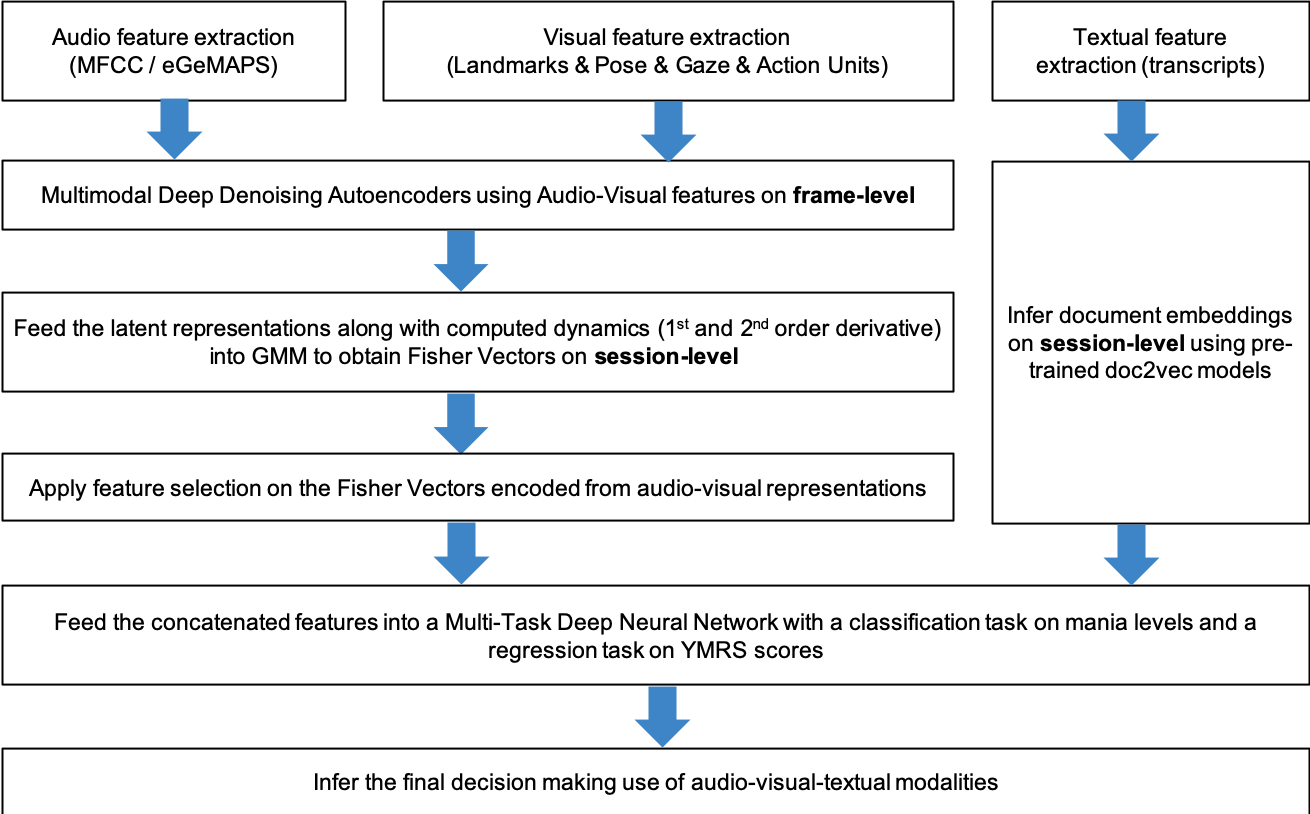
\includegraphics[width=13.5cm]{images/design/general_pipeline.png}
    \caption{Pipeline of the proposed framework that includes different learning architectures on different modalities}
    \label{fig:pipeline}
\end{figure}

On the other hand, I obtain the transcripts of video interviews and apply a document embedding model (doc2vec) to learn fixed-length representations of the transcripts on session-level. To boost the performance of the doc2vec model, the model is pre-trained on an additional Turkish corpus. 

With both fixed-length FVs on audio-visual modalities and fixed-length document embeddings on textual modality, a Multi-Task Deep Neural Network (MT-DNN) is built to handle the overfitting due to the limited size of the BD corpus. The MT-DNN is learned with a weighted loss from the ternary classification task of Mania Level and the regression task of Young Mania Rating Scale (YMRS). Furthermore, to address the imbalance between three classes, I duplicate the training instances of the minority class and apply Unweighted Average Recall (UAR) as my metric for evaluation. Finally, with the best-performing MT-DNN, the final decision on each video interview is inferred: depression, hypo-mania, or mania.


\footnotetext{The 39-dimensional MFCC features are obtained by appending additional 13 delta and 13 acceleration coefficients to the conventional 13-dimensional MFCC features.}









\section{Deep Denoising Autoencoders}
\label{sec:DDAE}

Autoencoders (AEs) are an unsupervised learning algorithm that learns a latent-space representation of given data with hidden layers constrained while reconstructing the data from the representation. The representations learnt from AEs generally have a lower dimensionality and have been proven effective as high-level features in the following classification tasks, which in many cases are competitive or even superior to the hand-engineered representations \cite{ng2011}. Autoencoders are composed of two parts: a) encoder, which compresses the input into a latent representation with the function $h=f(x)$, and b) decoder, which reconstructs the input from the latent representation with the function $r=g(h)$, as shown in Figure \ref{fig:unimodal_ae}. Therefore, autoencoders can be described by the function $g(f(x))=r$, and the reconstruction error $\parallel x-r \parallel ^ 2$ is minimized in the training processing. 

\begin{figure}[ht]
    \centering
    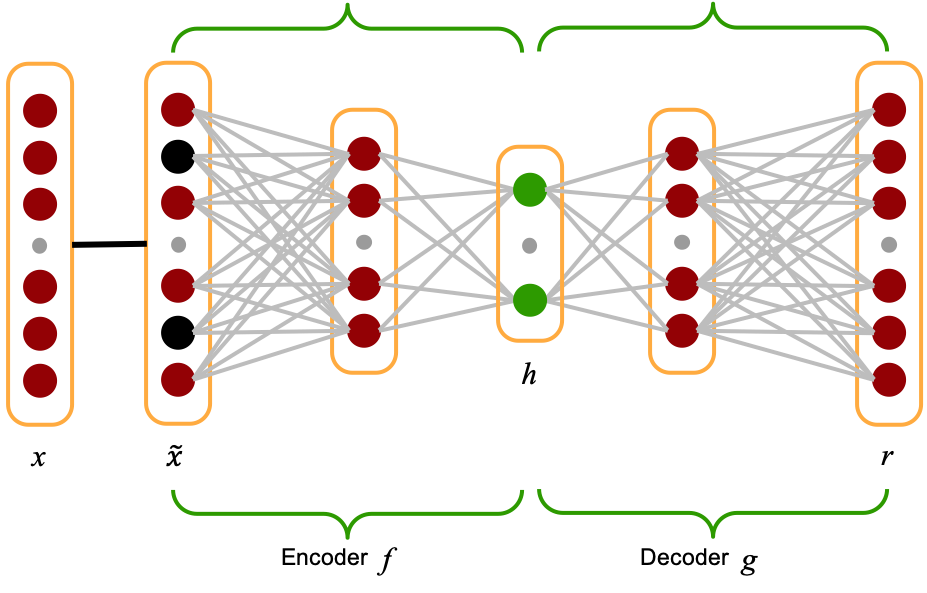
\includegraphics[height=6.5cm]{images/design/autoencoder.png}
    \caption{Schematic for Unimodal Deep Denoising Autoencoders}
    \label{fig:unimodal_ae}
\end{figure}


Autoencoders were first introduced as an approach to initialize the weights of neural networks \cite{ballard1987}, and because of the \textit{curse of dimensionality} \cite{bellman1966}, the low-dimensional hidden layers enable AEs to be commonly employed in feature engineering and representation learning \cite{charte2018}. Several variations of AEs have been developed with different constraints on the hidden layers, such as sparse AEs \cite{ng2011}, denoising AEs \cite{vincent2008}, and variational AEs \cite{kingma2013}. 

Denoising AEs, proposed by \cite{vincent2008}, stochastically corrupts part of the original input $x$ and reconstructs the original input $x$ with the corrupted version $\tilde{x}$. The noise can be of different forms, such as additive isotropic Gaussian noise and masking noise \cite{vincent2010}. The Gaussian noise $\tilde{x}$ is obtained with $\tilde{x}|x \sim \mathcal{x, \sigma^2,I}$ and the masking noise is calculated by forcing a fraction $v$ of the elements of input $x$ to 0. Although the Gaussian noise is reported to be the natural choice for real-valued inputs \cite{vincent2010}, I only consider the masking noise in the experiment as the Gaussian noise could introduce a small change in facial expressions, which could be interpreted as a misleading descriptor for the BD symptoms. The objective of denoising AEs accordingly becomes minimizing the reconstruction error $\parallel \tilde{x}-r \parallel ^ 2$. The denoising AEs are reported to produce representations that are robust to small irrelevant changes in the input.

With the development of multimedia data processing, a more recent learning architecture is introduced for feature fusion: the multi-modal AEs \cite{mangai2010}. Feature fusion aims to learn a shared representation cross modalities without redundant or irrelevant information, which is one of the biggest challenges in multi-modal data processing \cite{mangai2010}. In the work of \cite{hong2015}, authors aimed to perform multimodal fusion of 2D images and 3D human poses to obtain high-level representations. 
Inspired by \cite{vincent2008}, \cite{mangai2010}, and \cite{dibekliouglu2017}, I propose a series of 3-layer Deep Denoising Autoencoders (DDAEs) (i.e., DDAEs with 3 hidden layers) with different number of modalities to investigate the multimodal fusion in the BD detection task. 

\subsection{Unimodal Deep Denoising Autoencoders}

I first define the unimodal DDAEs on acoustic and visual features respectively as shown in Figure \ref{fig:unimodal_ae}, where features of one modality are fed into DDAEs to learn a compact-size representation after adding masking noise. This architecture is considered as a baseline for the following architectures as it does not discover the correlation across modalities. 

In many implementations of AEs, the binary cross-entropy (BCE) is set as the loss function, which measures the amount of information is preserved in the reconstruction compared to the original input \cite{de2005}. BCE is calculated with Equation \ref{eq:binarycrossentropy}, in which $x_k$ represents one node in the input layer and $r_k$ represents the corresponding node in the output layer. The input data must be therefore normalized to the range $[0,1]$ with the sigmoid activation function in the output layer. BCE could apply to binary-value image pixel intensities, such as MNIST dataset, because the range of original intensities lies in $[0, 255]$, but other features, like MFCC, rarely share the same range across the dataset and normalization could wrongly corrupt the correlation in features, thus hurting the extraction of emotion-related information. In my framework, instead, I define the loss function as the mean squared error (MSE) (Equation \ref{eq:mse}) with the linear activation function in the output layer and no normalization. The DDAEs are trained on minimizing the distance between reconstructed input and original input, and the reconstruction could be easily interpreted and visualized in the evaluation.

\begin{equation}
    J(x,r) = - \sum_{k=1}^d x_k \log(r_k) + (1-x_k) \log(1-r_k)
    \label{eq:binarycrossentropy}
\end{equation}

\begin{equation}
    J(x,r) = \frac{1}{N} \sum_{k=1}^d (x_k - r_k)^2
    \label{eq:mse}
\end{equation}


\begin{figure}[ht]
    \centering
    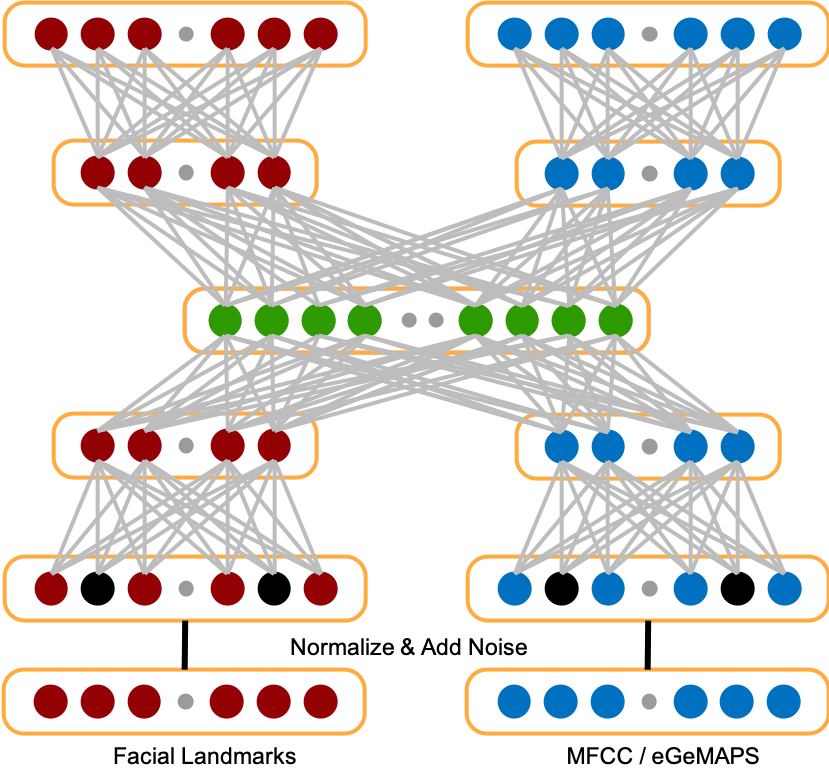
\includegraphics[height=7.5cm]{images/design/bimodal_ae.png}
    \caption{Schematic for Bimodal Deep Denoising Autoencoders (Different colours indicate different modalities)}
    \label{fig:bimodal_ae}
\end{figure}


\subsection{Bimodal Deep Denoising Autoencoders}

I continue to define the 3-layer bimodal DDAEs on acoustic and visual features altogether as displayed in Figure \ref{fig:bimodal_ae}. The acoustic features are Low-Level Descriptors (LLDs), either MFCC or eGeMAPS features, and the visual features in this architecture are set as facial landmarks whose dynamics have been proven useful in depression detection \cite{dibekliouglu2017}. As suggested in the work of \cite{ngiam2011}, two separate encoders are merged into one shared hidden layer after one hidden layer, which outputs the first-order representations. From the shared hidden layer, two modalities are then reconstructed via their decoders with the sum of MSE on both reconstructed inputs as the loss function. 
Acoustic and visual modalities need to be aligned beforehand to ensure they are within the same window \cite{ngiam2011}, and I concatenate 3 contiguous acoustic features as each input that has approximately the same duration as 1 visual feature. Because audio-visual modalities have different data formats and ranges, they are normalized and whitened separately.

\begin{figure}[ht]
    \centering
    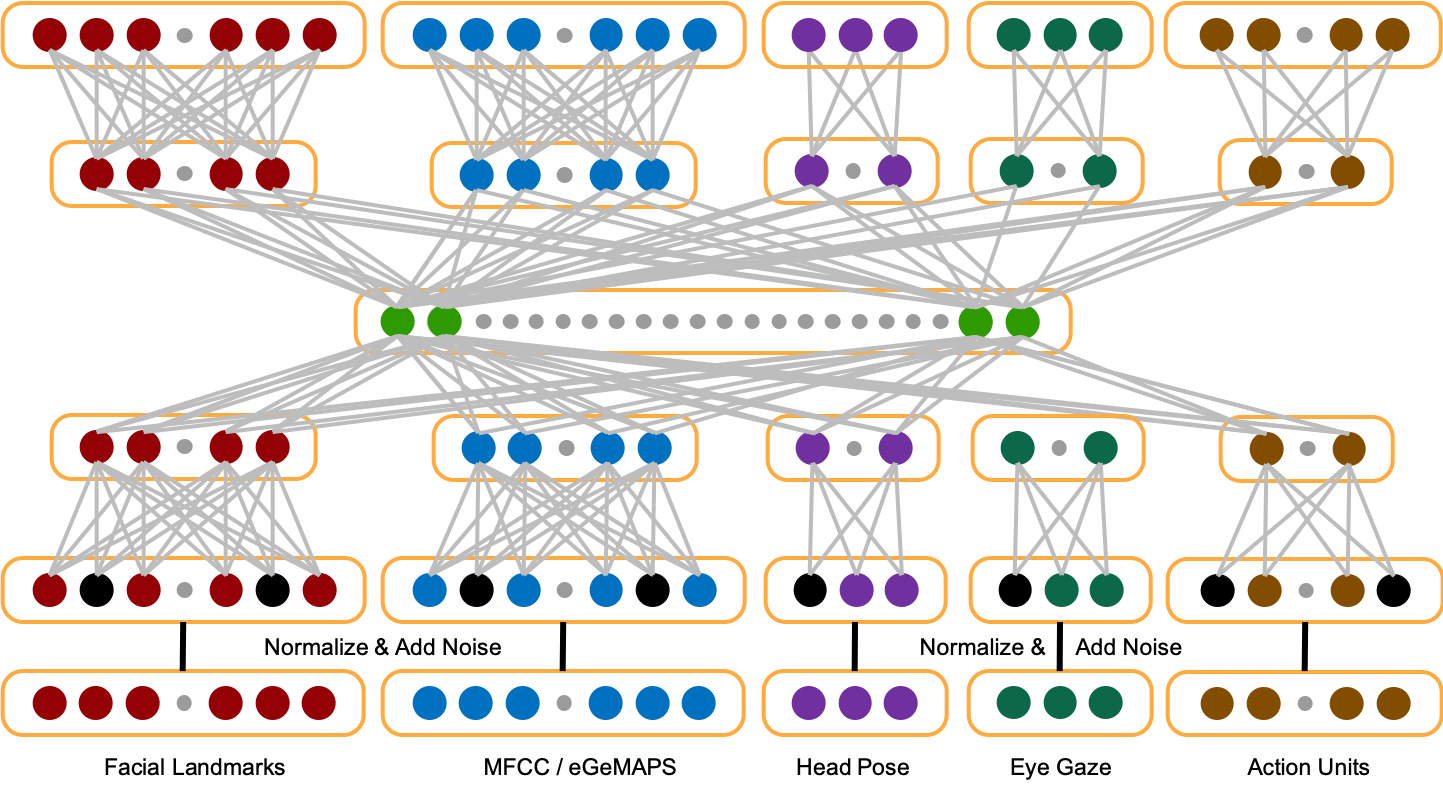
\includegraphics[height=7.5cm]{images/design/multimodal_ae.png}
    \caption{Schematic for Multimodal Deep Denoising Autoencoders (Different colours indicate different modalities)}
    \label{fig:multimodal_ae}
\end{figure}

\subsection{Multimodal Deep Denoising Autoencoders}

Given the importance of head pose, eye gaze, and action units in emotion recognition \cite{adams2015, ekman2013}, the 3-layer multimodal DDAEs are defined on a total of five modalities, namely facial landmarks, MFCC / eGeMAPS, head pose, eye gaze, and action units (shown in Figure \ref{fig:multimodal_ae}). Following the same design principle as the bimodal DDAEs, five modalities are merged into the shared representation layer with their ``mid-level" representation output by their first hidden layer, and masking noise is added to modalities individually. The reconstruction loss of each modalities is assigned with equal weights in the joint reconstruction loss function. 

\subsection{Implementation Details}

The list of investigated hyperparameters for all DDAEs is given in Table \ref{tab:param_DDAE}, in which the hidden ratio is defined as the ratio between two consecutive hidden layers, and for instance, with hidden ratio 0.5, the dimensions of all hidden layers would be $\{0.5d, 0.25d, 0.5d\}$ where $d$ represents the input dimensionality. In addition, I evaluate the denoising effect in DDAEs by setting different masking noise levels.


\begin{table}[ht]
    \centering
    \caption{Hyperparameter settings to investigate for DDAEs}
    \begin{tabular}{l|l}
        \Xhline{2\arrayrulewidth}
        Hyperparameter & Values \\
        \hline
        hidden ratio & \{0.4, 0.5\} \\
        noise level & \{0.1, 0.2, 0.4\} \\
        batch size & 1024 \\
        learning rate & 0.01 \\
        epochs & 100 \\
        \Xhline{2\arrayrulewidth}
    \end{tabular}
    \label{tab:param_DDAE}
\end{table}

The dimensions of all input modalities are listed in Table \ref{tab:dim_modality}. Because the shared representation is trained from only one acoustic features, either MFCC features or eGeMAPS features are input into bimodal DDAEs (Table \ref{fig:bimodal_ae}) and multimodal DDAEs (Table \ref{fig:multimodal_ae}). The sum of the input dimensions would thus be either 300 or 252, and the shared representation has four different dimensions with different hidden ratio settings (either 0.4 or 0.5), as shown in the last two row of Table \ref{tab:dim_modality}. The dimension of facial landmarks is obtained by $x$ and $y$ coordinates of 68 landmarks, while to acoustic features, dimensions of MFCC and eGeMAPS are multiplied with 3 because of the alignment of audio-visual modalities.

The training of DDAEs can be considered as the unsupervised feature learning, in which more data benefit the encoding of DDAEs \cite{ngiam2011}. All DDAEs are therefore trained with all available labelled (training set and development set) and unlabelled (test set) audio-visual data. 

\begin{table}[ht]
    \centering
    \caption{Dimension of all five modalities. The two dimensions of representations in the last two rows are based on the different hidden ratios, defined in \ref{tab:param_DDAE}}
    \begin{tabular}{l|l}
        \Xhline{2\arrayrulewidth}
        Modality & Dimension \\
        \hline
        Facial Landmarks & 136 ($68 \times 2$) \\
        MFCC features & 117 ($39 \times 3$) \\
        eGeMAPS features & 69 ($23 \times 3$) \\
        Head Pose & 6 \\
        Eye Gaze & 6 \\
        Action Units & 35 \\
        \hline
        Sum of input (MFCC) & 300 \\
        Sum of input (eGeMAPS) & 252 \\
        \hline
        Representation (MFCC) & 48 (0.4) / 75 (0.5) \\
        Representation (eGeMAPS) & 40 (0.4) / 63 (0.5) \\
        \Xhline{2\arrayrulewidth}
    \end{tabular}
    \label{tab:dim_modality}
\end{table}

\subsection{Computing Dynamics of Latent Representations}

After training, each DDAE (unimodal, bimodal, or multimodal) learns a presentation for the per-frame extracted features. These representations, however, only encode the static element of the input, such as locations of facial landmarks or loudness of audio signal, but without any temporary information. Following the ideas proposed in \cite{dibekliouglu2017}, I extend these representations with the dynamics. Considering DDAE-based representations as a matrix $H \in \mathcal{R}^{n \times d}$, in which $n$ denotes the number of frames and $d$ the final dimension of representations. Each column in $H_i(i \in \{1,2...d\})$ corresponds to one node in the representation layer, or for example, to one static point in unimodal DDAEs. I then compute the first-order dynamics, velocity $V$, of $H$ by the $1^{st}$ derivative $V_i = \frac{d H_i}{dt}$, measuring the velocity of the change between per-frame representations. I continue to calculate the second-order dynamics, acceleration $A$, of $H$ by the $2^{nd}$ derivative $A_i = \frac{d^2 H_i}{d^2 t}$, measuring the acceleration of the change. To align $H$, $V$, and $A$, I discard the first two frames in each video sessions, and I concatenate $H$, $V$, and $A$ for the final representations on frame-level.






\section{Fisher Vector Encoding}
\label{sec:fisher}

Feature aggregation is an approach via which low-level descriptors (LLDs) can be summarised to produce fixed-length high-level descriptors on variable-length audio-visual recordings, which encodes more global information. Many approaches within feature aggregation exist, such as the Bag-of-Words (BoW) \cite{csurka2004} and the Fisher Vector (FV) \cite{perronnin2010}. In my framework, to encode the frame-level representations learnt from DDAEs into a fixed-length vector on session-level, I investigate and implement the improved Fisher Vector (FV) \cite{perronnin2010, sanchez2013}. The BoW representations are briefly explained first as they are one of the baseline features used in Chapter \ref{ch:evaluation}.

\subsection{Bag-of-Words Representation}

Bag-of-Words originates from natural language processing and as a semi-supervised representation learning, it represents the distribution of LLDs based on a dictionary or codebook learned from them \cite{csurka2004, peng2016}. Generally, BoW is composed of five steps: a) feature extraction, b) feature-preprocessing, c) codebook generation, d) feature encoding, and e) pooling and normalization. According to the modality of representations, BoW can be categorised into Bag-of-Audio-Words (BoAW) and Bag-of-Visual-Words (BoVW). The feature extraction is completed as described in Chapter \ref{ch:background} and these extracted LLDs are usually high dimensional and strong correlated. Principal Component Analysis (PCA), a statistical procedure, is therefore used in BoW to preprocess the LLDs to low-dimensional and de-correlated features \cite{peng2016}. For codebook generation, two approaches are often considered, (i) partitioning the feature space into regions, each represented by its centre, such as $k$-means \cite{bishop2006}, and (ii) using a generative model to capture the probability distribution of features, such as Gaussian Mixture Model (GMM) \cite{bishop2006}. With parameters indicating either cluster centres or parameters for GMM, the LLDs extracted from one video are encoded into a fixed-length vector via voting-based or reconstruction-based encoding method \cite{peng2016}. In the last step, a pooling operation is used to obtain a global per-video representation and normalization enables the representations to be invariant to the variable number of LLDs extracted from different videos \cite{peng2016}.

\subsection{Fisher Vector}

Fisher Vector (FV) extends the bag-of-words (BoW) representations to learn the distribution of LLDs with their mean and variance, and it is commonly used as a global image descriptors in image classification \cite{perronnin2010, krapac2011}. More recently, FV has become popular for a variety of applications in social signal processing, such as depression estimation \cite{jain2014, dhall2015} and emotion recognition \cite{kaya2015}, because it combines advantages of both the generative and discriminative approaches \cite{sanchez2013} in machine learning. In the workflow of FV encoding, a generative model, typically Gaussian Mixture Model (GMM), is firstly built on LLDs and the Fisher kernel is then computed from this generative model. FVs are quantified using first and second order statistics of the gradient of the sample log-likelihood with respect to GMMs' parameters \cite{sanchez2013}.

Formally, let $X = \{x_t; t=1...T\}$ be an element in the time-series representations with the number of frames, $T$. Let $\Theta = \{\mu_k, \Sigma_k, \pi_k; k=1...K\}$ be the parameter of a Gaussian Mixture Model (GMM) fitting the distribution of the representations where $\mu_i$ and $\Sigma_i$ are respectively the mixture mean vector and covariance matrix and priors of GMM. GMM estimates a probability distribution of multiple multivariate Gaussian distributions and it is trained while maximizing the likelihood $p(X|\Theta)$:

\begin{equation}
    \Theta^{*} = \arg \max_{\Theta} p(X|\Theta) = \arg \max_{\Theta} \prod_{i=1}^{N} p(x_i|\Theta)
\end{equation}

GMM associates each vector $x_t$ to a mode $k$ in the mixture with a strength given by the posterior probability:

\begin{equation}
    q_{tk} = \frac{\exp [-1/2 (x_t-\mu_k)^{T} \Sigma_k^{-1}(x_t-\mu_k)]}{\sum_{i=1}^{K} \exp [-1/2 (x_t-\mu_i)^{T} \Sigma_k^{-1}(x_t-\mu_i)]}
\end{equation}

For each mode $k$, the mean and covariance deviation vectors are defined as 

\begin{align}
    u_{jk} &= \frac{1}{N\sqrt{\pi_k}} \sum_{t=1}^T q_{tk}\frac{x_{jt}-\mu_{jk}}{\sigma_{jk}} \\
    v_{jk} &= \frac{1}{N\sqrt{2\pi_k}} \sum_{t=1}^T q_{tk}[(\frac{x_{jt}-\mu_{jk}}{\sigma_{jk}})^2 - 1]
\end{align}

where $j=1,2...D$ spans the vector dimensions. The FV of the time-series representations is the stacking of the vector $u_k$ and $v_k$ for each of the K modes in the Gaussian mixtures:

\begin{equation}
    \Phi(X) = [...u_k...v_k...]^T
\end{equation}

\subsection{Improved Fisher Vectors}

In addition to the traditional FV, the improved FV was introduced by \cite{perronnin2010} for better classification performance with the following ideas :
\begin{itemize}
    \item Power normalization. As the number of Gaussians increases, FV becomes sparser and the distribution of features becomes more ``peaky" around zero. The kernel is therefore replaced with the Laplacian kernel, which is more robust on sparse vectors, by applying the function $|z| \sign z$ to each dimension of the vector $\Phi(X)$. 
    \item $l_2$ normalization. Before using the representations in a linear model, the vector $\Phi(X)$ is further by the $l_2$ normalization to discard the video-independent information, or descriptors which are likely to occur in any video. FV thus focus on video-specific features.
\end{itemize}

I compute the Fisher Vectors using GMMs with empirically 16 or 32 Gaussian distributions \cite{syed2018, dibekliouglu2017} to estimate the distribution on DDAE-based $d$-dimensional representations. The resulting feature vectors are $96 \times d_{latent}$ dimensional ($16 \times 2 \times 3 \times d_{latent}$) or $192 \times d_{latent}$ dimensional ($32 \times 2 \times 3 \times d_{latent}$), where $d_{latent}$ denotes the dimension of latent representation learnt from DDAEs.





\section{Tree-based Feature Selection}

Feature selection is a key step to reduce redundancy and improve the accuracy of classifiers by selecting the most informative features \cite{hira2015}. The reduced dimensional features should preserve as much information as the original high-dimensional features do. Considering the high dimension of the obtained Fisher Vectors with respect to the limited size of the dataset, feature selection is deemed necessary in my framework. Many approaches have been proposed to select the discriminative features, such as Min-Redundancy Max-Relevance (mRMR) algorithm \cite{peng2005}, Analysis of Variance (ANOVA) \cite{moran1918}, and correlation-based feature selection (CFS) \cite{pudil1994}, I apply tree-based feature selection in my framework by evaluating and ranking the importance of each feature. More specifically, a Random Forest (RF) classifier is used to compute the information gain $(S,A)$ for a feature $A$ relative to a dataset $S$: 

\begin{equation}
    Gain(S,A) = Entropy(S) - \sum_{v \in values(A)} \frac{|S_v|}{|S|} Entropy(S_v)
\end{equation}

where $values(A)$ is the set of all possible values for feature $A$, and $S_v$ is the subset of $S$ for which feature $A$ has value $v$. As RF is robust to redundant features and insensitive to the irrelevant information, the resulting feature importance leads to a reliable and discriminative subset of features. The split criterion is preset as entropy, and the number of trees as 800, determined by the baseline system describe in Chapter \ref{ch:evaluation}. I select the top 100 features in the Fisher Vector ranked with the importance, and in other words, the dimension for features in audio-visual modality is 100.



\section{Document Embedding}

Since strong correlations have been found between interview contents and depression symptoms \cite{morales2016, pampouchidou2016}, analyzing emotion-related textual modality has been emerged as a new approach in depression detection. More specifically, the use of negatively-valenced words and pronouns has been stressed in \cite{morales2016}. To incorporate textural modality into my framework, I first transcribe the recordings from BD corpus into plain texts using Google Speech-To-Text API \footnote{\url{https://cloud.google.com/speech-to-text/}}, and then make use of Paragraph Vector (PV) \cite{mikolov2014} to embed to session-level transcripts into textual features of the same size.

The PV model, or doc2vec, is an unsupervised learning algorithm to learn the distributed representations of a variable-length piece of texts \cite{mikolov2014}, and it is usually considered as an extension of word2vec, which aims to learn the word representations \cite{mikolov2013}.  

\subsection{word2vec}

The two architectures within word2vec, Continuous Bag-Of-Words (CBOW) and Skip-Gram (SG), are variants of neural networks with one hidden layer \cite{mikolov2013}. While CBOW architecture takes the context words (multiple word vectors) as input and predicts the target word (one word vector), SG architecture infers the context words given the target word, as shown in Figure \ref{fig:word2vec}. 

Formally, in word2vec-CBOW architecture, the objective is to maximize the log probability of the target word given context words with Equation \ref{eq:cbow}.

\begin{equation}
    \frac{1}{T} \sum_{t=c}^{T-c} \log p(w_t | w_{t-c} ... w_{t+c})
    \label{eq:cbow}
\end{equation}

where $c$ indicates the size of context windows (which equals to 2 in Figure \ref{fig:word2vec}) and $T$ represents the length of the word sequence. On the other hand, in word2vec-SG architecture, the optimization function is based on the averaged log probability as Equation \ref{eq:sg}, where $c$ and $T$ share the same notations as Equation \ref{eq:cbow}.

\begin{equation}
    \frac{1}{T} \sum_{t=i}^{T} \sum_{-c\leq j \leq c} \log p(w_{t+j}|w_t)
    \label{eq:sg}
\end{equation}

A large $c$ means a broader context window and thus a higher probability to capture the semantics of the words, but it could also lead to more expensive computation \cite{mikolov2013}. Furthermore, since the high dimensionality of input vectors can easily cause difficulties in the computation of condition probability $p(w_O|w_I)$ obtained by the softmax function, shown in Equation \ref{eq:softmax}, where $w_O$ is denoted as the ``output vector", $w_I$ as the ``input vector", and $W$ as the weight matrix that is updated via backpropagation with loss function $E = -\log p(w_O|w_I)$. Mikolov \textit{et al.} \cite{mikolov2013efficient} proposed three optimization techniques to improve the quality of output vectors and also the training speed: hierarchical softmax, negative sampling, and subsampling \cite{mikolov2013, mikolov2013efficient}. 

\begin{equation}
    p(w_O|w_I) = \frac{\exp({v^{'}_{w_O}}^{T} v_{w_I})}{\sum_{w=1}^{W} \exp({v^{'}_w}^{T} v_{w_{I}})}
    \label{eq:softmax}
\end{equation}

As an efficient approach of computer softmax, the hierarchical softmax applies a binary tree to represent $W$ words in the output layer \cite{mikolov2013}, and the evaluation of $W$ nodes in the output weight matrix is therefore reduced to $\log_2 W$ nodes. An alternative to the hierarchical softmax is negative sampling: instead of updating the entire weight matrix, only a limited number of ``negative words" are selected to update the weights \cite{mikolov2013efficient}. The ideas underlying subsampling is straightforward: the most frequent words in a large corpus generally provides less semantic information, such as ``a", ``the" or ``some" \cite{mikolov2013efficient}. Subsampling of such words can decrease the number of training samples and also help the neural networks to assign higher weights to rare words, which reflects more emotion-related information.

\begin{figure}[ht]
    \centering
    \begin{minipage}{0.47\textwidth}
        \centering
        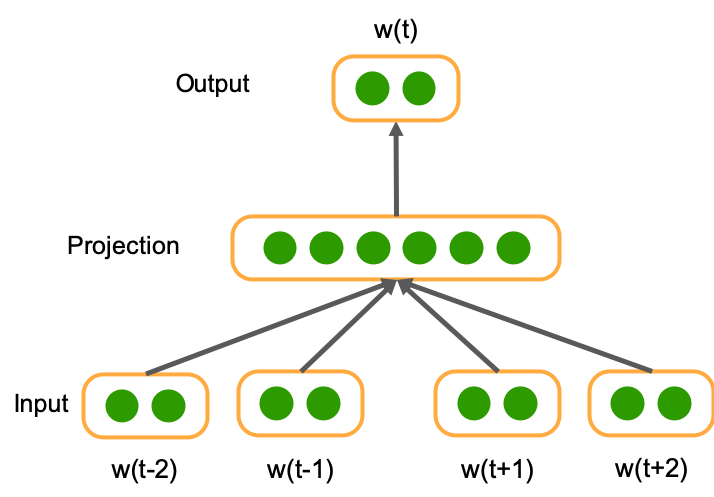
\includegraphics[height=4.3cm]{images/design/word2vec_cbow.png} \\
        (a) word2vec-CBOW
    \end{minipage}
    \begin{minipage}{0.48\textwidth}
        \centering
        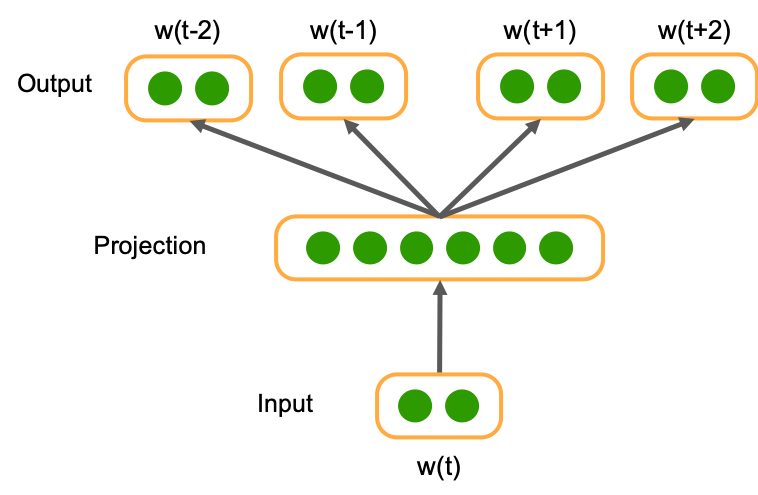
\includegraphics[height=4.3cm]{images/design/word2vec_sg.png} \\
        (b) word2vec-SG
    \end{minipage}
    \caption{Schematic for two Word Vector (word2vec) architectures}
    \label{fig:word2vec}
\end{figure}

\subsection{doc2vec}

To extend the embeddings to a higher level, the Paragraph Vector (doc2vec) is proposed to learn the representation for a variable-length of texts: sentence, paragraph and document. There are also two architectures within doc2vec, Paragraph Vector with Distributed Memory (PV-DM), corresponding to word2vec-CBOW, and Paragraph Vector with Distributed Bag-Of-Words (PV-DBOW), corresponding to word2vec-SG. As displayed in Figure \ref{fig:doc2vec}, both architectures introduce an additional document token that could be considered as the topic of each document (or in my framework, the mania level of transcript). The input in PV-DM is the concatenation of document vectors and word vectors, both of which are learned in the training process, but only the document vector is used for the inferring process. On the contrary, the PV-DBOW ignores the context words and predicts the words randomly sampled from the inferred document. It is obvious that PV-DBOW requires fewer data storage as it only saves softmax weights and PV-DM also needs to save the word vectors \cite{mikolov2014}. 

\begin{figure}[ht]
    \centering
    \begin{minipage}{0.55\textwidth}
        \centering
        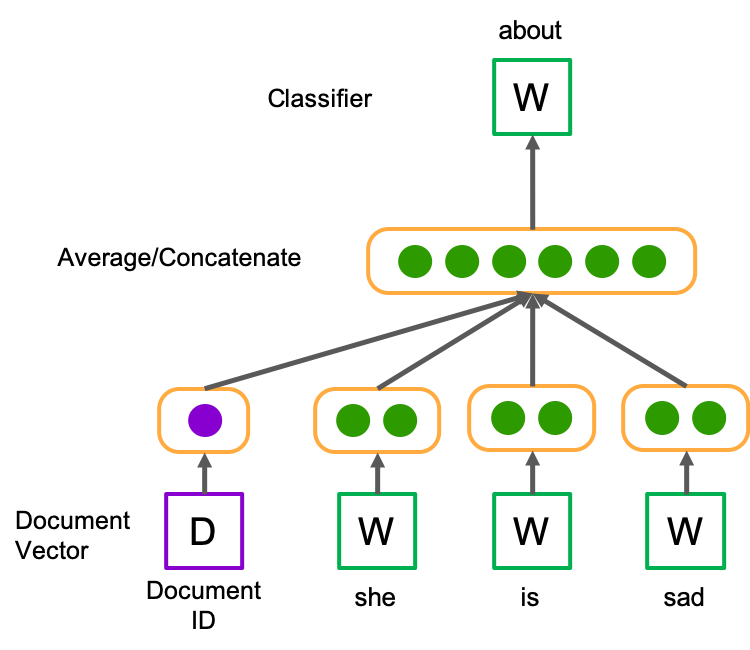
\includegraphics[height=5.4cm]{images/design/doc2vec_dm-m.png} \\
        (a) doc2vec-DM
    \end{minipage}
    \begin{minipage}{0.43\textwidth}
        \centering
        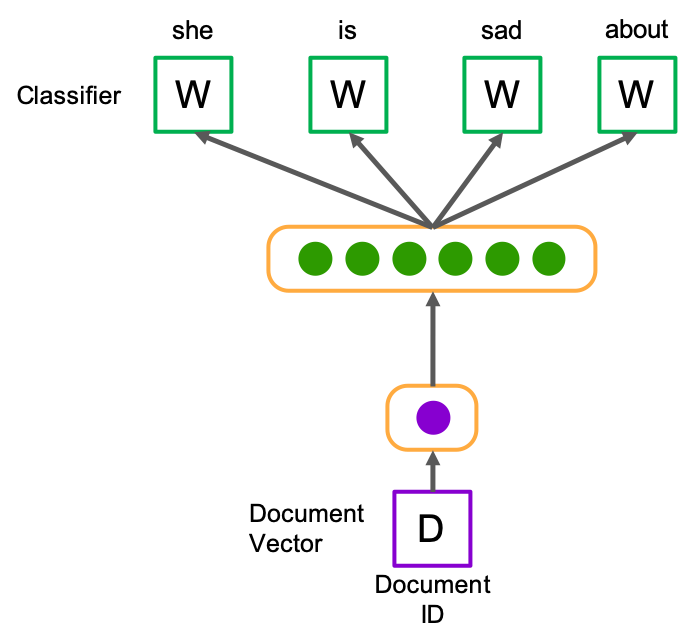
\includegraphics[height=5.4cm]{images/design/doc2vec_dbow.png} \\
        (b) doc2vec-DBOW
    \end{minipage}
    \caption{Schematic for two Paragraph Vector (doc2vec) architectures}
    \label{fig:doc2vec}
\end{figure}


\subsection{Implementation Details}
Some researchers have reported that PV-DBOW outperforms PV-DM in the sentiment analysis, contradictory results in the work of \cite{mikolov2014}. In addition, Yang \textit{et al.} only considers PV-DM architectures in their depression detection framework, and therefore, in my experiment, I investigate both PV-DM and PV-DBOW in the BD detection with different hyperparameter settings, as shown in Table \ref{tab:param_doc2vec}.


\begin{table}[ht]
    \centering
    \caption{Hyperparameter settings to investigate for document embedding}
    \begin{tabular}{l|l}
        \Xhline{2\arrayrulewidth}
        Hyperparameter & Values \\
        \hline
        model & \{PV-DM, PV-DBOW\} \\
        vector size & \{25, 50, 100\} \\
        window size & \{5, 10\} \\
        negative words & \{5, 10\} \\
        hierarchical softmax & \{0, 1\} \\
        \Xhline{2\arrayrulewidth}
    \end{tabular}
    \label{tab:param_doc2vec}
\end{table}

The translation of transcripts to English prior to the document embedding has been considered as it might help to understand the transcripts and to evaluate the embeddings. Nonetheless, I apply the doc2vec model directly on the Turkish transcripts to ensure the completeness of semantic content, which could be compromised in the translation, and after learning process, the document embeddings are evaluated with translation for better understanding. 

Due to the limited size of the BD corpus, I pre-train the doc2vec models on an external, large-scale Turkish corpus,``trwiki", to improve the performance of my models \cite{lau2016}. The ``trwiki" corpus is based on Wikimedia\footnote{\url{https://dumps.wikimedia.org/trwiki/}} dump service, which contains various kinds of texts in Turkish, such as articles, templates, media/file descriptions, and primary meta-pages. After training separate doc2vec models following the hyperparameter settings in Table \ref{tab:param_doc2vec}, I first evaluate their performance with a simple Random Forest (RF) classifier, the same classifier used in the baseline, and select the best-performing doc2vec model to infer the document vector for each transcript. These document vectors are used in the final fusion stage to predict the mania level of each session. In addition, visualizing the similar groupings of transcripts via Embedding Projector\footnote{\url{http://projector.tensorflow.org}} and the similar words stored in PV-DM models are presented to qualitatively examine the embedding space inferred by the doc2vec models.






\section{Multi-Task Learning}

In the context of Deep Learning, the generalization of the model could be improved if representations being shared across related tasks \cite{ruder2017}, and this approach is called Multi-Task Learning (MTL). There are two typical structures in MTL, hard parameter sharing and soft parameter sharing. Hard parameter sharing is applied by sharing the hidden layers between all tasks, with unchanged task-specific output layers (as shown in Figure \ref{fig:mtl}). Soft parameter sharing, on the other hand, separate all tasks with their own model and parameters (as shown in Figure \ref{fig:mtl}) with an objective to minimize the distance between parameters of different models.

\begin{figure}[ht]
    \centering
    \begin{minipage}[c]{0.42\textwidth}
    \centering
    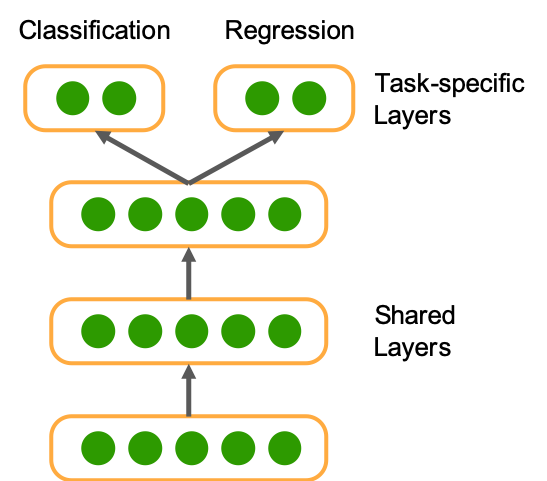
\includegraphics[height=4.2cm]{images/design/multitask_hard.png} \\
    (a) Hard parameter sharing
    \end{minipage}
    \begin{minipage}[c]{0.55\textwidth}
    \centering
    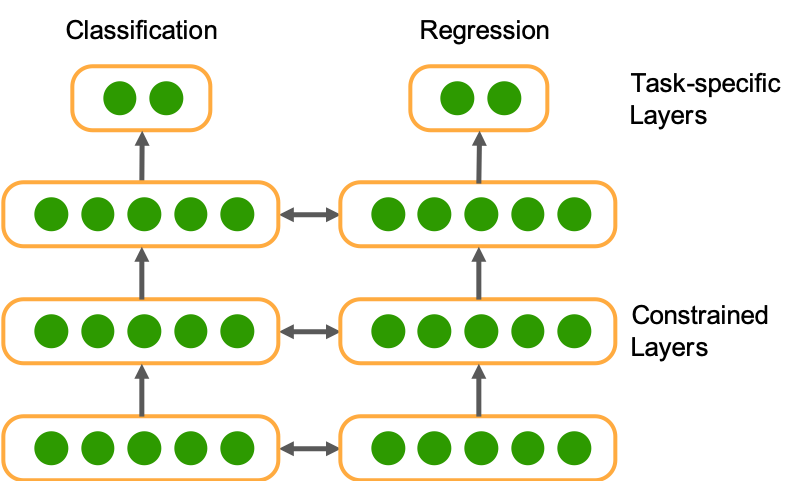
\includegraphics[height=4.2cm]{images/design/multitask_soft.png} \\
    (b) Soft parameter sharing
    \end{minipage}
    \caption{Schematic for two architectures in Multi-Task Learning frameworks}
    \label{fig:mtl}
\end{figure}

Hard parameter sharing architecture greatly reduces the risk of overfitting \cite{baxter1997} and more specifically, the risk of overfitting the shared parameters is an order N smaller than the risk of overfitting the task-specific parameters, where N which represents the number of tasks. I therefore adjust my deep neural network (DNN) classifier to learn on both classification task (mania levels) and regression task (YMRS scores). The joint loss function is defined as the weighted sum of cross entropy loss for classification and the Euclidean loss for regression, as shown in Equation \ref{eq:multi_loss}.

\begin{equation} 
\begin{split}
 \mathcal{L} & = \mathcal{W}_c \mathcal{L}_c + \mathcal{W}_r \mathcal{L}_r \\
             & = \mathcal{W}_c (-\sum_{c=1}^N y_c \log(p_c)) + \mathcal{W}_r (\frac{1}{M} \sum_{i=1}^M \parallel y_r - p_r \parallel ^ 2)
\end{split}
\label{eq:multi_loss}
\end{equation}

where $\mathcal{W}_c$ and $\mathcal{W}_r$ represent the weight for two losses, $y_c$ and $y_r$ are values for two tasks while $p_c$ and $p_r$ are the predicted values, and $N$ is the number of classes and $M$ is the number of samples in the training set.


\chapter{Evaluation}
\label{ch:evaluation}





In this chapter, I evaluate my proposed framework on Bipolar Disorder (BD) recognition. I first describe the baseline system with baseline features against which the proposed framework compares. I then present the experimental results of the Deep Denoising Autoencoders (DDAEs) on audio-visual modalities and document embeddings on text modality respectively, and the final decision is obtained with early fusion strategy, making use of all available modalities. The visualization of reconstructed visual input and embedding space is given for the qualitative analysis. I conclude the chapter with the comparison with other frameworks proposed in AVEC2018. 




\section{Baseline}

For the following experiments, I build a baseline system with Random Forest (RF) classifiers and baseline features presented in AVEC2018 \cite{ringeval2018}.

\subsection{Baseline Features}

As mentioned in Chapter \ref{ch:background} Section \ref{sec:bp-corpus}, the Turkish Audio-Visual Bipolar Disorder (BD) Corpus is recently introduced \cite{cciftcci2018}, which includes pre-partitioned training, development and test sets. The availability of the dataset is upon request while labels for the test set cannot be accessed unless participating in the AVEC2018 challenge. Besides, based on the statistics I obtained on my version of the dataset, the number of recordings in Table \ref{tab:recording_length} cannot be verified \cite{cciftcci2018} as there are only 54 samples without labels in the test partition. The imbalance between three classes is noted that there are more recordings of hypo-mania and mania than those of remission.


\begin{table}[ht]
    \centering
    \caption{Recording statistics for mania patients with different symptoms and healthy controls}
    \small
    \begin{tabular}{l|p{4cm}|p{2cm}|p{2cm}}
         \Xhline{2\arrayrulewidth}
         Diagnosis & Number of recordings in train/dev/test set & Average Time (s) & Standard Deviation \\
         \hline
         Remission & 25/18/NA & 151.9 & 65.4 \\
         \hline
         Hypo-mania & 38/21/NA & 221.1 & 171.4 \\
         \hline
         Mania & 41/21/NA & 276.4 & 246.3 \\
         \Xhline{2\arrayrulewidth}
    \end{tabular}
    \label{tab:recording_length}
\end{table}


Therefore, in the following experiments, I focus my framework on the training and development sets, whose results can be directly compared with the competing frameworks \cite{yang2018, du2018, xing2018, syed2018} in AVEC2018, and then U cross-validate our framework on all the available data for the analysis of generalization.

The baseline features used in AVEC2018 includes MFCC features, eGeMAPS features, and Bag-of-Audio-Words (BoAW) features for acoustic modality, and FAU features and Bag-of-Visual-Words (BoVW) features for visual modality. MFCC features are computed at the frame level while eGeMAPS are computed at speaker turn level that however can be aligned with other modalities given the frame time. FAU features are session-level functionals of action units over each video session, which include the mean, standard-deviation, and the relative position of the maximum. BoAW and BoVW are generated following the BoW technique, described in Chapter \ref{ch:design} Section \ref{sec:fisher}, using frame-level LLDs: MFCC features and FAU features respectively. 


\subsection{Baseline Systems}

With the baseline features available, Random Forest (RF) classifiers are fine-tuned with the following hyperparameters to obtain the optimal frame-level baseline results: the number of trees ($N$), the maximum depth of each tree ($D$) and the maximum portion of features used in each split ($S$). The objective metric used in the tuning process is the unweighted average recall (UAR). Furthermore, the training data of the minority class, remission, is replicated to be balanced with other classes \cite{ringeval2018}.

After fine-tuning and training, the frame-level results for each feature are obtained. To obtain session-level decisions, I apply a simple majority voting strategy to the baseline systems using features other than FAU, which nevertheless does not take into account the global information or temporary information of each video session.  Because of the imbalanced dataset, I measure the performance of baseline systems with recall and precision which respectively describe classifiers completeness and exactness.

\begin{table}[htb]
    \small
    \centering
    \caption{Hyperparameter settings to investigate for Random Forest classifiers}
    \begin{tabular}{l|l}
    \Xhline{2\arrayrulewidth}
        Hyperparameter & Values \\
        \hline
        Number of trees $N$ & \{100, 200, 400, 800\} \\
        Maximum depth of trees $D$ & \{2, 4, 8\} \\
        Maximum features in trees $S$ & \{0.1, 0.2, 0.4\} \\
    \Xhline{2\arrayrulewidth}
    \end{tabular}
    \label{tab:params_rf}
\end{table}


I present the experimental results of the baseline system as Table \ref{tab:baseline}. Of the metrics in Table \ref{tab:baseline}, UAR represents the unweighted average recall, which was used as the primary metric in AVEC2018, UAP represents the unweighted average precision, and F1 represents the F1 score, the harmonic mean of precision and recall: $F_1 = 2 \times \frac{precision \times recall}{precision + recall}$. The symbols F and S in the metric respectively denote frame-level and session-level. 


\begin{table}[htb]
    \small
    \centering
    \caption{Baseline systems with Random Forest classifiers on baseline features}
    \begin{tabular}{l|p{1.5cm}|p{1.9cm}|p{1.5cm}|p{1.5cm}|p{1.5cm}}
    \Xhline{2\arrayrulewidth}
    \hline
         Metric  & MFCC  & eGeMAPS & BoAW & FAU  & BoVW \\
         \hline
         UAR (F) & 0.414 & 0.396 & 0.443 & -     & 0.452 \\
         UAR (S) & 0.413 & 0.455 & \textbf{0.489} & 0.481 & 0.452 \\
         UAP     & 0.410 & 0.370 & 0.439 & \textbf{0.528} & 0.445 \\
         F1      & 0.411 & 0.408 & 0.463 & \textbf{0.503} & 0.448 \\
    \hline
    \Xhline{2\arrayrulewidth}
    \end{tabular}
    \label{tab:baseline}
\end{table}


As shown in Table \ref{tab:baseline}, BoAW-based baseline system outperforms others with an UAR at 0.489 while MFCC-based baseline the UAR is the lowest at only 0.413. It is noticeable that the baseline using FAU features has the second highest UAR score along with the highest UAP, resulting in the highest F1 score. The BoAW-based and FAU-based systems are selected as the baseline for the following experiments.





\section{Audio-Visual Modalities}

To validate the feature learning of audio-visual modalities, the proposed Deep Denoising Autoencoders (DDAEs) are evaluated with the performance in the supervised learning task, BD classification. As the number of Gaussians (16 or 32) in Fisher Vectors (FVs) is investigated, there would be 36 hyperparameter settings for just the Unimodal DDAE architectures. Thus I focus on the hyperparameters of DDAEs, whose results are based on the better-performing Fisher Vector, using either 16 or 32 kernels in the Gaussian Mixture Models. Furthermore, to solely evaluate the latent representations of DDAEs and the FVs, the classification performance is measured with the same fine-tuned Random Forest (RF) classifiers as the baseline system. The complete experimental results are attached in Appendix \ref{sec:DDAE_full}. As Chapter \ref{ch:design} Section \ref{sec:DDAE}, the Unimodal DDAEs (uni-DDAEs), Bimodal DDAEs (bi-DDAEs), and Multimodal DDAEs (multi-DDAEs) are individually evaluated in the following subsections.

\subsection{Assessment of Unimodal Feature Learning}

I first present the experimental results for unimodal feature learning in Table \ref{tab:unimodal_res}, in which DDAEs are trained on unimodal data: facial landmarks, MFCC features or eGeMAPS features. A Monte Carlo permutation test is additionally implemented for the following experiments to evaluate the probability that the difference between baseline systems and proposed systems occurs by random chance. As there are 60 samples in the development set, the number of random permutations is pre-fixed to 5000 instead of $2^{60}$.


\begin{table}[htb]
    \small
    \centering
    \caption{Comparison of proposed Unimodal DDAE architectures (selected experimental results). The best performance is in \textbf{bold} for each metric and the baseline results are attached.}
    \begin{tabular}{l|l|p{1.25cm}|l|p{1.2cm}|l|l|l}
    \Xhline{2\arrayrulewidth}
        Index & Acoustic feature & Hidden ratio & Noise & GMM kernel & UAR & UAP & F1 \\
        \hline
        (1)  & Landmarks & 0.4 & 0.1 & 16 & 0.582 & 0.590 & 0.586 \\
        (2)  & Landmarks & 0.4 & 0.2 & 32 & \textbf{0.624} & \textbf{0.692} & \textbf{0.656} \\
        (3)  & Landmarks & 0.4 & 0.4 & 32 & 0.614 & 0.622 & 0.618 \\
        (4)  & Landmarks & 0.5 & 0.1 & 16 & 0.585 & 0.628 & 0.606 \\
        (5)  & Landmarks & 0.5 & 0.2 & 32 & 0.606 & 0.635 & 0.620 \\
        (6)  & Landmarks & 0.5 & 0.4 & 32 & 0.611 & 0.620 & 0.615 \\
        \hline
        (7)  & MFCC & 0.4 & 0.1 & 32 & \textbf{0.587} & \textbf{0.611} & \textbf{0.599} \\
        (8)  & MFCC & 0.4 & 0.2 & 32 & 0.542 & 0.562 & 0.552 \\
        (9)  & MFCC & 0.4 & 0.4 & 16 & 0.521 & 0.562 & 0.541 \\
        (10) & MFCC & 0.5 & 0.1 & 16 & 0.550 & 0.575 & 0.562 \\
        (11) & MFCC & 0.5 & 0.2 & 32 & 0.561 & 0.607 & 0.583 \\
        (12) & MFCC & 0.5 & 0.4 & 16 & 0.545 & 0.585 & 0.564 \\
        \hline
        (13) & eGeMAPS & 0.4 & 0.1 & 16 & 0.561 & 0.591 & 0.576 \\
        (14) & eGeMAPS & 0.4 & 0.2 & 32 & 0.524 & 0.532 & 0.528 \\
        (15) & eGeMAPS & 0.4 & 0.4 & 32 & 0.511 & 0.563 & 0.536 \\
        (16) & eGeMAPS & 0.5 & 0.1 & 32 & \textbf{0.632} & \textbf{0.654} & \textbf{0.637} \\
        (17) & eGeMAPS & 0.5 & 0.2 & 32 & 0.590 & 0.619 & 0.604 \\
        (18) & eGeMAPS & 0.5 & 0.4 & 32 & 0.563 & 0.585 & 0.574 \\
        \hline
        & \multicolumn{4}{l|}{Baseline (BoAW)} & 0.489 & 0.439 & 0.463 \\
        & \multicolumn{4}{l|}{Baseline (FAU)} & 0.481 & 0.528 & 0.503 \\
    \Xhline{2\arrayrulewidth}
    \end{tabular}
    \label{tab:unimodal_res}
\end{table}


In Table \ref{tab:unimodal_res}, the results show an improvement from the baseline system. Specifically, for facial landmarks, the best-performing uni-DDAE reaches up to 0.624 UAR with 0.658 F1 score ((2) in Table \ref{tab:unimodal_res}) and for eGeMAPS features, the uni-DDAEs obtain a higher UAR at 0.632 with 0.637 F1 score ((16) in Table \ref{tab:unimodal_res}). On the other hand, UAR for uni-DDAEs using MFCC features is lower than other uni-DDAEs at only 0.587 but higher than the best-performing baseline as (7) seen in Table \ref{tab:unimodal_res}. With respect to uni-DDAEs and baseline systems using same features, (7) performs significantly between than the baseline using MFCC ($p = 0.0002 < 0.001$) but (16) does not outperform the baseline using eGeMAPS significantly ($p = 0.4459 > 0.1$).

It is clear that a compact size benefits latent representations for facial landmarks because the DDAEs with hidden ratio 0.4 (21-dimensional representations) show better performance than those with hidden ratio 0.5 (34-dimensional representations). While the smaller hidden ratio for DDAEs using eGeMAPS features affects the performance negatively, the hidden ratio seems to have little impact on the performance of DDAEs using MFCC features. 

The noise appended to the input forces the autoencoders to learn more robust features \cite{vincent2008}, which can be validated in DDAEs with facial landmarks as 0.2 noise leads to a higher F1 score than 0.1 noise. Nevertheless, to the acoustic features, more noise causes F1 score to decrease.

To the acoustic features, eGeMAPS features demonstrate a better performance over MFCC features in uni-DDAEs. The best-performing RF classifiers ((7) and (16) in Table \ref{tab:unimodal_res}) show a performance gap of 0.045 in UAR and 0.038 in F1 score but they fail to significantly differ from each other with $p = 0.16 > 0.1$


\begin{figure}
    \centering
    \small
    \begin{minipage}[c]{0.31\linewidth}
    \centering
    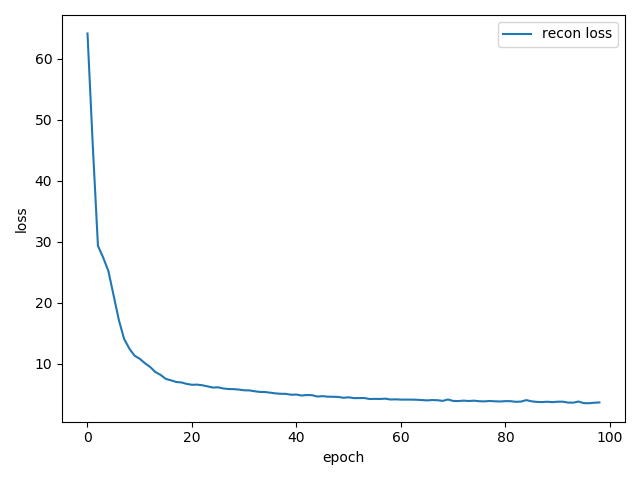
\includegraphics[width=\textwidth]{images/results/unimodal_landmark_hidden040_batch1024_epoch100_noise02.png} \\
    Facial Landmarks
    \end{minipage}
    \begin{minipage}[c]{0.31\linewidth}
    \centering
    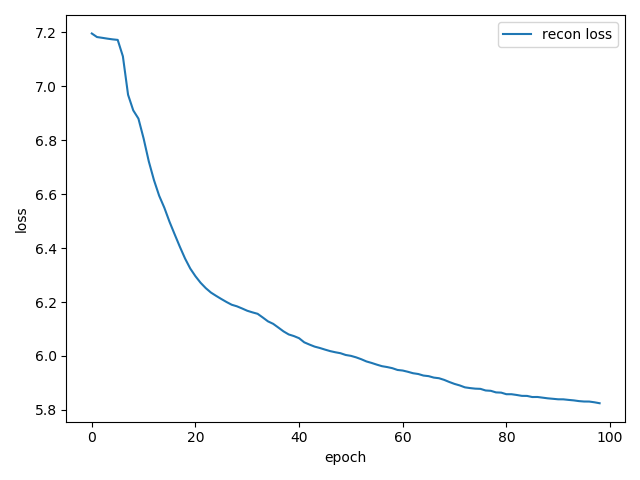
\includegraphics[width=\textwidth]{images/results/unimodal_mfcc_hidden040_batch1024_epoch100_noise01.png} \\
    MFCC
    \end{minipage}
    \begin{minipage}[c]{0.31\linewidth}
    \centering
    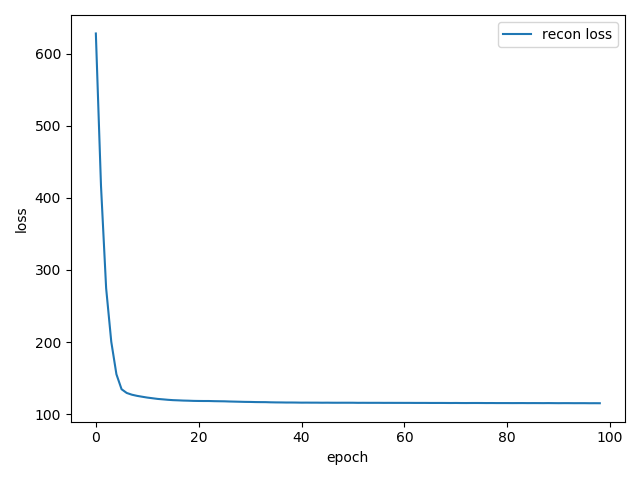
\includegraphics[width=\textwidth]{images/results/unimodal_egemaps_hidden050_batch1024_epoch100_noise01.png} \\
    eGeMAPS
    \end{minipage}
    \caption{Loss during training for Unimodal DDAE}
    \label{fig:loss_unimodal}
\end{figure}

The reconstruction loss during the training processing is visualized for the best-performing uni-DDAEs ((2), (7) and (16) in Table \ref{tab:unimodal_res}) using different features as Figure \ref{fig:loss_unimodal}. As discussed in Chapter \ref{ch:design} Section \ref{sec:DDAE}, the loss function is set the mean squared error (MSE) instead of binary cross-entropy (BCE) as I find that with BCE, the loss cannot be minimized in the training and the latent representations prove meaningless in the classification. Although three uni-DDAEs succeed to minimize the reconstruction loss, it is worthy to notice the different ranges of loss values, which is discussed in the bimodal feature learning.

The full version of experimental results for uni-DDAEs refers to \ref{tab:unimodal_res_full}.




\subsection{Assessment of Bimodal Feature Learning}

In the bimodal feature learning, the visual modality is fixed to facial landmarks and the acoustic modality is investigated on either MFCC features or eGeMAPS features. As seen in Table \ref{tab:bimodal_res}, bi-DDAEs with MFCC as acoustic feature generally have better performance than those with eGeMAPS. When compared to the best-performing uni-DDAEs with facial landmarks and MFCC, a performance gain is observed in bi-DDAEs with MFCC that the joint representations across two modalities demonstrate more discriminative for BD recognition. However, bi-DDAEs with eGeMAPS show a performance drop instead that the F1 score is lower than either uni-DDAE using acoustic or visual modality. This finding may explained with the loss during training for uni-DDAEs (Figure \ref{fig:loss_unimodal}) and bi-DDAEs (Figure \ref{fig:loss_bimodal}). As displayed in Figure \ref{fig:loss_unimodal}, the loss for facial landmarks decreases to approximately 5.0, within the same scale of MFCC features, while the loss for eGeMAPS features starts at more than 600.0 and is finally minimized at 115.0, which is much larger than the scale for other two features. Therefore, in the bi-DDAEs with eGeMAPS, the acoustic loss still starts at a high value and causes the joint loss higher than the visual loss. More specifically, the acoustic loss is reduced to around 83.4 while the visual loss to around 27.0. On the other hand, the acoustic and visual loss in bi-DDAEs using MFCC decline with the same pattern and end at approximately 10.3 and 6.3 respectively.

\begin{figure}
    \centering
    \small
    \begin{minipage}[c]{0.48\linewidth}
    \centering
    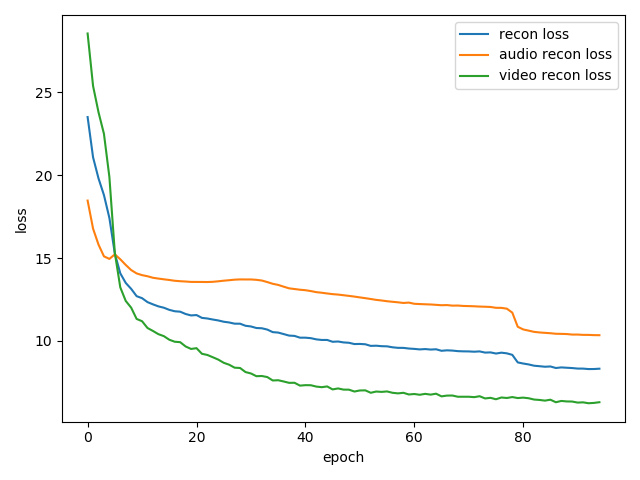
\includegraphics[width=\textwidth]{images/results/bimodal_aligned_mfcc_hidden040_batch1024_epoch100_noise01.png} \\
    MFCC
    \end{minipage}
    \begin{minipage}[c]{0.48\linewidth}
    \centering
    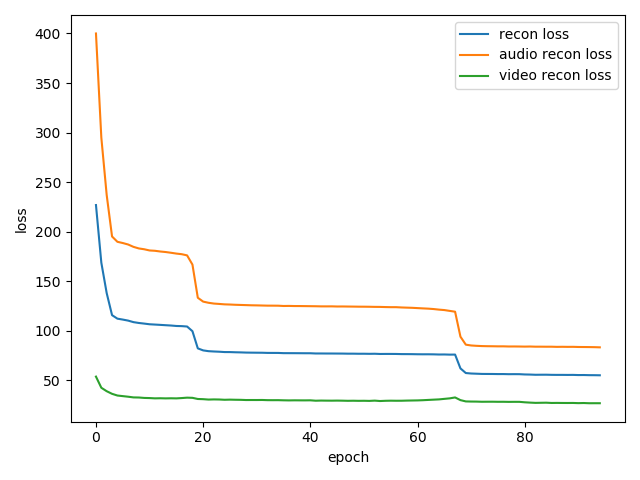
\includegraphics[width=\textwidth]{images/results/bimodal_aligned_egemaps_hidden050_batch1024_epoch100_noise01.png} \\
    eGeMAPS
    \end{minipage}
    \caption{Loss during training for Bimodal DDAE}
    \label{fig:loss_bimodal}
\end{figure}

In addition to the better performance of bi-DDAEs, the kernels of GMMs has proven a considerable impact on the classification, which in bi-DDAEs are mostly 32. Nonetheless, the bi-DDAE (1) in Table \ref{tab:bimodal_res} with 16 GMM kernels has an UAR at 0.492 and F1 score at 0.473, much lower than the same setting with 32 GMM kernels (Table \ref{tab:bimodal_res_full}). 

The size of latent representations affects the performance the same way as the uni-DDAEs on MFCC and eGeMAPS that bi-DDAEs on MFCC favour a smaller hidden ratio while those on eGeMAPS favour a larger hidden ratio. In terms of noise, much noise (more than 0.1) is observed to hurt the performance. It is worth pointing out that bi-DDAE (1) in Table \ref{tab:bimodal_res} slightly outperforms the framework proposed by \cite{syed2018} in AVEC2018.

The full version of experimental results for Bimodal DDAEs refers to \ref{tab:bimodal_res_full}.

\begin{table}[htb]
    \small
    \centering
    \caption{Comparison of proposed Bimodal DDAE architectures (selected experimental results). The best performance is in \textbf{bold} for each metric, and the baseline results and best-performing results for Unimodal DDAEs are attached.}
    \begin{tabular}{l|p{1.8cm}|p{1.25cm}|l|p{1.2cm}|l|l|l}
    \Xhline{2\arrayrulewidth}
        Index & Acoustic feature & Hidden ratio & Noise & GMM kernel & UAR & UAP & F1 \\
        \hline
        (1)  & MFCC  & 0.4 & 0.1 & 32 & \textbf{0.656} & \textbf{0.677} & \textbf{0.666} \\
        (2)  & MFCC  & 0.4 & 0.2 & 16 & 0.632 & 0.644 & 0.638 \\
        (3)  & MFCC  & 0.4 & 0.4 & 32 & 0.447 & 0.462 & 0.454 \\
        (4)  & MFCC  & 0.5 & 0.1 & 32 & 0.505 & 0.524 & 0.514 \\
        (5)  & MFCC  & 0.5 & 0.2 & 32 & 0.489 & 0.586 & 0.533 \\
        (6)  & MFCC  & 0.5 & 0.4 & 32 & 0.545 & 0.561 & 0.553 \\
        \hline
        (7)  & eGeMAPS & 0.4 & 0.1 & 32 & 0.566 & 0.569 & 0.567 \\
        (8)  & eGeMAPS & 0.4 & 0.2 & 32 & 0.516 & 0.600 & 0.555 \\
        (9)  & eGeMAPS & 0.4 & 0.4 & 32 & 0.511 & 0.538 & 0.524 \\
        (10) & eGeMAPS & 0.5 & 0.1 & 16 & \textbf{0.566} & \textbf{0.611} & \textbf{0.587} \\
        (11) & eGeMAPS & 0.5 & 0.2 & 16 & 0.479 & 0.497 & 0.488 \\
        (12) & eGeMAPS & 0.5 & 0.4 & 32 & 0.519 & 0.607 & 0.560 \\
        \hline
        & \multicolumn{4}{l|}{Baseline (BoAW)} & 0.489 & 0.439 & 0.463 \\
        & \multicolumn{4}{l|}{Baseline (FAU)} & 0.481 & 0.528 & 0.503 \\
        \hline
        & \multicolumn{4}{l|}{Best Unimodal DDAE (Landmarks)} & 0.624 & 0.692 & 0.656 \\
        & \multicolumn{4}{l|}{Best Unimodal DDAE (MFCC)} & 0.587 & 0.611 & 0.599 \\
        & \multicolumn{4}{l|}{Best Unimodal DDAE (eGeMAPS)} & 0.632 & 0.654 & 0.637 \\
    \Xhline{2\arrayrulewidth}
    \end{tabular}
    \label{tab:bimodal_res}
\end{table}



\subsection{Assessment of Multimodal Feature Learning}

For multimodal feature learning, a total of five modalities are input into the multi-DDAEs including acoustic features (either MFCC or eGeMAPS), facial landmarks, eye gaze, head pose, and action units. As shown in Table \ref{tab:multimodal_res}, multi-DDAE (1) using MFCC features performs the best, with 0.656 UAR and 0.667 F1 score, but it fails to outperform the best-performing bi-DDAE on the same features because UAR are 0.656 for both models and $p = 0.69 >> 0.1$ in the permutation test. However, a small increase is obtained in other multi-DDAEs using MFCC features when compared with bi-DDAEs with the same hyperparameter setting. This demonstrates the \textit{complementarity} of multi-modal data that modality-specific information has been appended to the system by addition modality: eye gaze, head pose, and action units. Nonetheless, it is also noticeable that only multi-DDAE (2) in Table \ref{tab:multimodal_res} shows a decrease in all metrics compared with bi-DDAE (2) in Table \ref{tab:bimodal_res}. 

For eGeMAPS features, there is a considerable gain in UAR of multi-DDAEs when compared with bi-DDAEs. The best-performing bi-DDAE with eGeMAPS has an UAR of 0.566 while multi-DDAE (10) in Table \ref{tab:multimodal_res} reaches an UAR of 0.622 (0.056 higher). and it performs significantly better than the former with $p = 0.05$ in the permutation test.

The multi-DDAEs follow the same pattern as bi-DDAEs in the hyperparameter, hidden ratio, that multi-DDAEs using MFCC tend to perform better with a more compact size of the latent representation. The same pattern is found in another hyperparameter, noise, that much noise negatively affects the performance, such as a dramatic drop of 0.08 in F1 score when compared (8) with (9).

\begin{figure}
    \centering
    \small
    \begin{minipage}[c]{0.48\linewidth}
    \centering
    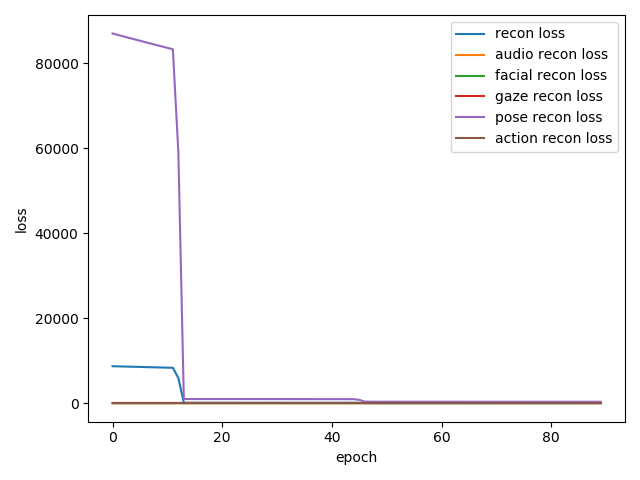
\includegraphics[width=\textwidth]{images/results/multimodal_aligned_mfcc_hidden040_batch1024_epoch100_noise01_full.png}
    \end{minipage}
    \begin{minipage}[c]{0.48\linewidth}
    \centering
    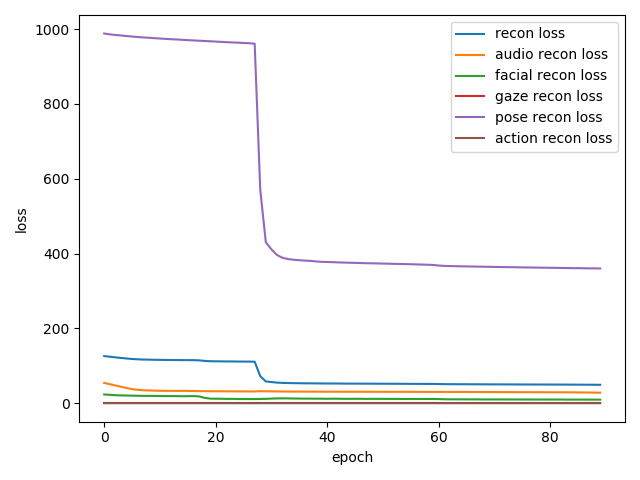
\includegraphics[width=\textwidth]{images/results/multimodal_aligned_egemaps_hidden050_batch1024_epoch100_noise01_full.png}
    \end{minipage}
    \begin{minipage}[c]{0.48\linewidth}
    \centering
    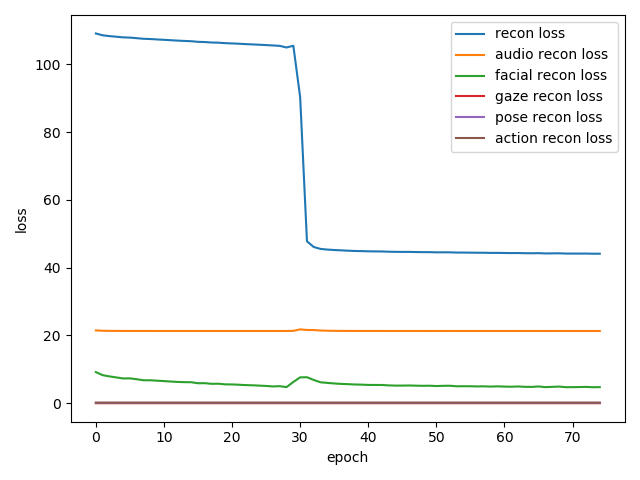
\includegraphics[width=\textwidth]{images/results/multimodal_aligned_mfcc_hidden040_batch1024_epoch100_noise01.png} \\
    MFCC
    \end{minipage}
    \begin{minipage}[c]{0.48\linewidth}
    \centering
    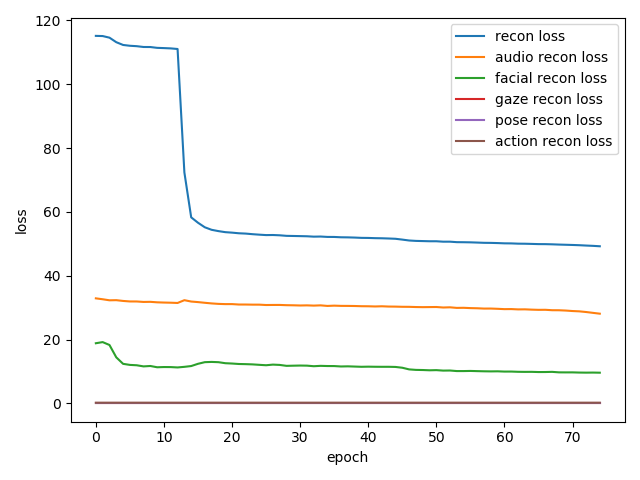
\includegraphics[width=\textwidth]{images/results/multimodal_aligned_egemaps_hidden050_batch1024_epoch100_noise01.png} \\
    eGeMAPS
    \end{minipage}
    \caption{Loss during training for Multimodal DDAE (The reconstruction loss for modality head pose is removed in the second-row graphs)}
    \label{fig:loss_multimodal}
\end{figure}

With the visualization of reconstruction loss in multi-DDAEs (1) and (10) in Table \ref{tab:multimodal_res}, some findings can help to explain little improvement of multi-DDAEs using MFCC. In Figure \ref{fig:loss_multimodal}, the two images on the upper row show the reconstruction loss of all five modalities during training and the two images on the lower row focus on the modalities except head pose, which is preset to zero. Head pose is demonstrated difficult to be reconstructed via the multi-DDAEs as the head pose loss is relatively larger than other modalities. 

The full version of experimental results for Multimodal DDAEs refers to \ref{tab:multimodal_res_full}.



\begin{table}[htb]
    \small
    \centering
    \caption{Comparison of proposed Multimodal DDAE architectures (selected experimental results). The best performance is in \textbf{bold} for each metric, and the baseline results and best-performing results for previous DDAEs are attached.}
    \begin{tabular}{l|p{1.8cm}|p{1.25cm}|l|p{1.2cm}|l|l|l}
    \Xhline{2\arrayrulewidth}
        Index & Acoustic feature & Hidden ratio & Noise & GMM kernel & UAR & UAP & F1 \\
        \hline
        (1)  & MFCC  & 0.4 & 0.1 & 32 & \textbf{0.656} & \textbf{0.678} & \textbf{0.667} \\
        (2)  & MFCC  & 0.4 & 0.2 & 32 & 0.566 & 0.573 & 0.569 \\
        (3)  & MFCC  & 0.4 & 0.4 & 16 & 0.569 & 0.593 & 0.581 \\
        (4)  & MFCC  & 0.5 & 0.1 & 16 & 0.597 & 0.596 & 0.596 \\
        (5)  & MFCC  & 0.5 & 0.2 & 32 & 0.569 & 0.578 & 0.573 \\
        (6)  & MFCC  & 0.5 & 0.4 & 16 & 0.569 & 0.697 & 0.627 \\
        \hline
        (7)  & eGeMAPS & 0.4 & 0.1 & 16 & 0.603 & 0.717 & 0.655 \\
        (8)  & eGeMAPS & 0.4 & 0.2 & 32 & 0.585 & 0.590 & 0.587 \\
        (9)  & eGeMAPS & 0.4 & 0.4 & 16 & 0.489 & 0.514 & 0.501 \\
        (10) & eGeMAPS & 0.5 & 0.1 & 32 & \textbf{0.622} & \textbf{0.665} & \textbf{0.642} \\
        (11) & eGeMAPS & 0.5 & 0.2 & 16 & 0.574 & 0.570 & 0.572 \\
        (12) & eGeMAPS & 0.5 & 0.4 & 16 & 0.484 & 0.536 & 0.507 \\
        \hline
        & \multicolumn{4}{l|}{Baseline (BoAW)} & 0.489 & 0.439 & 0.463 \\
        & \multicolumn{4}{l|}{Baseline (FAU)} & 0.481 & 0.528 & 0.503 \\
        \hline
        & \multicolumn{4}{l|}{Best Unimodal DDAE (Landmarks)} & 0.624 & 0.692 & 0.656 \\
        & \multicolumn{4}{l|}{Best Unimodal DDAE (MFCC)} & 0.587 & 0.611 & 0.599 \\
        & \multicolumn{4}{l|}{Best Unimodal DDAE (eGeMAPS)} & 0.632 & 0.654 & 0.637 \\
        \hline
        & \multicolumn{4}{l|}{Best Bimodal DDAE (MFCC)} & 0.656 & 0.677 & 0.666 \\
        & \multicolumn{4}{l|}{Best Bimodal DDAE (eGeMAPS)} & 0.566 & 0.611 & 0.587 \\
    \Xhline{2\arrayrulewidth}
    \end{tabular}
    \label{tab:multimodal_res}
\end{table}


\subsection{Visualization}

To evaluate the denoising effect of bi-DDAEs and multi-DDAEs, the facial landmarks are selected in the visualization of the reconstructed input. Figure \ref{fig:reconstruction_biDDAE} displays the reconstruction in bi-DDAEs at two specific frames and the images of the interviewee are reserved for better illustration. It is clear that the bi-DDAE on eGeMAPS ((10) in Table \ref{tab:bimodal_res}) performs better at the denoising that the reconstructed facial landmarks are perceived closer to the original input. The bi-DDAE on MFCC ((1) in Table \ref{tab:bimodal_res}), on the other hand, does not reconstruct the facial landmarks properly but the spatial distribution is restored via the decoder part.

\begin{figure}[htb]
    \centering
    \small
    \begin{minipage}[c]{0.42\linewidth}
    \centering
    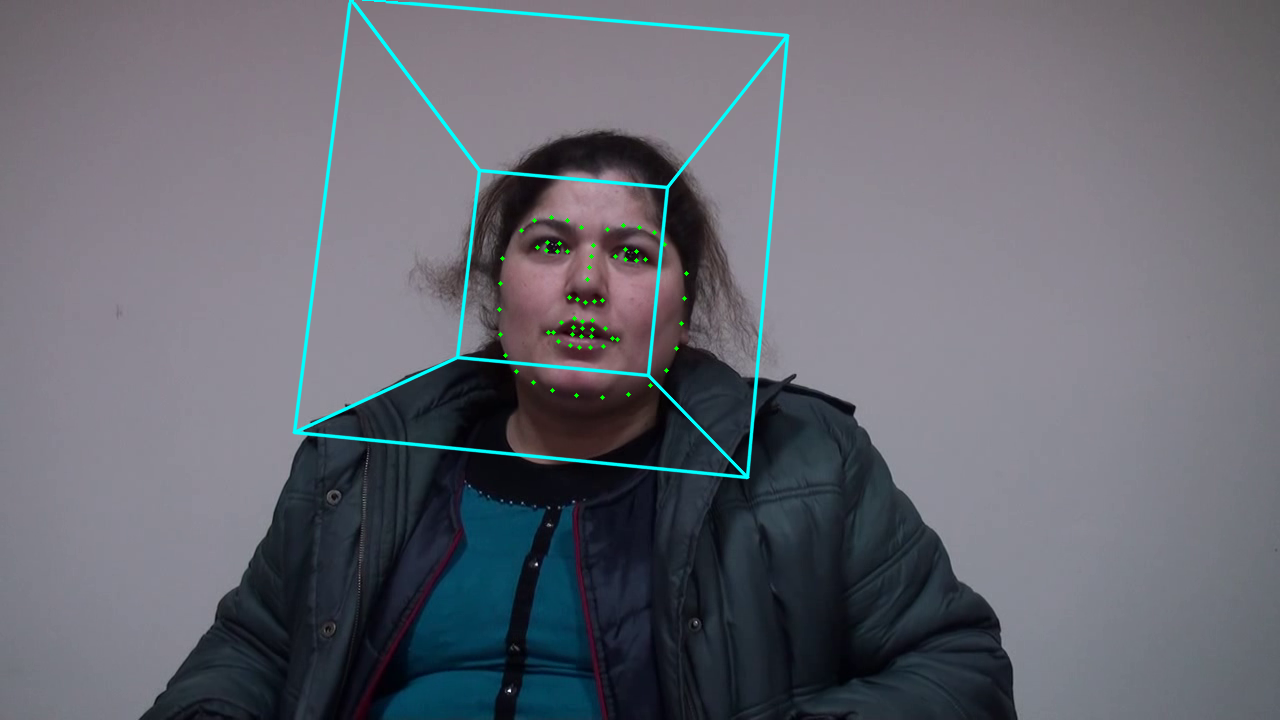
\includegraphics[width=\textwidth]{images/facial/frame_45_face_0.png} \\
    (a) original input at frame 45 (without noise)
    \end{minipage}
    \begin{minipage}[c]{0.42\linewidth}
    \centering
    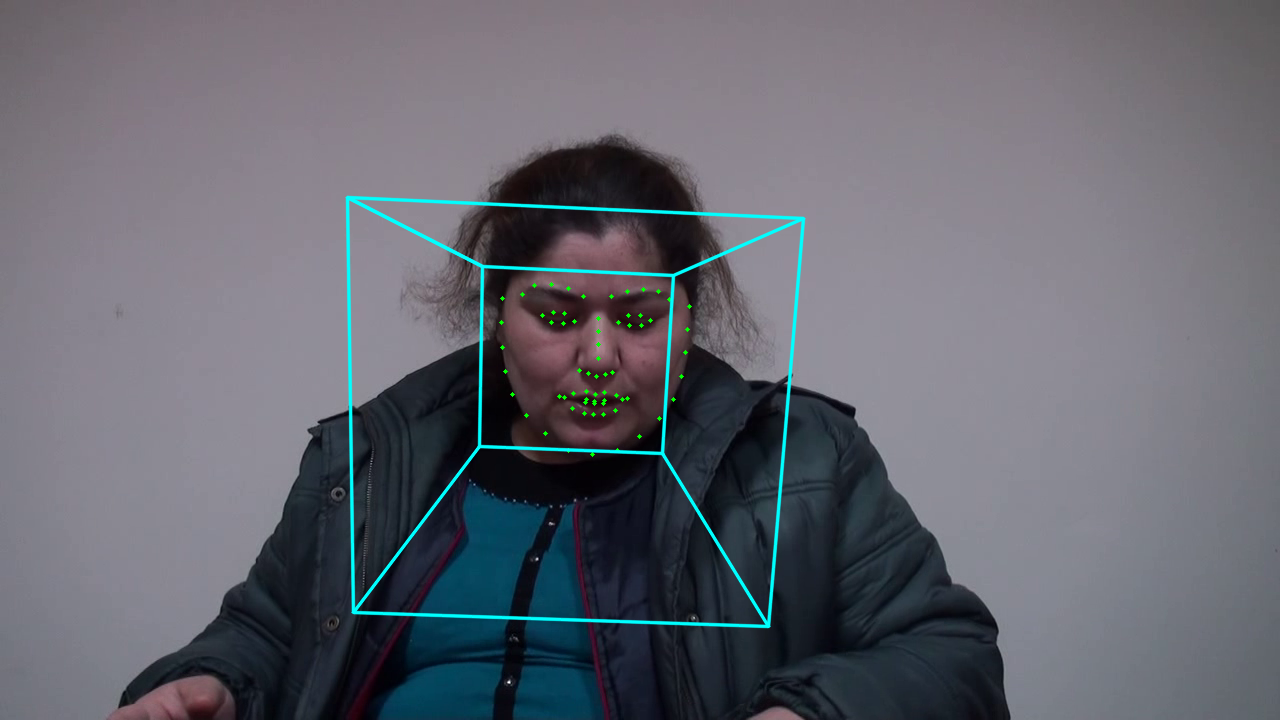
\includegraphics[width=\textwidth]{images/facial/frame_285_face_0.png} \\
    (b) original input at frame 285 (without noise)
    \end{minipage}
    \\
    \begin{minipage}[c]{0.42\linewidth}
    \centering
    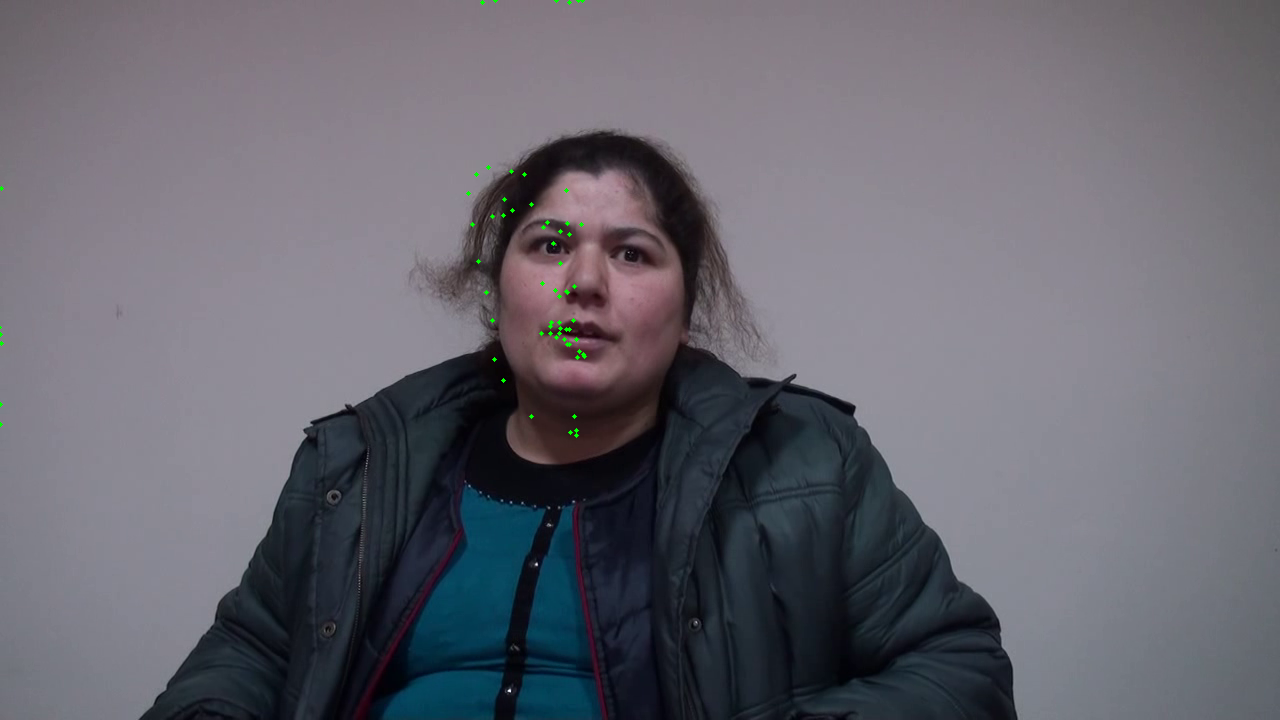
\includegraphics[width=\textwidth]{images/facial/recons_45_face_0_biDDAE_mfcc.png} \\
    (c) reconstructed input at frame 45 from (1) in Table \ref{tab:bimodal_res}
    \end{minipage}
    \begin{minipage}[c]{0.42\linewidth}
    \centering
    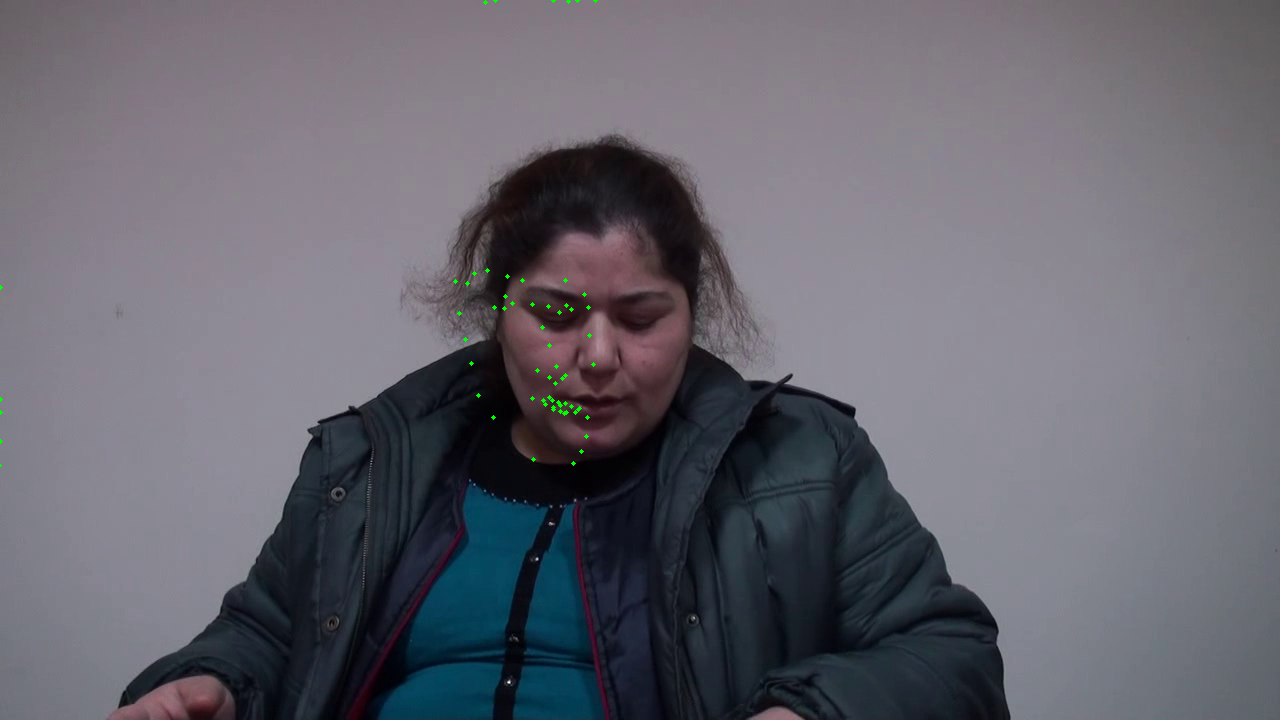
\includegraphics[width=\textwidth]{images/facial/recons_285_face_0_biDDAE_mfcc.png} \\
    (d) reconstructed input at frame 285 from (1) in Table \ref{tab:bimodal_res}
    \end{minipage}
    \\
    \begin{minipage}[c]{0.42\linewidth}
    \centering
    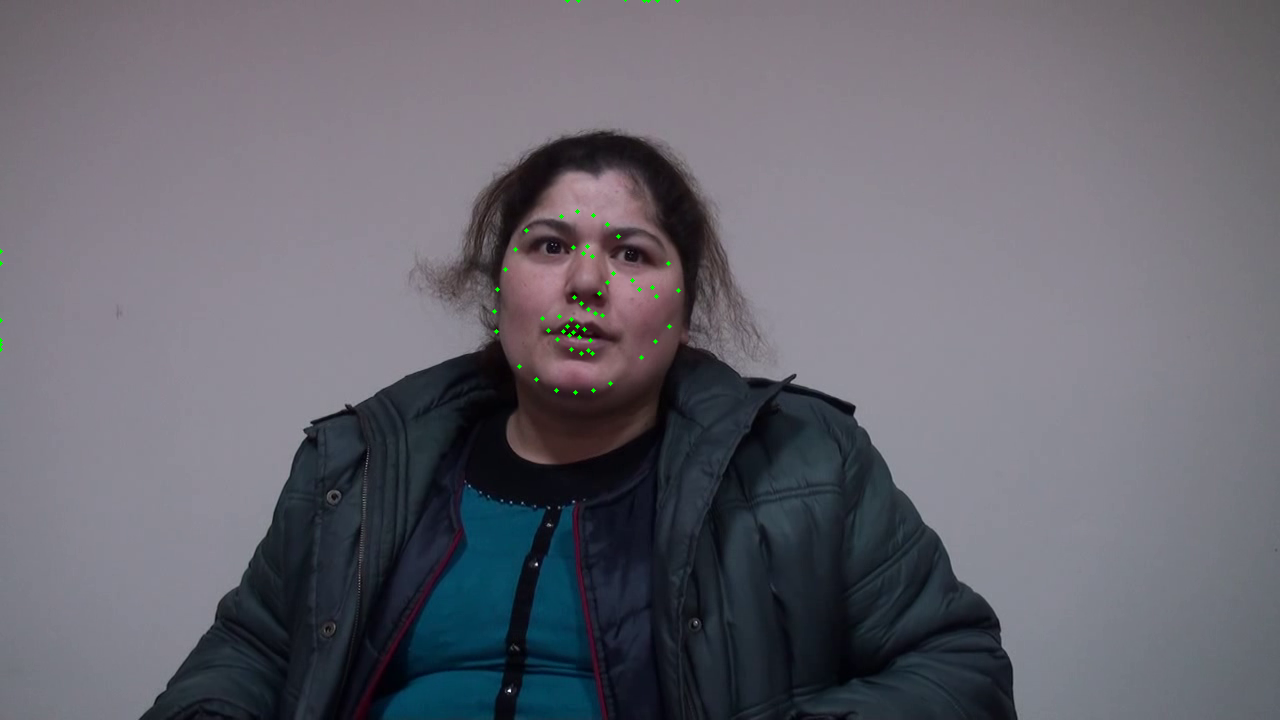
\includegraphics[width=\textwidth]{images/facial/recons_45_face_0_biDDAE_egemaps.png} \\
    (e) reconstructed input at frame 45 from (10) in Table \ref{tab:bimodal_res}
    \end{minipage}
    \begin{minipage}[c]{0.42\linewidth}
    \centering
    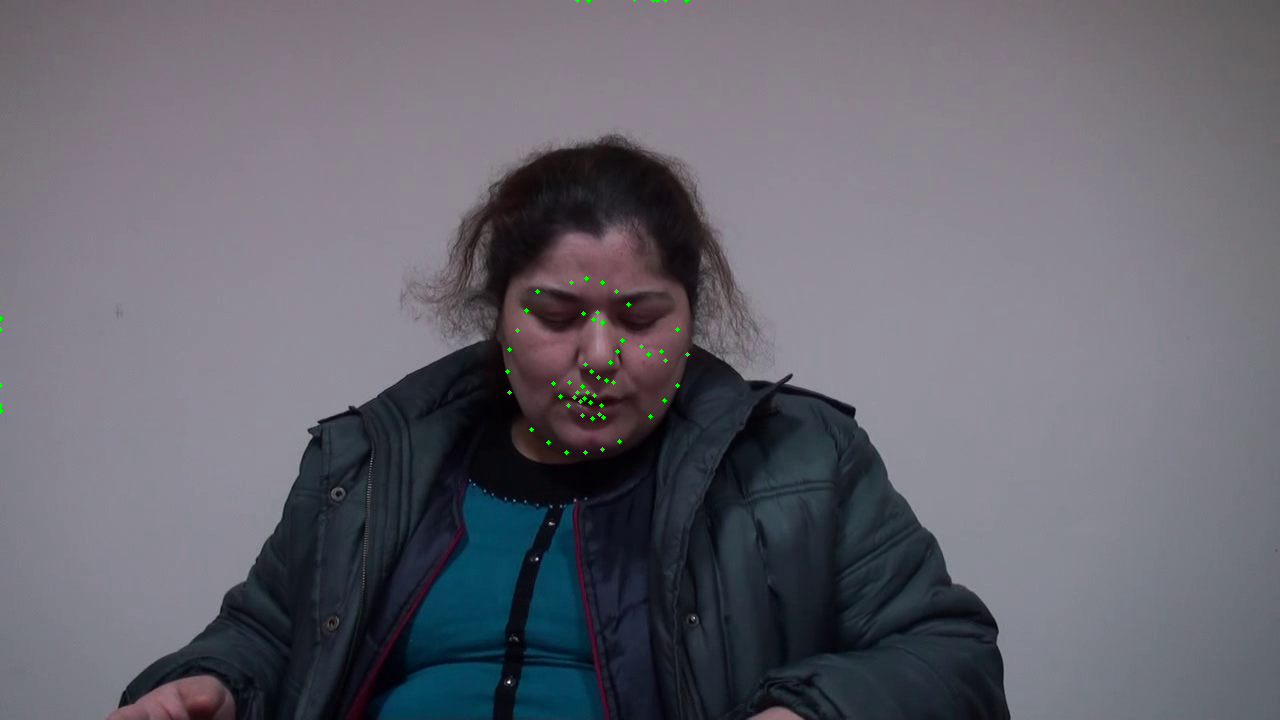
\includegraphics[width=\textwidth]{images/facial/recons_285_face_0_biDDAE_egemaps.png} \\
    (f) reconstructed input at frame 285 from (10) in Table \ref{tab:bimodal_res}
    \end{minipage}
    \caption{Reconstruction of facial landmarks in Bimodal DDAEs from noisy input}
    \label{fig:reconstruction_biDDAE}
\end{figure}

Because the head pose is relatively difficult to reconstruct as seen from Figure \ref{fig:loss_multimodal}, the reconstructed facial landmarks and head pose are visualized for multi-DDAEs in Figure \ref{fig:reconstruction_multiDDAE}. (c) and (d) in Figure \ref{fig:reconstruction_multiDDAE} demonstrates that the reconstruction of these two modalities is not intuitively convincing and the involvement of more modalities makes it more difficult to reconstruct one single modality. Moreover, the head pose in (a) and (b) is different from each other while the reconstructions (c) and (d) approximately show no difference. Similar conclusions could be drawn to multi-DDAEs on eGeMAPS ((10) in Table \ref{tab:multimodal_res}). 

\begin{figure}[htb]
    \centering
    \small
    \begin{minipage}[c]{0.42\linewidth}
    \centering
    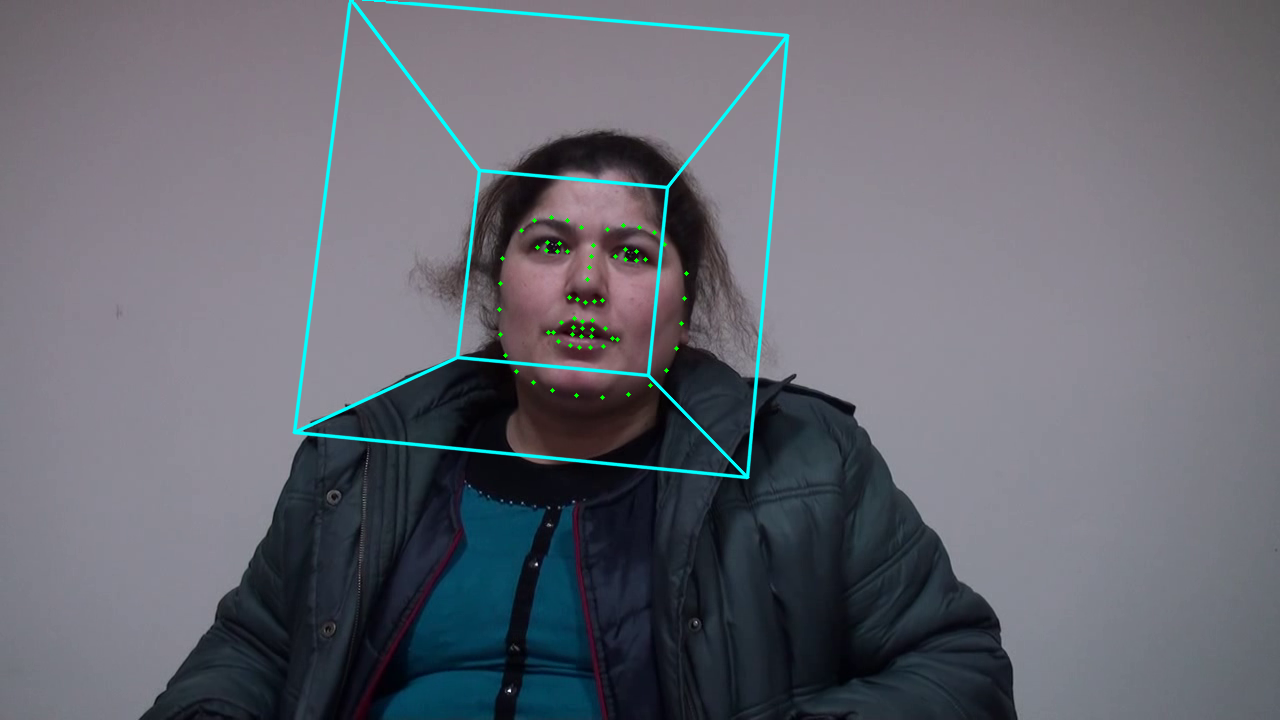
\includegraphics[width=\textwidth]{images/facial/frame_45_face_0.png} \\
    (a) original input at frame 45 (without noise)
    \end{minipage}
    \begin{minipage}[c]{0.42\linewidth}
    \centering
    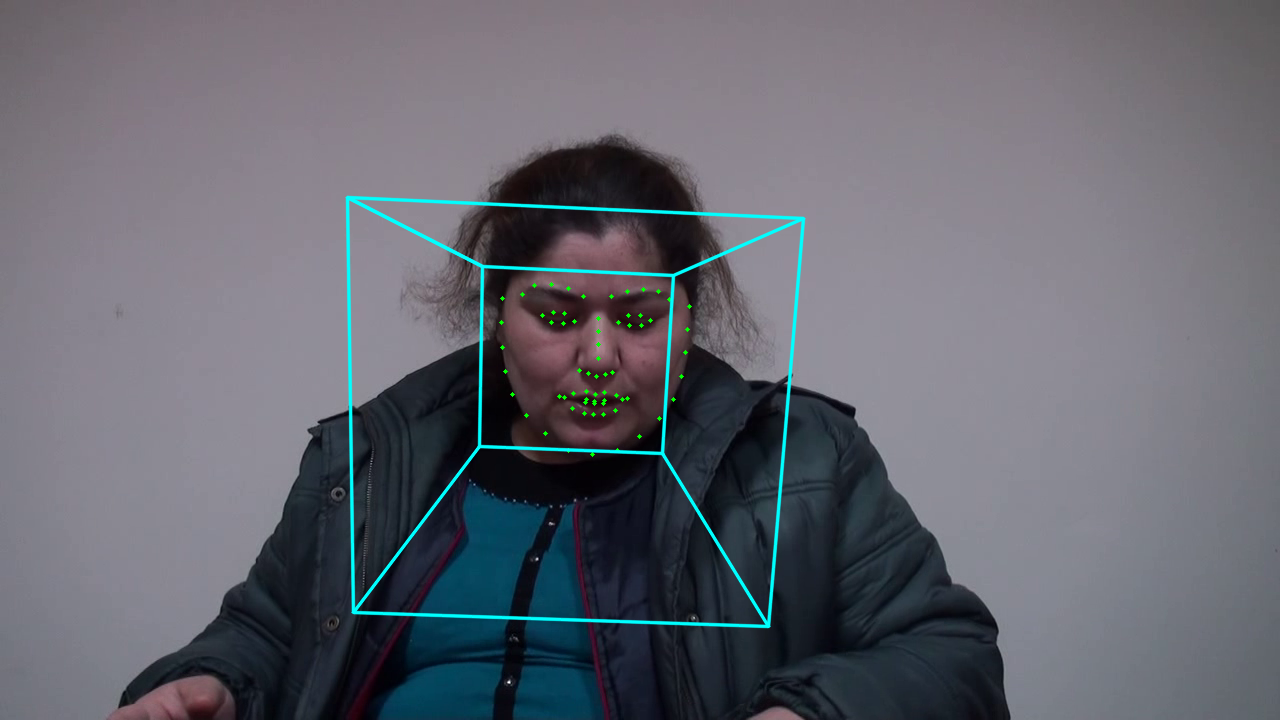
\includegraphics[width=\textwidth]{images/facial/frame_285_face_0.png} \\
    (b) original input at frame 285 (without noise)
    \end{minipage}
    \\
    \begin{minipage}[c]{0.42\linewidth}
    \centering
    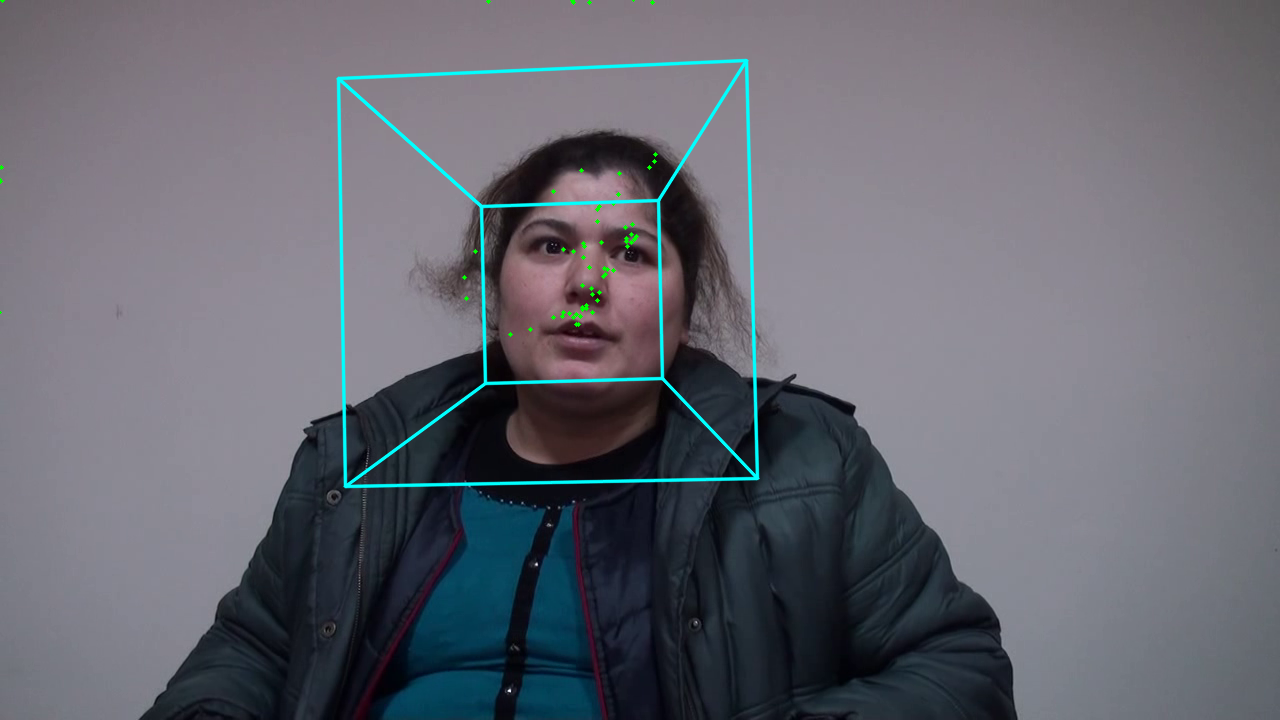
\includegraphics[width=\textwidth]{images/facial/recons_45_face_0_multiDDAE_mfcc.png} \\
    (c) reconstructed input at frame 45 from (1) in Table \ref{tab:multimodal_res}
    \end{minipage}
    \begin{minipage}[c]{0.42\linewidth}
    \centering
    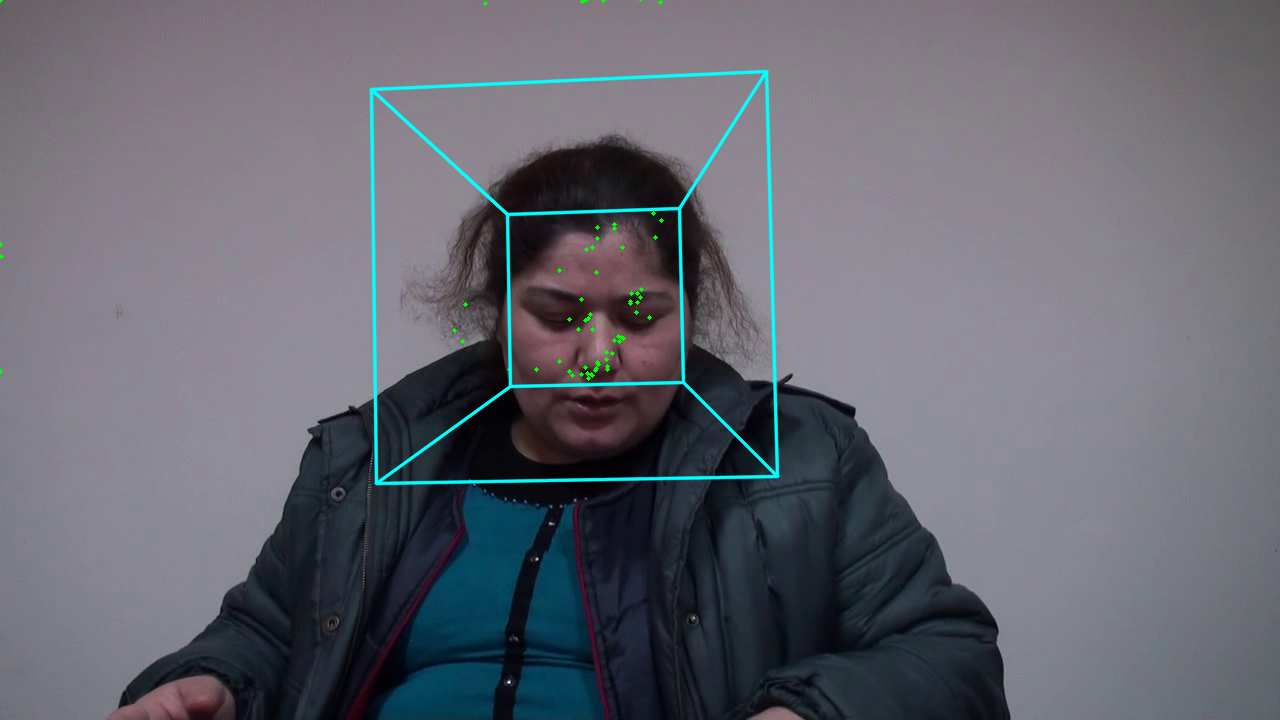
\includegraphics[width=\textwidth]{images/facial/recons_285_face_0_multiDDAE_mfcc.png} \\
    (d) reconstructed input at frame 285 from (1) in Table \ref{tab:multimodal_res}
    \end{minipage}
    \\
    \begin{minipage}[c]{0.42\linewidth}
    \centering
    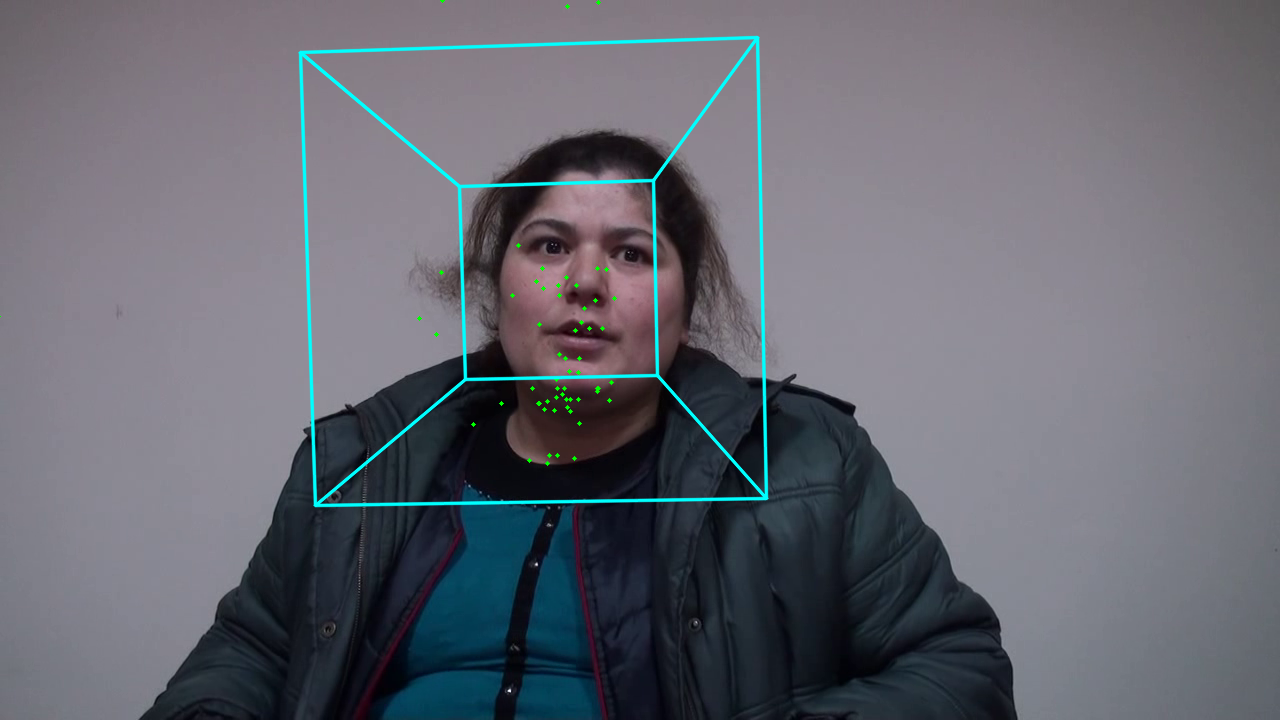
\includegraphics[width=\textwidth]{images/facial/recons_45_face_0_multiDDAE_egemaps.png} \\
    (e) reconstructed input at frame 45 from (10) in Table \ref{tab:multimodal_res}
    \end{minipage}
    \begin{minipage}[c]{0.42\linewidth}
    \centering
    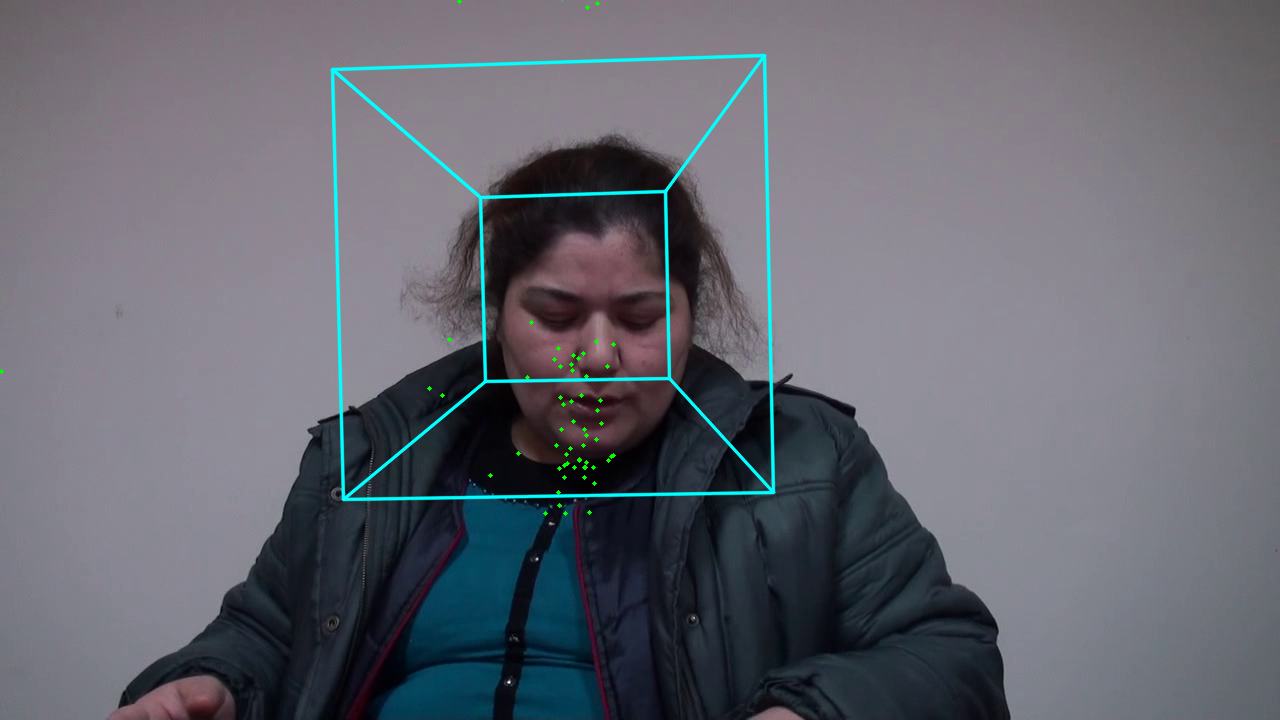
\includegraphics[width=\textwidth]{images/facial/recons_285_face_0_multiDDAE_egemaps.png} \\
    (f) reconstructed input at frame 285 from (10) in Table \ref{tab:multimodal_res}
    \end{minipage}
    \caption{Reconstruction of facial landmarks and head pose in Multimodal DDAEs from noisy input}
    \label{fig:reconstruction_multiDDAE}
\end{figure}


T-distributed Stochastic Neighbour Embedding (t-SNE) was proposed for dimensionality reduction and visualization of high-dimensional data in two or three dimensions \cite{maaten2008}. These following visualizations are generated using the Embedding Projector (\url{https://projector.tensorflow.org/}) with approximately 1000 iterations and 0.01 learning rate.

Before measuring the classification performance, Fisher Vectors (FVs) after feature selection are visualized via t-SNE as Figure \ref{fig:tsne_DDAEs}, which only concentrates on the best-performing bi-DDAEs and multi-DDAEs in Table \ref{tab:bimodal_res} and \ref{tab:multimodal_res}. As shown in Figure \ref{fig:tsne_DDAEs}, three, four, and five clusters can be easily identified in (a), (c) and (d) respectively that validate the better performance of DDAE architectures except bi-DDAE on eGeMAPS, whose visualization fails to show clear clusters in (b). In addition, DDAEs using MFCC as acoustic features help to produce more discriminative FVs (seen in (a) and (c)), which corresponds to the better performance on (1) in both \ref{tab:bimodal_res} and \ref{tab:multimodal_res}. The best performance of (1) in Table \ref{tab:multimodal_res} is validated through the visualization of FVs.


\begin{figure}[htb]
    \centering
    \small
    \begin{minipage}[c]{0.4\linewidth}
    \centering
    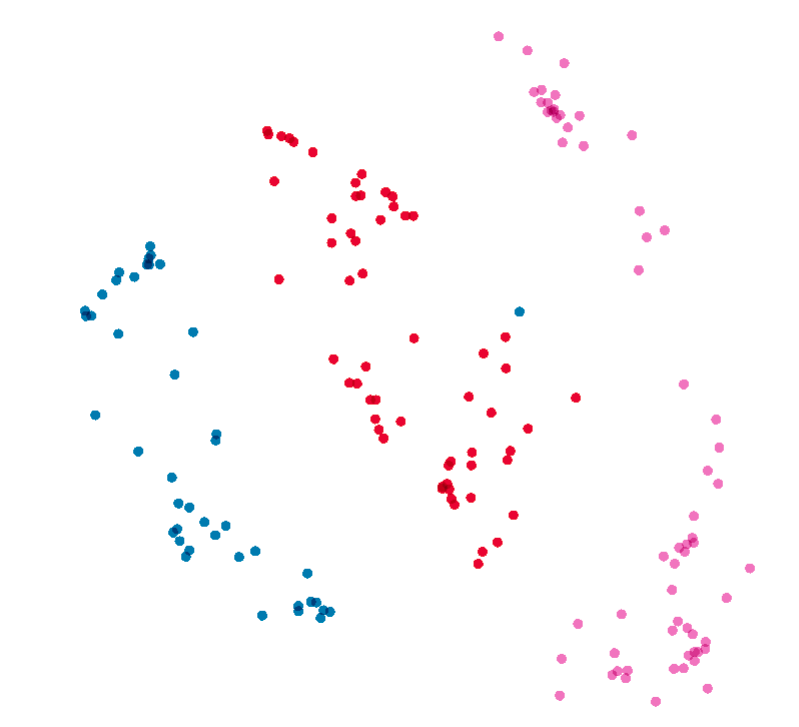
\includegraphics[height=4.8cm]{images/results/bi_DDAE_MFCC_tsne.png} \\
    (a) bi-DDAE (1) in Table \ref{tab:bimodal_res}
    \end{minipage}
    \begin{minipage}[c]{0.4\linewidth}
    \centering
    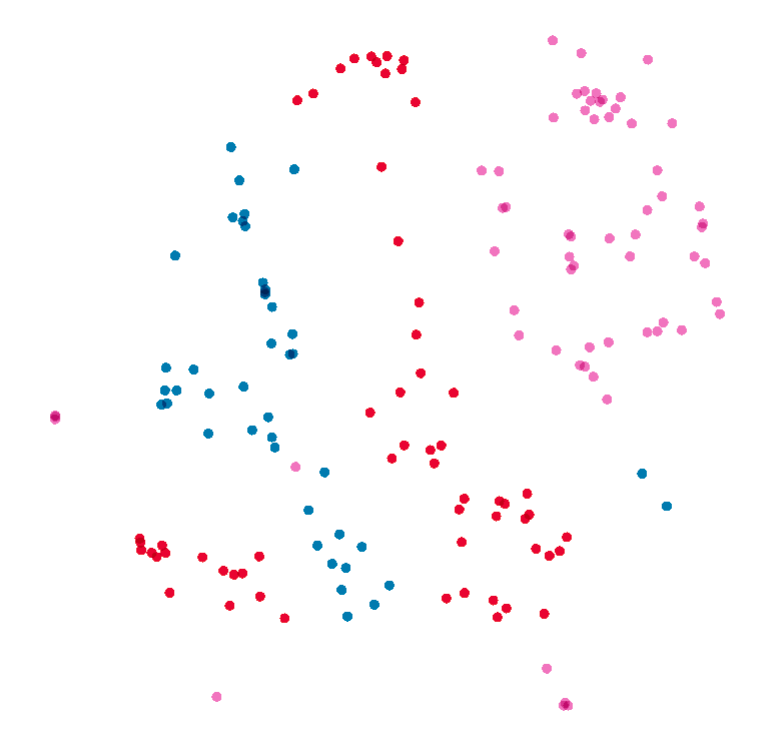
\includegraphics[height=4.8cm]{images/results/bi_DDAE_eGeMAPS_tsne.png} \\
    (b) bi-DDAE (10) in Table \ref{tab:bimodal_res}
    \end{minipage}
    \\
    \begin{minipage}[c]{0.4\linewidth}
    \centering
    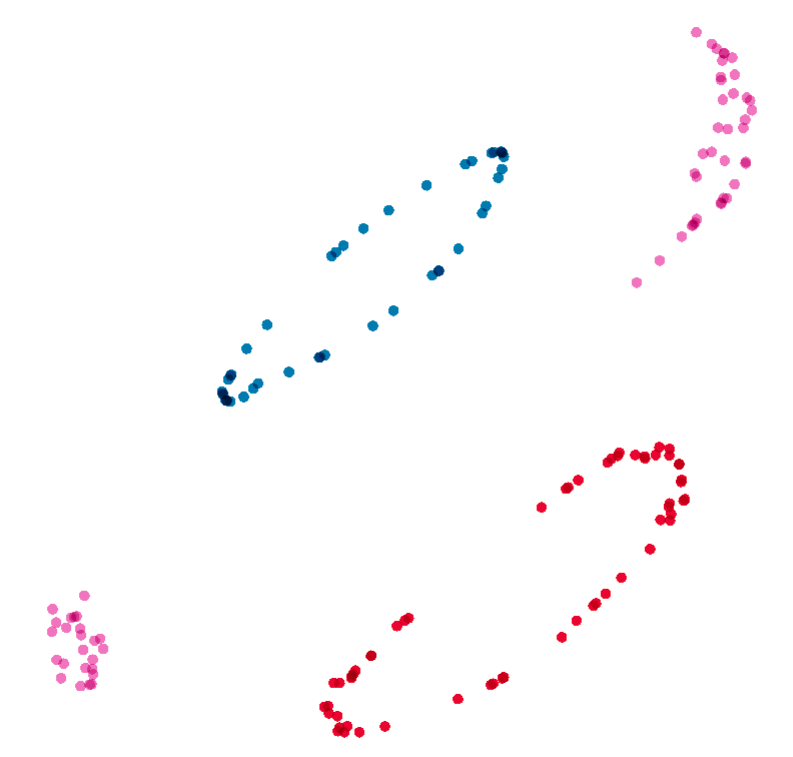
\includegraphics[height=4.8cm]{images/results/multi_DDAE_MFCC_tsne.png} \\
    (c) multi-DDAE (1) in Table \ref{tab:multimodal_res}
    \end{minipage}
    \begin{minipage}[c]{0.4\linewidth}
    \centering
    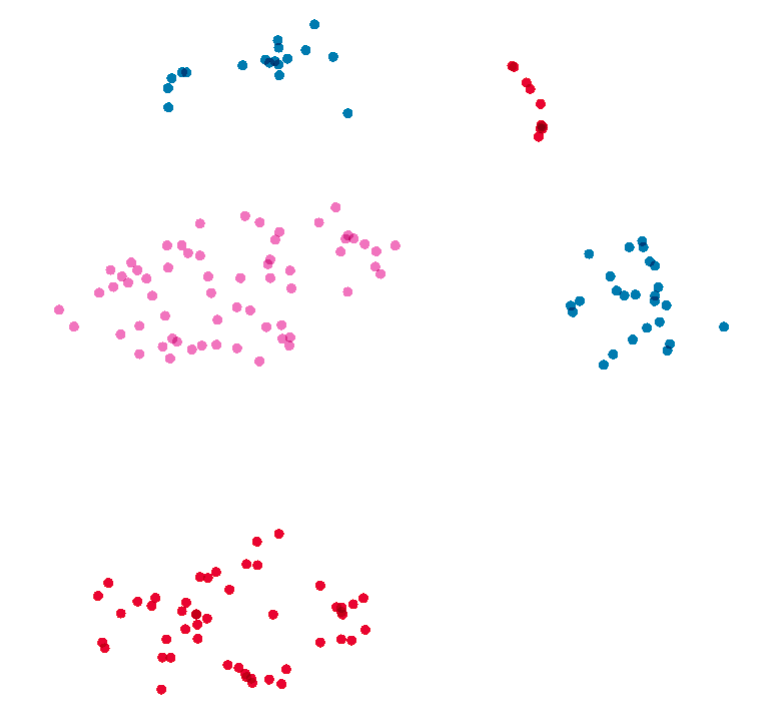
\includegraphics[height=5.1cm]{images/results/multi_DDAE_eGeMAPS_tsne.png} \\
    (d) multi-DDAE (10) in Table \ref{tab:multimodal_res}
    \end{minipage}
    \caption{Fisher vectors visualization in 2D space using t-SNE algorithm}
    \label{fig:tsne_DDAEs}
\end{figure}



\section{Textual Modality}

In the textual modality, the classification performance of different hyperparameter settings of document embeddings is represented first and the same Random Forest (RF) as the baseline are used for the classification. To evaluate the quality of document embeddings, I visualize the embedding space and list the word similarities and the document similarities, which are inferred by the embedding models. 

\subsection{Assessment of document embeddings}

Table \ref{tab:doc2vec_res} presents the experimental results for the document embedding models on the transcripts of interview sessions, and only the best-performing hyperparameter setting in both doc2vec models is listed. The full comparison of doc2vec models with different hyperparameter settings refers to Table \ref{tab:doc2vec_results} in Appendix and it is also visualized in a barchart as Figure \ref{fig:doc2vec_bar}.  


\begin{figure}[ht]
    \centering
    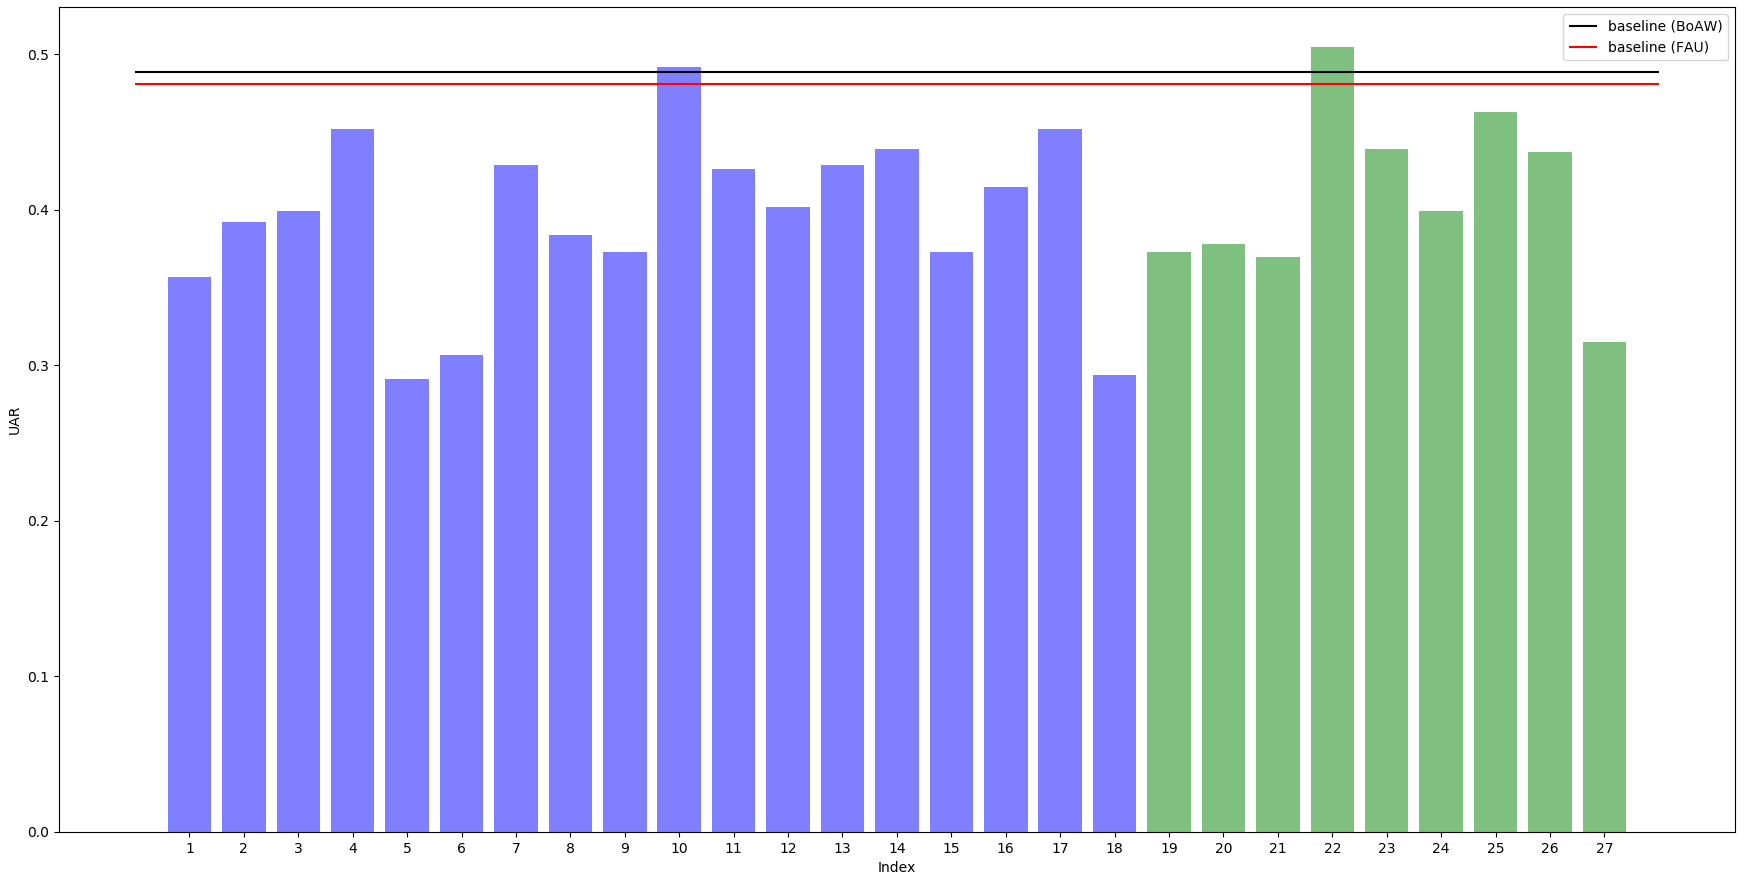
\includegraphics[width=\textwidth]{images/results/doc2vec.png}
    \caption{Barchart for the experimental results of doc2vec models indexed as Table \ref{tab:doc2vec_results}}
    \label{fig:doc2vec_bar}
\end{figure}

As illustrated in Table \ref{tab:doc2vec_res}, both PV-DM and PV-DBOW models achieve slightly better performance than the baseline. As their performance on sentiment analysis task \cite{lau2016}, the experimental results in BD recognition task show better performance in PV-DBOW in comparison with PV-DM (0.013 higher in UAR and 0.038 in F1 score). 
Additionally, I find that PV-DBOW models generally outperform PV-DM models in the hyperparameter settings as shown in Figure \ref{fig:doc2vec} and only the selected PV-DBOW and PV-DM models outperform the baseline while others do not.


\begin{table}[htb]
    \centering
    \small
    \caption{Comparison of proposed document embeddings on the transcripts (selected experimental results) with baseline results attached}
    \begin{tabular}{l|l|p{1.2cm}|p{1.5cm}|p{1.6cm}|l|l|l}
    \Xhline{2\arrayrulewidth}
        Index & Model & Vector size & Window size & Negative words & UAR & UAP & F1 \\
        \hline
        (10) & PV-DM & 50 & 10 & 5 & 0.492 & 0.481 & 0.486 \\
        \hline
        (22) & PV-DBOW & 50 & - & 5 & 0.505 & 0.544 & 0.524 \\
        \hline
        & \multicolumn{4}{l|}{Baseline (BoAW)} & 0.489 & 0.439 & 0.463 \\
        & \multicolumn{4}{l|}{Baseline (FAU)} & 0.481 & 0.528 & 0.503 \\
    \Xhline{2\arrayrulewidth}
    \end{tabular}
    \label{tab:doc2vec_res}
\end{table}



\subsection{Visualization and Qualitative Analysis}

The cosine similarity between similar words is first examined as Table \ref{tab:word_similarity}, in which top five similar words inferred by doc2vec models ((10) and (22) in Table \ref{tab:doc2vec_res}) with the target word 'good' are listed along with the translation. The similarity $|x - y|$ and distance $\langle x,y \rangle$ between two words are defined as $|x-y|^2 = |x|^2 + |y|^2 - 2\langle x,y\rangle$. Therefore, in the embedding space of doc2vec models, similar words should have high cosine similarity and a short distance between each other. 

As seen in Table \ref{tab:word_similarity}, the PV-DM model indeed shows a more meaningful embedding results as 'high', 'good' and 'important' are generally considered to be positively related with 'good' while 'least' and 'little' are considered to be negatively related. This indicates that words with similar meanings are mapped to similar positions in the embedding space \cite{mikolov2014}. On the other hand, the similar words inferred by PV-DBOW are not related to the word 'good' as the PV-DBOW model does not train the word vectors and these vectors remain randomly initialized values.


\begin{table}[htb]
    \centering
    \small
    \caption{Word similarities inferred by doc2vec models}
    \begin{tabular}{l|p{1cm}|p{1.5cm}|p{1.5cm}|p{1.5cm}|p{1.7cm}|p{1.5cm}}
        \Xhline{2\arrayrulewidth}
        \multicolumn{7}{l}{PV-DM} \\
        \Xhline{2\arrayrulewidth}
        word & \textbf{iyi} & azından & yüksek & iyisi & az & önemlisi \\
        \hline
        translation & \textbf{good} & least & high & good & little & important \\
        \hline
        similarity & - & 0.894 & 0.869 & 0.862 & 0.853 & 0.825 \\
        \Xhline{2\arrayrulewidth}
        \multicolumn{7}{l}{PV-DBOW} \\
        \Xhline{2\arrayrulewidth}
        word & \textbf{iyi} & yul bugavi & düşünü- lebir & ikamet- gahlarına & hastalıktır & içereni \\
        \hline
        translation & \textbf{good} & followings & it is considered of & to residence & disease & including \\
        \hline
        similarity & - & 0.613 & 0.607 & 0.603 & 0.599 & 0.589 \\
        \Xhline{2\arrayrulewidth}
    \end{tabular}
    \label{tab:word_similarity}
\end{table}


To extend the similarity from word-level to document-level, I randomly select one transcript of the interview session and use doc2vec models to inferred the similar documents, which should be also mapped to similar position in the embedding space \cite{mikolov2014}. Table \ref{tab:doc_sim_dm} presents the most similar and the least similar transcripts inferred by PV-DM to the target and Table \ref{tab:doc_sim_dbow} presents the same information but inferred by PV-DBOW. These two tables are attached at the end of this chapter. Since the mental state information exists in textual modality, the most similar transcript and the target in Table \ref{tab:doc_sim_dm} show a similar sentiment or emotion of the interviewee that he/she could be upset, helpless, or worried. The least similar transcript, however, shows nothing related to the target. Based on the same target, Table \ref{tab:doc_sim_dbow} shows that PV-DBOW maps transcripts to an embedding space in which similar transcripts share similar feelings of the subject.


\begin{figure}[htb]
    \centering
    \small
    \begin{minipage}{0.42\linewidth}
    \centering
    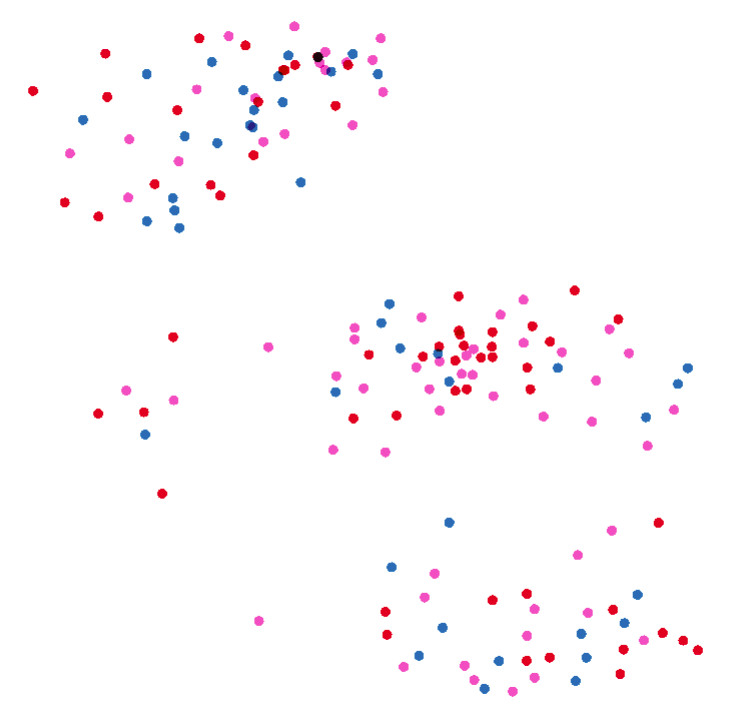
\includegraphics[width=6cm]{images/results/dm_tsne_2d.png} \\
    (a) PV-DM ((10) in Table \ref{tab:doc2vec_res})
    \end{minipage}
    \hfill
    \begin{minipage}{0.42\linewidth}
    \centering
    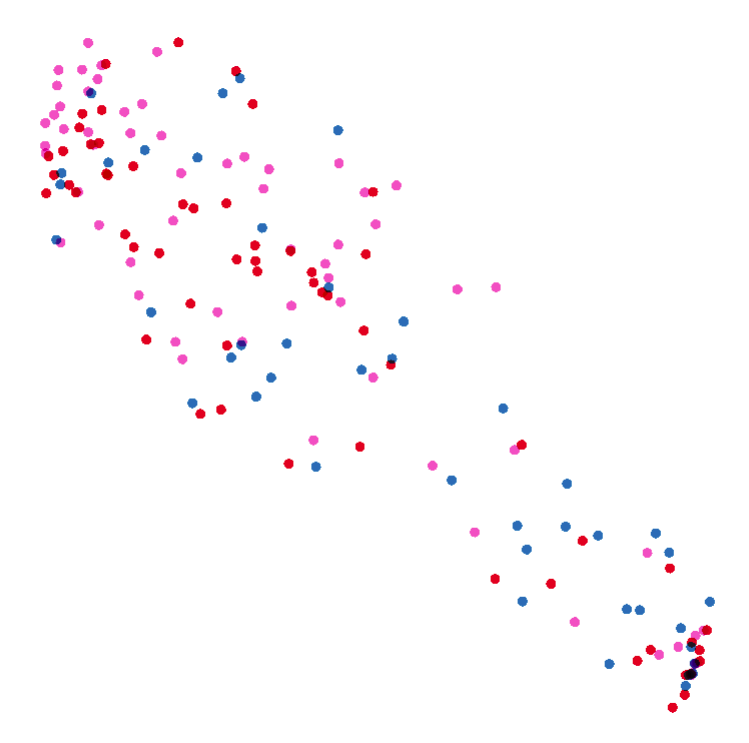
\includegraphics[width=6cm]{images/results/dbow_tsne_2d.png} \\
    (b) PV-DBOW ((22) in Table \ref{tab:doc2vec_res})
    \end{minipage}
    \caption{Document embeddings visualization in 2D space using t-SNE algorithm}
    \label{fig:doc2vec_vis_tsne}
\end{figure}


Similar as the visualization of Fisher Vectors (FVs), Figure \ref{fig:doc2vec_vis_tsne} displays the t-SNE visualization in 2-dimensional space for doc2vec models. The visualization is completed using the Embedding Projector (\url{https://projector.tensorflow.org/}) with around 1000 iteration and 0.01 learning rate. The colours in Figure \ref{fig:doc2vec_vis_tsne} indicate the same classes, of which the data points should be close to one another. Four clusters can be observed in (a) of Figure \ref{fig:doc2vec_vis_tsne} and two clusters in (b). There are, however, data points of more than one class in each cluster that impair the separation between different classes. This could account for the performance of doc2vec models on the classification of BD symptoms.


\section{Multimodal Feature Fusion}

With bi-DDAEs and multi-DDAEs on audio-visual modality and doc2vec models on textual modality, a total of 8 combinations are presented as Table \ref{tab:fusion_res}, in which the bi-DDAEs, multi-DDAEs and doc2vec models are the best-performing ones corresponding to Table \ref{tab:bimodal_res}, Table \ref{tab:multimodal_res} and Table \ref{tab:doc2vec_res} respectively.

\begin{table}[htb]
    \centering
    \small
    \caption{Comparison of proposed framework with feature fusion on audio-visual modality and textual modality. The best performance is in \textbf{bold} for each metric.}
    \begin{tabular}{l|l|l|l|l|l}
    \Xhline{2\arrayrulewidth}
        Index & Audio-Visual modality & Textual modality & UAR & UAP & F1  \\
        \hline
        (1) & bi-DDAE (MFCC) & PV-DM & 0.659 & 0.683 & 0.671 \\
        (2) & bi-DDAE (MFCC) & PV-DBOW & 0.593 & 0.602 & 0.597 \\
        (3) & bi-DDAE (eGeMAPS) & PV-DM & 0.571 & 0.624 & 0.596 \\
        (4) & bi-DDAE (eGeMAPS) & PV-DBOW & 0.603 & 0.633 & 0.618 \\
        (5) & multi-DDAE (MFCC) & PV-DM & \textbf{0.709} & \textbf{0.734} & \textbf{0.721} \\
        (6) & multi-DDAE (MFCC) & PV-DBOW & 0.667 & 0.680 & 0.673 \\
        (7) & multi-DDAE (eGeMAPS) & PV-DM & 0.675 & 0.708 & 0.691 \\
        (8) & multi-DDAE (eGeMAPS) & PV-DBOW & 0.659 & 0.671 & 0.665 \\
    \Xhline{2\arrayrulewidth}
    \end{tabular}
    \label{tab:fusion_res}
\end{table}

The early fusion strategy is applied to concatenate the compact-size vectors from audio-visual modality and textual modality to obtain a joint feature for the Multi-Task Neural Network (MTNN). The dimension of fused features is 150, the sum of 100-dimensional audio-visual features after feature selection and 50-dimensional document embeddings. The MTNN is then fine-tuned on the pre-determined development set with overfitting addressed. As Table \ref{tab:fusion_res} shows, the best performing framework is based on the fusion of (1) multi-DDAE using MFCC as acoustic features and (10) PV-DM document embeddings and the UAR reaches up to 0.709 and F1 score to 0.721. 

While PV-DBOW alone performs better than PV-DM, PV-DM fused with DDAEs shows a higher UAR and F1 score than PV-DBOW fused with DDAEs, indicating complementary mental information appended to the fused feature.



\subsection{Comparison with Competing Frameworks}

Since the experiments are based on the pre-determined partition of the BD corpus, the proposed framework can be directly compared with the frameworks proposed in AVEC2018 \cite{ringeval2018}. Table \ref{tab:avec2018_compare} lists the experimental results produced by different frameworks on the development set. It is clear that my framework outperforms the frameworks proposed by \cite{du2018} and \cite{syed2018} in both UAR and accuracy. Furthermore, my framework achieves the same accuracy as \cite{yang2018} with a very close UAR (only 0.005 lower). Therefore, the proposed framework, which is based on a multi-DDAE to encode audio-visual modality and a PV-DM to embed textual modality, achieves the state-of-the-art performance on BD recognition.

\begin{table}[h]
    \small
    \centering
    \caption{Comparison of the proposed framework (which performance is in \textbf{bold}) with the competing frameworks in AVEC2018}
    \begin{tabular}{l|l|l}
    \Xhline{2\arrayrulewidth}
        Framework & UAR (dev) & Accuracy (dev) \\
        \hline
        Yang \textit{et al.} 2018 & 0.714 & 0.717 \\
        \hline
        Du \textit{et al.} 2018 & 0.651 & 0.650 \\
        \hline
        Xing \textit{et al.} 2018 & 0.868 & NA \\
        \hline
        Syed \textit{et al.} 2018 & 0.635 & NA \\
        \hline
        \textbf{This work} 2019 & \textbf{0.709} & \textbf{0.717} \\
    \Xhline{2\arrayrulewidth}
    \end{tabular}
    \label{tab:avec2018_compare}
\end{table}


\subsection{Generalization}

To validate the generalization of the proposed framework, a 10-fold cross-validation is implemented for 8 frameworks listed in Table \ref{tab:fusion_res}. As there are $104 + 60 = 164$ samples in the corpus, 16 samples are selected as the test set with the rest as the training set. In Figure \ref{fig:errorbar}, the index of frameworks corresponds to Table \ref{tab:fusion_res}, in which (5) performs the best on pre-determined development set. 

Figure \ref{fig:errorbar} displays the means, visualized as bars, and the variances, visualized as error bars, which are calculated from the UAR on 10-fold cross-validation of different fusion frameworks. It is worth noting that (5) fusion framework still has the highest averaged UAR at approximately 0.60 and it can reach up to 0.91 UAR in one train/test split. For the rest of fusion frameworks, the averaged UAR in (3) and (4) is slightly higher than 0.50 and the second best-performing one, (7) has only the average UAR over 0.54. Therefore, framework (3), (4) and (7) are demonstrated less effective than others, and more likely to suffer from overfitting to the train/test split defined in AVEC2018. 

\begin{figure}[htb]
    \centering
    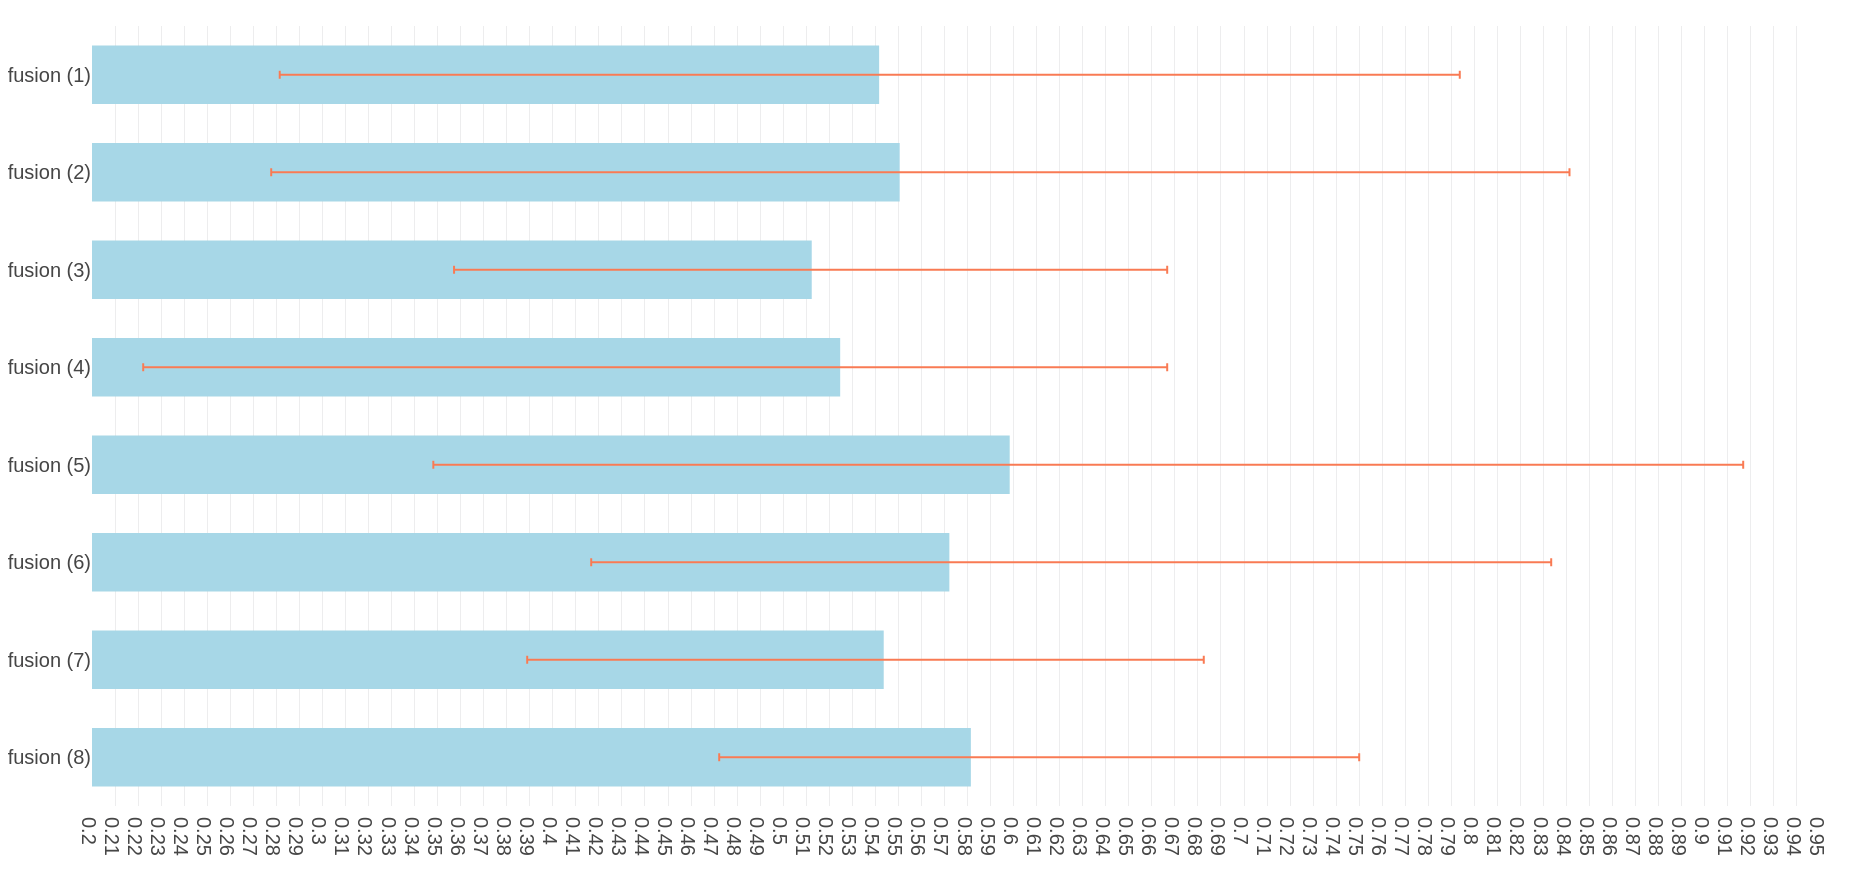
\includegraphics[width=\textwidth]{images/results/barchart_cv.png}
    \caption{Barchart of the averaged UAR and variance generated via a 10-fold cross-validation on different fusion frameworks}
    \label{fig:errorbar}
\end{figure}




\begin{table}[h]
    \centering
    \small
    \caption{Document similarities inferred by PV-DM model}
    \begin{tabular}{p{6.5cm}|p{6cm}}
        \Xhline{2\arrayrulewidth}
        \textless Target\textgreater ...görüştükten sonra bu tarafa geçirdiler Ben dediğimi burada ızdırap çeken bir insan var ya yanında bir portre var bunun kalemler falan var öyle Alev yanarken alevler çıkarkenki bir yanıt var bilmiyorum ama neden çok çaresiz çok çaresiz duruyor yani sanki yüzünü insanın yüzüne bakmaya yüzü kalmamış gibi kafasını falan aynı rahmetli babama da benzettim yanında çaresiz bir insan görüyorum burada çok çaresiz ne yapacağını bilmeyen kendine şaşırmış bir tek sandalyesi... & \textless Translation\textgreater ...There is a person who suffers from what I said here or there is a portrait of it. There is a pencil or something. I don't know why there is an answer while the flame is burning, but why is it so desperate and so desperate, it's as if you don't have a face to face. I've seen a helpless person next to my deceased father likened here too helpless does not know what to do self-surprised single chair... \\
        \hline
        \multicolumn{2}{l}{Similarity: 0.796} \\
        \hline
        \textless Most Similar\textgreater ...Bir hatırlatır misiniz Annemi babamı üzmem en büyük yanlış ve toplumla yargıda aradı davrandı için toplumu kafaya taktım saplantı yaptım mutlu ve aile tablosu bu sorunu daha önce de soruldu arkadaşa bir doğum günü şakası yapmıştı koydum en güzel hatıra... & \textless Translation\textgreater ...Could you remind me of my mother to upset my father the biggest wrong and looked for the society in the judiciary pretended I was obsessed with the society and the family table was happy before I was asked this problem a friend had made a birthday joke I said the most beautiful souvenir... \\
        \hline
        \multicolumn{2}{l}{Similarity: -0.031} \\
        \hline
        \textless Least Similar\textgreater ...Hepsi- burada evlendiniz mi Anlatır mısınız ya ne düşündüğünü ve istediğini üzere bir adamla ağlıyor gibi kötü teşekkür ederiz... & \textless Translation\textgreater ...Did you ever marry here? Can you tell me or thank you badly as if you are crying with a man as he thinks and wants?... \\
        \Xhline{2\arrayrulewidth}
    \end{tabular}
    \label{tab:doc_sim_dm}
\end{table}

\begin{table}[h]
    \centering
    \small
    \caption{Document similarities inferred by PV-DBOW model}
    \begin{tabular}{p{6.5cm}|p{6cm}}
        \Xhline{2\arrayrulewidth}
        \textless Target\textgreater ...görüştükten sonra bu tarafa geçirdiler Ben dediğimi burada ızdırap çeken bir insan var ya yanında bir portre var bunun kalemler falan var öyle Alev yanarken alevler çıkarkenki bir yanıt var bilmiyorum ama neden çok çaresiz çok çaresiz duruyor yani sanki yüzünü insanın yüzüne bakmaya yüzü kalmamış gibi kafasını falan aynı rahmetli babama da benzettim yanında çaresiz bir insan görüyorum burada çok çaresiz ne yapacağını bilmeyen kendine şaşırmış bir tek sandalyesi... & \textless Translation\textgreater ...There is a person who suffers from what I said here or there is a portrait of it. There is a pencil or something. I don't know why there is an answer while the flame is burning, but why is it so desperate and so desperate, it's as if you don't have a face to face. I've seen a helpless person next to my deceased father likened here too helpless does not know what to do self-surprised single chair... \\
        \hline
        \multicolumn{2}{l}{Similarity: 0.879} \\
        \hline
        \textless Most Similar\textgreater ...Pardon unuttum tablosu değil Mutsuz bir aile tablosu oda dolusu veri tablosu çocuklarıyla ve eşiyle mutlu arada güçlü bir sevgi bağı var doğru mu Buse Bu kadar yeter yaşamımızdaki en güzel hatırınız anlatır mısın vallahi öyle yaşamındaki en güzel hatıram alkollüydü arkadaşlarla kafamız sarhoşluk yani kafam iyi değil Çok sarhoştum güzel bir arkadaşlık arkaya vurulmuştu ama o espriyi Söyleyemem çok oturdum güzel bir espri yapmıştım da arkadaşlarımı Espriye görmüştü... & \textless Translation\textgreater ...Sorry I forgot the table is not an unhappy family table room full of data table Is there a strong bond of love between the children and his wife happy Buse Do you tell me the most beautiful memory in our life, I swear that the most beautiful memories of life in my life was drunk with friends I was very drunk a beautiful friendship was shot in the back, but I can not say that joke sat a nice joke I had seen my friends joke... \\
        \hline
        \multicolumn{2}{l}{Similarity: 0.171} \\
        \hline
        \textless Least Similar\textgreater ...Hepsi- burada evlendiniz mi Anlatır mısınız ya ne düşündüğünü ve istediğini üzere bir adamla ağlıyor gibi kötü teşekkür ederiz... & \textless Translation\textgreater ...Did you ever marry here? Can you tell me or thank you badly as if you are crying with a man as he thinks and wants?... \\
        \Xhline{2\arrayrulewidth}
    \end{tabular}
    \label{tab:doc_sim_dbow}
\end{table}


\chapter{Summary and Conclusion}
\label{ch:summary}


This work proposes an automatic framework for Bipolar Disorder (BD) recognition. As the BD corpus contains the clinical interviews with patients, all possible modalities in the interview recordings are utilized. 

For the audio-visual modality, Multimodal Deep Denoising Autoencoders (multi-DDAEs) are used to learn the joint representations, which are then encoded with the dynamics into Fisher Vectors (FVs). For the textual modality, document embeddings are inferred by Paragraph Vector (PV-DM) models that are based on the transcripts of interview videos. To reach the final decision, the early fusion strategy is applied to fuse features and for the classification task of mania levels, a Multi-Task Neural Network is implemented to address the overfitting issue with a joint loss on an addition regression task of YMRS score.

The multi-DDAEs take advantage of the shared representations from acoustic features, either MFCC or eGeMAPS, and visual features including facial landmarks, eye gaze, head pose and action units. On the other hand, the document embeddings produced by PV-DM provide complementary information on mental states and help to improve the classification performance in the final framework. The experimental results show that the proposed framework outperformed the baseline system and the frameworks \cite{du2018} and \cite{syed2018} in AVEC2018 with 0.709 in UAR and 0.717 in accuracy, and the cross-validation demonstrates its generalization across the BD corpus.

In the current framework, the multi-DDAEs focus the shared representation learning on all available modalities without considering the characteristics of each modality alone or the semantic interface between different modalities. Furthermore, the temporal information is simply captured by computing the dynamics of representations in contiguous frames. I plan to further the multi-DDAE architectures by introducing more layers (which could be Convolutional or Pooling layers) in the encoder part to capture the spatial information for some modalities, such as facial landmarks, and correlating and decoupling modalities via a sparse, semantics interface, like the convergence-divergence zone \cite{meyer2009}. Moreover, architectures like Recurrent Neural Networks (RNNs) are recommended to be investigated on encoding the shared representation within variable-length intervals. Finally, it would be worthwhile to experiment with the proposed framework on other but relevant mental state based challenges. AVEC2019 presents a challenge on human state-of-mind, which constantly shifts and is reflected by the emotions. I would like to apply this framework to this challenge and test its performance on other emotion-based recognition tasks.

\let\svaddcontentsline\addcontentsline
\renewcommand\addcontentsline[3]{%
  \ifthenelse{\equal{#1}{lof}}{}%
  {\ifthenelse{\equal{#1}{lot}}{}{\svaddcontentsline{#1}{#2}{#3}}}}

\appendix
\addcontentsline{toc}{chapter}{Appendix}
\chapter{Complete Experimental Results}
\label{ch:appendix}
\section{Deep Denoising Autoencoders}
\label{sec:DDAE_full}

In the following Table \ref{tab:unimodal_res_full}, \ref{tab:bimodal_res_full} and \ref{tab:multimodal_res_full}, the complete experimental results are provided for the Deep Denoising Autoencoders in the feature learning of the audio-visual modality. The evaluation metrics are Unweighted Average Recall (UAR), Unweighted Average Precision (UAP) and F1 score. The metrics in \textbf{bold} indicate the best-performing hyperparameter setting within one DDAE architectures. For instance, (4) in Table \ref{tab:unimodal_res_full} outperforms other architectures within the uni-DDAEs using facial landmarks ((1) to (12)).

\begin{table}[htb]
    \centering
    \small
    \caption{Complete list of the experimental results for the proposed Unimodal Deep Denoising Autoencoders. The best-performing results are in \textbf{bold} and the baseline results are attached at the end.}
    \begin{tabular}{l|l|p{1.25cm}|l|p{1.2cm}|l|l|l}
        \Xhline{2\arrayrulewidth}
        Index & Features & Hidden ratio & Noise & GMM kernel & UAR & UAP & F1 \\
        \hline
        (1) & Landmarks & 0.4 & 0.1 & 16 & 0.582 & 0.590 & 0.586 \\
        (2) & Landmarks & 0.4 & 0.1 & 32 & 0.563 & 0.575 & 0.569 \\
        (3) & Landmarks & 0.4 & 0.2 & 16 & 0.532 & 0.584 & 0.557 \\
        (4) & Landmarks & 0.4 & 0.2 & 32 & \textbf{0.624} & \textbf{0.692} & \textbf{0.656} \\
        (5) & Landmarks & 0.4 & 0.4 & 16 & 0.437 & 0.421 & 0.429 \\
        (6) & Landmarks & 0.4 & 0.4 & 32 & 0.614 & 0.622 & 0.618 \\
        (7) & Landmarks & 0.5 & 0.1 & 16 & 0.585 & 0.628 & 0.606 \\
        (8) & Landmarks & 0.5 & 0.1 & 32 & 0.579 & 0.577 & 0.578 \\
        (9) & Landmarks & 0.5 & 0.2 & 16 & 0.556 & 0.556 & 0.556 \\
        (10) & Landmarks & 0.5 & 0.2 & 32 & 0.606 & 0.635 & 0.620 \\
        (11) & Landmarks & 0.5 & 0.4 & 16 & 0.481 & 0.489 & 0.485 \\
        (12) & Landmarks & 0.5 & 0.4 & 32 & 0.611 & 0.620 & 0.615 \\
        \hline
        (13) & MFCC & 0.4 & 0.1 & 16 & 0.582 & 0.590 & 0.586 \\
        (14) & MFCC & 0.4 & 0.1 & 32 & \textbf{0.587} & \textbf{0.611} & \textbf{0.599} \\
        (15) & MFCC & 0.4 & 0.2 & 16 & 0.442 & 0.493 & 0.466 \\
        (16) & MFCC & 0.4 & 0.2 & 32 & 0.542 & 0.562 & 0.552 \\
        (17) & MFCC & 0.4 & 0.4 & 16 & 0.521 & 0.562 & 0.541 \\
        (18) & MFCC & 0.4 & 0.4 & 32 & 0.463 & 0.476 & 0.469 \\
        (19) & MFCC & 0.5 & 0.1 & 16 & 0.550 & 0.575 & 0.562 \\
        (20) & MFCC & 0.5 & 0.1 & 32 & 0.481 & 0.506 & 0.493 \\
        (21) & MFCC & 0.5 & 0.2 & 16 & 0.492 & 0.494 & 0.493 \\
        (22) & MFCC & 0.5 & 0.2 & 32 & 0.561 & 0.607 & 0.583 \\
        (23) & MFCC & 0.5 & 0.4 & 16 & 0.545 & 0.585 & 0.564 \\
        (24) & MFCC & 0.5 & 0.4 & 32 & 0.487 & 0.493 & 0.490 \\
        \hline
        (25) & eGeMAPS & 0.4 & 0.1 & 16 & 0.561 & 0.591 & 0.576 \\
        (26) & eGeMAPS & 0.4 & 0.1 & 32 & 0.426 & 0.423 & 0.424 \\
        (27) & eGeMAPS & 0.4 & 0.2 & 16 & 0.508 & 0.546 & 0.516  \\
        (28) & eGeMAPS & 0.4 & 0.2 & 32 & 0.524 & 0.532 & 0.528 \\
        (29) & eGeMAPS & 0.4 & 0.4 & 16 & 0.407 & 0.432 & 0.419 \\
        (30) & eGeMAPS & 0.4 & 0.4 & 32 & 0.511 & 0.563 & 0.536 \\
        (31) & eGeMAPS & 0.5 & 0.1 & 16 & 0.444 & 0.358 & 0.396 \\
        (32) & eGeMAPS & 0.5 & 0.1 & 32 & \textbf{0.632} & \textbf{0.654} & \textbf{0.637} \\
        (33) & eGeMAPS & 0.5 & 0.2 & 16 & 0.529 & 0.604 & 0.564 \\
        (34) & eGeMAPS & 0.5 & 0.2 & 32 & 0.590 & 0.619 & 0.604 \\
        (35) & eGeMAPS & 0.5 & 0.4 & 16 & 0.474 & 0.459 & 0.466 \\
        (36) & eGeMAPS & 0.5 & 0.4 & 32 & 0.563 & 0.585 & 0.574 \\
        \hline
        & \multicolumn{4}{l|}{Baseline (BoAW)} & 0.489 & 0.439 & 0.463 \\
        & \multicolumn{4}{l|}{Baseline (FAU)} & 0.481 & 0.528 & 0.503 \\
    \Xhline{2\arrayrulewidth}
    \end{tabular}
    \label{tab:unimodal_res_full}
\end{table}


\begin{table}[htb]
    \centering
    \small
    \caption{Complete list of the experimental results for the proposed Bimodal Deep Denoising Autoencoders. The best-performing results are in \textbf{bold}, and the baseline results and best results from Unimodal Deep Denoising Autoencoders are attached at the end.}
    \begin{tabular}{l|p{1.8cm}|p{1.25cm}|l|p{1.2cm}|l|l|l}
        \Xhline{2\arrayrulewidth}
        Index & Acoustic feature & Hidden ratio & Noise & GMM kernel & UAR & UAP & F1 \\
        \hline
        (1) & MFCC  & 0.4 & 0.1 & 16 & 0.492 & 0.455 & 0.473 \\
        (2) & MFCC  & 0.4 & 0.1 & 32 & \textbf{0.656} & \textbf{0.677} & \textbf{0.666} \\
        (3) & MFCC  & 0.4 & 0.2 & 16 & 0.632 & 0.644 & 0.638 \\
        (4) & MFCC  & 0.4 & 0.2 & 32 & 0.521 & 0.558 & 0.539 \\
        (5) & MFCC  & 0.4 & 0.4 & 16 & 0.413 & 0.490 & 0.448 \\
        (6) & MFCC  & 0.4 & 0.4 & 32 & 0.447 & 0.462 & 0.454 \\
        (7) & MFCC  & 0.5 & 0.1 & 16 & 0.487 & 0.472 & 0.479 \\
        (8) & MFCC  & 0.5 & 0.1 & 32 & 0.505 & 0.524 & 0.514 \\
        (9) & MFCC  & 0.5 & 0.2 & 16 & 0.471 & 0.522 & 0.495 \\
        (10) & MFCC  & 0.5 & 0.2 & 32 & 0.489 & 0.586 & 0.533 \\
        (11) & MFCC  & 0.5 & 0.4 & 16 & 0.444 & 0.449 & 0.446 \\
        (12) & MFCC  & 0.5 & 0.4 & 32 & 0.545 & 0.561 & 0.553 \\
        \hline
        (13) & eGeMAPS & 0.4 & 0.1 & 16 & 0.450 & 0.447 & 0.448 \\
        (14) & eGeMAPS & 0.4 & 0.1 & 32 & 0.566 & 0.569 & 0.567 \\
        (15) & eGeMAPS & 0.4 & 0.2 & 16 & 0.447 & 0.640 & 0.526 \\
        (16) & eGeMAPS & 0.4 & 0.2 & 32 & 0.516 & 0.600 & 0.555 \\
        (17) & eGeMAPS & 0.4 & 0.4 & 16 & 0.455 & 0.447 & 0.451 \\
        (18) & eGeMAPS & 0.4 & 0.4 & 32 & 0.511 & 0.538 & 0.524 \\
        (19) & eGeMAPS & 0.5 & 0.1 & 16 & \textbf{0.566} & \textbf{0.611} & \textbf{0.587} \\
        (20) & eGeMAPS & 0.5 & 0.1 & 32 & 0.495 & 0.506 & 0.500 \\
        (21) & eGeMAPS & 0.5 & 0.2 & 16 & 0.479 & 0.497 & 0.488 \\
        (22) & eGeMAPS & 0.5 & 0.2 & 32 & 0.458 & 0.459 & 0.458  \\
        (23) & eGeMAPS & 0.5 & 0.4 & 16 & 0.511 & 0.601 & 0.552 \\
        (24) & eGeMAPS & 0.5 & 0.4 & 32 & 0.519 & 0.607 & 0.560 \\
        \hline
        & \multicolumn{4}{l|}{Baseline (BoAW)} & 0.489 & 0.439 & 0.463 \\
        & \multicolumn{4}{l|}{Baseline (FAU)} & 0.481 & 0.528 & 0.503 \\
        \hline
        & \multicolumn{4}{l|}{Best Unimodal DDAE (Landmarks)} & 0.624 & 0.692 & 0.656 \\
        & \multicolumn{4}{l|}{Best Unimodal DDAE (MFCC)} & 0.587 & 0.611 & 0.599 \\
        & \multicolumn{4}{l|}{Best Unimodal DDAE (eGeMAPS)} & 0.632 & 0.654 & 0.637 \\
    \Xhline{2\arrayrulewidth}
    \end{tabular}
    \label{tab:bimodal_res_full}
\end{table}


\begin{table}[htb]
    \centering
    \small
    \caption{Complete list of the experimental results for the proposed Multimodal Deep Denoising Autoencoders. The best-performing results are in \textbf{bold}, and the baseline results and the best results from previous Deep Denoising Autoencoders are attached at the end.}
    \begin{tabular}{l|p{1.8cm}|p{1.25cm}|l|p{1.2cm}|l|l|l}
        \Xhline{2\arrayrulewidth}
        Index & Acoustic Feature & Hidden ratio & Noise & GMM kernel & UAR & UAP & F1 \\
        \hline
        (1) & MFCC  & 0.4 & 0.1 & 16 & 0.603 & 0.648 & 0.624 \\
        (2) & MFCC  & 0.4 & 0.1 & 32 & \textbf{0.656} & \textbf{0.678} & \textbf{0.667} \\
        (3) & MFCC  & 0.4 & 0.2 & 16 & 0.561 & 0.597 & 0.578  \\
        (4) & MFCC  & 0.4 & 0.2 & 32 & 0.566 & 0.573 & 0.569 \\
        (5) & MFCC  & 0.4 & 0.4 & 16 & 0.569 & 0.593 & 0.581 \\
        (6) & MFCC  & 0.4 & 0.4 & 32 & 0.459 & 0.475 & 0.467 \\
        (7) & MFCC  & 0.5 & 0.1 & 16 & 0.597 & 0.596 & 0.596 \\
        (8) & MFCC  & 0.5 & 0.1 & 32 & 0.582 & 0.605 & 0.593 \\
        (9) & MFCC  & 0.5 & 0.2 & 16 & 0.524 & 0.623 & 0.569 \\
        (10) & MFCC  & 0.5 & 0.2 & 32 & 0.569 & 0.578 & 0.573 \\
        (11) & MFCC  & 0.5 & 0.4 & 16 & 0.569 & 0.697 & 0.627 \\
        (12) & MFCC  & 0.5 & 0.4 & 32 & 0.529 & 0.528 & 0.528 \\
        \hline
        (13) & eGeMAPS & 0.4 & 0.1 & 16 & 0.603 & 0.717 & 0.655 \\
        (14) & eGeMAPS & 0.4 & 0.1 & 32 & 0.540 & 0.595 & 0.566 \\
        (15) & eGeMAPS & 0.4 & 0.2 & 16 & 0.495 & 0.504 & 0.499 \\
        (16) & eGeMAPS & 0.4 & 0.2 & 32 & 0.585 & 0.590 & 0.587 \\
        (17) & eGeMAPS & 0.4 & 0.4 & 16 & 0.489 & 0.514 & 0.501 \\
        (18) & eGeMAPS & 0.4 & 0.4 & 32 & 0.471 & 0.613 & 0.540 \\
        (19) & eGeMAPS & 0.5 & 0.1 & 16 & 0.442 & 0.462 & 0.452 \\
        (20) & eGeMAPS & 0.5 & 0.1 & 32 & \textbf{0.622} & \textbf{0.665} & \textbf{0.642} \\
        (21) & eGeMAPS & 0.5 & 0.2 & 16 & 0.574 & 0.570 & 0.572 \\
        (22) & eGeMAPS & 0.5 & 0.2 & 32 & 0.571 & 0.621 & 0.595 \\
        (23) & eGeMAPS & 0.5 & 0.4 & 16 & 0.484 & 0.536 & 0.507 \\
        (24) & eGeMAPS & 0.5 & 0.4 & 32 & 0.466 & 0.467 & 0.466 \\
        \hline
        & \multicolumn{4}{l|}{Baseline (BoAW)} & 0.489 & 0.439 & 0.463 \\
        & \multicolumn{4}{l|}{Baseline (FAU)} & 0.481 & 0.528 & 0.503 \\
        \hline
        & \multicolumn{4}{l|}{Best Unimodal DDAE (Landmarks)} & 0.624 & 0.692 & 0.656 \\
        & \multicolumn{4}{l|}{Best Unimodal DDAE (MFCC)} & 0.587 & 0.611 & 0.599 \\
        & \multicolumn{4}{l|}{Best Unimodal DDAE (eGeMAPS)} & 0.632 & 0.654 & 0.637 \\
        \hline
        & \multicolumn{4}{l|}{Best Bimodal DDAE (MFCC)} & 0.656 & 0.677 & 0.666 \\
        & \multicolumn{4}{l|}{Best Bimodal DDAE (eGeMAPS)} & 0.566 & 0.611 & 0.587 \\
    \Xhline{2\arrayrulewidth}
    \end{tabular}
    \label{tab:multimodal_res_full}
\end{table}


\section{Document Embedding}

This section includes the complete experimental results (Table \ref{tab:doc2vec_results}) for the document embedding models under different hyperparameter settings. The evaluation metrics are Unweighted Average Recall (UAR), Unweighted Average Precision (UAP) and F1 score. It is worthy noting that the window size is not defined in PV-DBOW architecture and the hierarchical softmax, as an alternative to softmax used in doc2vec models, is denoted as ``hs" in Table \ref{tab:doc2vec_results} ``Negative words" column. 

\begin{table}[ht]
    \small
    \centering
    \caption{Complete list of the experimental results for the proposed document embedding models. The best-performing results are in \textbf{bold} and the baseline results are attached at the end.}
    \begin{tabular}{l|l|p{1.2cm}|p{1.5cm}|p{1.6cm}|l|l|l}
         \Xhline{2\arrayrulewidth}
         Index & Model & Vector size & Window size & Negative words & UAR & UAP & F1 \\
         \hline
         (1) & PV-DM & 25 & 5 & 5 & 0.357 & 0.348 & 0.352 \\
         (2) & PV-DM & 25 & 5 & 10 & 0.392 & 0.406 & 0.394 \\
         (3) & PV-DM & 25 & 5 & hs & 0.399 & 0.402 & 0.400 \\
         (4) & PV-DM & 25 & 10 & 5 & 0.452 & 0.442 & 0.447 \\
         (5) & PV-DM & 25 & 10 & 10 & 0.291 & 0.290 & 0.279 \\
         (6) & PV-DM & 25 & 10 & hs & 0.307 & 0.295 & 0.290 \\
         (7) & PV-DM & 50 & 5 & 5 & 0.429 & 0.496 & 0.460 \\
         (8) & PV-DM & 50 & 5 & 10 & 0.384 & 0.405 & 0.394 \\
         (9) & PV-DM & 50 & 5 & hs & 0.373 & 0.376 & 0.374 \\
         (10) & PV-DM & 50 & 10 & 5 & \textbf{0.492} & \textbf{0.481} & \textbf{0.486} \\
         (11) & PV-DM & 50 & 10 & 10 & 0.426 & 0.455 & 0.440 \\
         (12) & PV-DM & 50 & 10 & hs & 0.402 & 0.598 & 0.480 \\
         (13) & PV-DM & 100 & 5 & 5 & 0.429 & 0.480 & 0.453 \\
         (14) & PV-DM & 100 & 5 & 10 & 0.439 & 0.513 & 0.473 \\
         (15) & PV-DM & 100 & 5 & hs & 0.373 & 0.379 & 0.375 \\
         (16) & PV-DM & 100 & 10 & 5 & 0.415 & 0.431 & 0.422\\
         (17) & PV-DM & 100 & 10 & 10 & 0.452 & 0.453 & 0.452 \\
         (18) & PV-DM & 100 & 10 & hs & 0.294 & 0.292 & 0.292 \\
         \hline
         (19) & PV-DBOW & 25 & - & 5 & 0.373 & 0.391 & 0.381 \\
         (20) & PV-DBOW & 25 & - & 10 & 0.378 & 0.397 & 0.387 \\
         (21) & PV-DBOW & 25 & - & hs & 0.370 & 0.383 & 0.376 \\
         (22) & PV-DBOW & 50 & - & 5 & \textbf{0.505} & \textbf{0.544} & \textbf{0.524} \\
         (23) & PV-DBOW & 50 & - & 10 & 0.439 & 0.461 & 0.450 \\
         (24) & PV-DBOW & 50 & - & hs & 0.399 & 0.435 & 0.416 \\
         (25) & PV-DBOW & 100 & - & 5 & 0.463 & 0.418 & 0.439 \\
         (26) & PV-DBOW & 100 & - & 10 & 0.437 & 0.454 & 0.445 \\
         (27) & PV-DBOW & 100 & - & hs & 0.315 & 0.330 & 0.315 \\
         \hline
         & \multicolumn{4}{l|}{Baseline (BoAW)} & 0.489 & 0.439 & 0.463 \\
         & \multicolumn{4}{l|}{Baseline (FAU)} & 0.481 & 0.528 & 0.503 \\
         \Xhline{2\arrayrulewidth}
    \end{tabular}
    \label{tab:doc2vec_results}
\end{table}
\singlespacing

\bibliographystyle{unsrt} 
\bibliography{reference} 

\end{document}
